\documentclass[twoside]{book}

% Packages required by doxygen
\usepackage{fixltx2e}
\usepackage{calc}
\usepackage{doxygen}
\usepackage[export]{adjustbox} % also loads graphicx
\usepackage{graphicx}
\usepackage[utf8]{inputenc}
\usepackage{makeidx}
\usepackage{multicol}
\usepackage{multirow}
\PassOptionsToPackage{warn}{textcomp}
\usepackage{textcomp}
\usepackage[nointegrals]{wasysym}
\usepackage[table]{xcolor}

% Font selection
\usepackage[T1]{fontenc}
\usepackage[scaled=.90]{helvet}
\usepackage{courier}
\usepackage{amssymb}
\usepackage{sectsty}
\renewcommand{\familydefault}{\sfdefault}
\allsectionsfont{%
  \fontseries{bc}\selectfont%
  \color{darkgray}%
}
\renewcommand{\DoxyLabelFont}{%
  \fontseries{bc}\selectfont%
  \color{darkgray}%
}
\newcommand{\+}{\discretionary{\mbox{\scriptsize$\hookleftarrow$}}{}{}}

% Page & text layout
\usepackage{geometry}
\geometry{%
  a4paper,%
  top=2.5cm,%
  bottom=2.5cm,%
  left=2.5cm,%
  right=2.5cm%
}
\tolerance=750
\hfuzz=15pt
\hbadness=750
\setlength{\emergencystretch}{15pt}
\setlength{\parindent}{0cm}
\setlength{\parskip}{3ex plus 2ex minus 2ex}
\makeatletter
\renewcommand{\paragraph}{%
  \@startsection{paragraph}{4}{0ex}{-1.0ex}{1.0ex}{%
    \normalfont\normalsize\bfseries\SS@parafont%
  }%
}
\renewcommand{\subparagraph}{%
  \@startsection{subparagraph}{5}{0ex}{-1.0ex}{1.0ex}{%
    \normalfont\normalsize\bfseries\SS@subparafont%
  }%
}
\makeatother

% Headers & footers
\usepackage{fancyhdr}
\pagestyle{fancyplain}
\fancyhead[LE]{\fancyplain{}{\bfseries\thepage}}
\fancyhead[CE]{\fancyplain{}{}}
\fancyhead[RE]{\fancyplain{}{\bfseries\leftmark}}
\fancyhead[LO]{\fancyplain{}{\bfseries\rightmark}}
\fancyhead[CO]{\fancyplain{}{}}
\fancyhead[RO]{\fancyplain{}{\bfseries\thepage}}
\fancyfoot[LE]{\fancyplain{}{}}
\fancyfoot[CE]{\fancyplain{}{}}
\fancyfoot[RE]{\fancyplain{}{\bfseries\scriptsize Generated by Doxygen }}
\fancyfoot[LO]{\fancyplain{}{\bfseries\scriptsize Generated by Doxygen }}
\fancyfoot[CO]{\fancyplain{}{}}
\fancyfoot[RO]{\fancyplain{}{}}
\renewcommand{\footrulewidth}{0.4pt}
\renewcommand{\chaptermark}[1]{%
  \markboth{#1}{}%
}
\renewcommand{\sectionmark}[1]{%
  \markright{\thesection\ #1}%
}

% Indices & bibliography
\usepackage{natbib}
\usepackage[titles]{tocloft}
\setcounter{tocdepth}{3}
\setcounter{secnumdepth}{5}
\makeindex

% Packages requested by user
\usepackage{mathdesign}

% Hyperlinks (required, but should be loaded last)
\usepackage{ifpdf}
\ifpdf
  \usepackage[pdftex,pagebackref=true]{hyperref}
\else
  \usepackage[ps2pdf,pagebackref=true]{hyperref}
\fi
\hypersetup{%
  colorlinks=true,%
  linkcolor=blue,%
  citecolor=blue,%
  unicode%
}

% Custom commands
\newcommand{\clearemptydoublepage}{%
  \newpage{\pagestyle{empty}\cleardoublepage}%
}

\usepackage{caption}
\captionsetup{labelsep=space,justification=centering,font={bf},singlelinecheck=off,skip=4pt,position=top}

%===== C O N T E N T S =====

\begin{document}

% Titlepage & ToC
\hypersetup{pageanchor=false,
             bookmarksnumbered=true,
             pdfencoding=unicode
            }
\pagenumbering{alph}
\begin{titlepage}
\vspace*{7cm}
\begin{center}%
{\Large A\+F\+E\+Pack for Electromagnetic }\\
\vspace*{1cm}
{\large Generated by Doxygen 1.8.14}\\
\end{center}
\end{titlepage}
\clearemptydoublepage
\pagenumbering{roman}
\tableofcontents
\clearemptydoublepage
\pagenumbering{arabic}
\hypersetup{pageanchor=true}

%--- Begin generated contents ---
\chapter{Notes on A\+F\+E\+Pack for Electromagnetic}
\label{index}\hypertarget{index}{}In fact, I make it not only for Electromagnetic calculation, but also for the general P\+DE cases.

In this note, the variational principles for electromagnetic is mainly based on Jian-\/\+Ming Jin\textquotesingle{}s the book “\+The Finite Element Method in Electromagnetics”.\hypertarget{index_nodeFEM}{}\section{Node Finite Elements}\label{index_nodeFEM}
Consider the P\+ED in a Lipschitz domain $ \Omega\in\mathcal{R}^d$, $ d=2,3$ \[ -\nabla \cdot (c(x)\nabla u) +a(x)u =f \qquad \in \Omega \] with right hand side $ f \in L^2(\Omega)^d $.

The boundary condition is the homogeneous Dirichlet boundary condition \[ u = b \qquad on \ \partial\Omega_1 \] and the homogeneous Neumann boundary condition \[ \hat{n}\cdot c(x)\nabla u + q(x)u = g \qquad on \ \partial\Omega_2 \] provided that a,c,q is real or complex and $ \hat{n}$is the outward normal from S, where $ \partial\Omega_1+\partial\Omega_2 = \partial\Omega $\hypertarget{index_forms}{}\subsection{Vartiational Formulation}\label{index_forms}
by applying the first scalar Green\textquotesingle{}s theorem \[ \int_\Omega v \nabla \cdot (c\nabla u) + c(\nabla v) \cdot (\nabla u) dV = \oint_{\partial\Omega} cv\frac{\partial u}{\partial n}dS \] ~\newline
and the boundary conditions above, we can get \[ \int_\Omega c(\nabla v) \cdot (\nabla u)dV +\int_\Omega a(x)uv dV = \int_\Omega fv dV + \oint_{\partial\Omega_2} v(g-q(x)u)dS \] the forms \[ a(u,v) := \int_\Omega c(\nabla v) \cdot (\nabla u) dV +\int_\Omega a(x)uv dV+\oint_{\partial\Omega_2}q(x)vudS \] \[ rhs(v) := \int_\Omega fv dV + \oint_{\partial\Omega_2} vgdS \]\hypertarget{index_exp1}{}\subsection{Example1}\label{index_exp1}
The computational domain is $[-1,1]\times [-1,1]$. The parameters \[ c(x) = 1 ,\quad a(x) = 0 \quad and \quad f = 2\pi^2\sin(\pi x)\sin(\pi y) \] the boundary parameters \[ b = 0, q(x) = 0 ,\quad and \quad g = \left\{ \begin{array}{ll} \pi \sin(\pi x) &\quad x \in [-1,1] \quad and \quad y=-1 \\ -\pi \sin(\pi y) &\quad x = 1 \quad and \quad y \in [-1,1] \\ -\pi \sin(\pi x) &\quad x \in [-1,1] \quad and \quad y=1 \\ \pi \sin(\pi y) &\quad x = -1 \quad and \quad y \in [-1,1] \end{array}\right. \] The exact solution is \[ u=\sin(\pi x)\sin(\pi y)\]

\href{../../example1.tiff}{\tt This figure} shows the results of Example.\hypertarget{index_vectorFEM}{}\section{Vector Finite Elements}\label{index_vectorFEM}
consider the vector-\/valued model problem \[ \nabla \times (c(x) \nabla \times \mathbf{u}) +a(x) \mathbf{u} = \mathbf{f} \qquad \in \Omega \] The boundary conditions are the homogenous Dirichlet boundary condition \[ \hat{n} \times \mathbf{u} = b \qquad on \ \partial\Omega_1 \] and the homogeneous Neumann boundary condition \[ c(x)\hat{n}\times (\nabla \times \mathbf{u}) + q(x)\hat{n}\times (\hat{n}\times \mathbf{u}) = \mathbf{g} \qquad on \ \partial\Omega_2 \] with $\partial\Omega_1+\partial\Omega_2=\partial\Omega$, a,c,and b,q are real(complex) numbers or functions.\hypertarget{index_forms}{}\subsection{Vartiational Formulation}\label{index_forms}
Invoking the first vector Green\textquotesingle{}s theorem and vector identity \[ \int_\Omega (c\nabla \times \mathbf{v}) \cdot (\nabla \times \mathbf{u}) - \mathbf{v} \cdot (\nabla \times (c\nabla \times \mathbf{u})) dV = \oint_{\partial \Omega} c(\mathbf{v}\times \nabla \times \mathbf{u}) \cdot \hat{n} dS \] \[ (\mathbf{v}\times \nabla \times\mathbf{u}) \cdot \hat{n} = (\hat{n}\times \mathbf{v}) \cdot (\nabla \times \mathbf{u})=-\mathbf{v}\cdot (\hat{n} \times (\nabla \times \mathbf{u})) \] applying the boundary conditions we obtain \[ \int_\Omega c(\nabla \times \mathbf{v})\cdot(\nabla\times \mathbf{u})dV+\int_\Omega a(x)\mathbf{u}\cdot\mathbf{v} dV= \int_\Omega \mathbf{f}\cdot\mathbf{v}dV-\oint_{\partial \Omega}\mathbf{v}\cdot(\mathbf{g}-q(x)\hat{n}\times(\hat{n}\times\mathbf{u}))dS \] the forms \[ a(\mathbf{u},\mathbf{v}) := \int_\Omega c(\nabla \times \mathbf{v})\cdot(\nabla\times \mathbf{u})dV+\int_\Omega a(x)\mathbf{u}\cdot\mathbf{v} dV+\oint_{\partial\Omega_2}q(x)(\hat{n}\times\mathbf{u})\cdot(\hat{n}\times\mathbf{v})dS \] \[ rhs(\mathbf{v}) := \int_\Omega \mathbf{f}\cdot\mathbf{v}dV-\oint_{\partial \Omega}\mathbf{v}\cdot \mathbf{g}dS \]\hypertarget{index_exp}{}\subsection{Example}\label{index_exp}
The computational domain is $[-1,1]\times [-1,1]$. The parameters \[ c(x) = 1 ,\quad a(x) = 1 \quad and \quad f = \left( \begin{array}{l} (2\pi^2+1)\cos(\pi x)\sin(\pi y)\\ -(2\pi^2+1)\sin(\pi x)\cos(\pi y) \end{array}\right) \] the boundary parameters \[ b = 0, q(x) = 0 ,\quad and \quad g = \left\{ \begin{array}{ll} (-2\pi \cos(\pi x),0) &\quad x \in [-1,1] \quad and \quad y=-1 \\ (0,-2\pi \cos(\pi y)) &\quad x = 1 \quad and \quad y \in [-1,1] \\ (2\pi \cos(\pi x),0) &\quad x \in [-1,1] \quad and \quad y=1 \\ (0,2\pi \cos(\pi y)) &\quad x = -1 \quad and \quad y \in [-1,1] \end{array}\right. \] The exact solution is \[ u=\left( \begin{array}{l} \cos(\pi x)\sin(\pi y)\\ -\sin(\pi x)\cos(\pi y) \end{array}\right) \]

\href{../../example2.tiff}{\tt This figure} shows the results of Example 
\chapter{Hierarchical Index}
\section{Class Hierarchy}
This inheritance list is sorted roughly, but not completely, alphabetically\+:\begin{DoxyCompactList}
\item \contentsline{section}{Geometry\+Cache$<$ D\+IM $>$}{\pageref{struct_geometry_cache}}{}
\begin{DoxyCompactList}
\item \contentsline{section}{Edge\+Cache$<$ value\+\_\+type, D\+IM $>$}{\pageref{struct_edge_cache}}{}
\item \contentsline{section}{Edge\+Cache$<$ value\+\_\+type, D\+IM $>$}{\pageref{struct_edge_cache}}{}
\item \contentsline{section}{Element\+Cache$<$ value\+\_\+type, D\+IM $>$}{\pageref{struct_element_cache}}{}
\item \contentsline{section}{Element\+Cache$<$ value\+\_\+type, D\+IM $>$}{\pageref{struct_element_cache}}{}
\end{DoxyCompactList}
\item \contentsline{section}{Solution\+Cache$<$ value\+\_\+type $>$}{\pageref{struct_solution_cache}}{}
\item \contentsline{section}{ui\+Experiment}{\pageref{classui_experiment}}{}
\end{DoxyCompactList}

\chapter{Class Index}
\section{Class List}
Here are the classes, structs, unions and interfaces with brief descriptions\+:\begin{DoxyCompactList}
\item\contentsline{section}{\mbox{\hyperlink{struct_edge_cache}{Edge\+Cache$<$ value\+\_\+type, D\+I\+M $>$}} }{\pageref{struct_edge_cache}}{}
\item\contentsline{section}{\mbox{\hyperlink{struct_element_cache}{Element\+Cache$<$ value\+\_\+type, D\+I\+M $>$}} }{\pageref{struct_element_cache}}{}
\item\contentsline{section}{\mbox{\hyperlink{struct_geometry_cache}{Geometry\+Cache$<$ D\+I\+M $>$}} }{\pageref{struct_geometry_cache}}{}
\item\contentsline{section}{\mbox{\hyperlink{struct_solution_cache}{Solution\+Cache$<$ value\+\_\+type $>$}} }{\pageref{struct_solution_cache}}{}
\item\contentsline{section}{\mbox{\hyperlink{classui_experiment}{ui\+Experiment}} }{\pageref{classui_experiment}}{}
\end{DoxyCompactList}

\chapter{File Index}
\section{File List}
Here is a list of all files with brief descriptions\+:\begin{DoxyCompactList}
\item\contentsline{section}{\mbox{\hyperlink{mainpage_8h}{mainpage.\+h}} }{\pageref{mainpage_8h}}{}
\item\contentsline{section}{complex\+\_\+edge\+\_\+\+T\+H\+F\+E\+M/\mbox{\hyperlink{complex__edge___t_h_f_e_m_2_d_8d}{D.\+d}} }{\pageref{complex__edge___t_h_f_e_m_2_d_8d}}{}
\item\contentsline{section}{complex\+\_\+edge\+\_\+\+T\+H\+F\+E\+M/\mbox{\hyperlink{complex__edge___t_h_f_e_m_2datacache_8cpp}{datacache.\+cpp}} }{\pageref{complex__edge___t_h_f_e_m_2datacache_8cpp}}{}
\item\contentsline{section}{complex\+\_\+edge\+\_\+\+T\+H\+F\+E\+M/\mbox{\hyperlink{complex__edge___t_h_f_e_m_2datacache_8h}{datacache.\+h}} }{\pageref{complex__edge___t_h_f_e_m_2datacache_8h}}{}
\item\contentsline{section}{complex\+\_\+edge\+\_\+\+T\+H\+F\+E\+M/\mbox{\hyperlink{complex__edge___t_h_f_e_m_2emdefs_8h}{emdefs.\+h}} }{\pageref{complex__edge___t_h_f_e_m_2emdefs_8h}}{}
\item\contentsline{section}{complex\+\_\+edge\+\_\+\+T\+H\+F\+E\+M/\mbox{\hyperlink{complex__edge___t_h_f_e_m_2main_8cpp}{main.\+cpp}} }{\pageref{complex__edge___t_h_f_e_m_2main_8cpp}}{}
\item\contentsline{section}{complex\+\_\+edge\+\_\+\+T\+H\+F\+E\+M/\mbox{\hyperlink{complex__edge___t_h_f_e_m_2parameter_8h}{parameter.\+h}} }{\pageref{complex__edge___t_h_f_e_m_2parameter_8h}}{}
\item\contentsline{section}{complex\+\_\+edge\+\_\+\+T\+H\+F\+E\+M/\mbox{\hyperlink{complex__edge___t_h_f_e_m_2uiexp_8cpp}{uiexp.\+cpp}} }{\pageref{complex__edge___t_h_f_e_m_2uiexp_8cpp}}{}
\item\contentsline{section}{complex\+\_\+edge\+\_\+\+T\+H\+F\+E\+M/\mbox{\hyperlink{complex__edge___t_h_f_e_m_2uiexp_8h}{uiexp.\+h}} }{\pageref{complex__edge___t_h_f_e_m_2uiexp_8h}}{}
\item\contentsline{section}{complex\+\_\+node\+\_\+\+T\+H\+F\+E\+M/\mbox{\hyperlink{complex__node___t_h_f_e_m_2_d_8d}{D.\+d}} }{\pageref{complex__node___t_h_f_e_m_2_d_8d}}{}
\item\contentsline{section}{complex\+\_\+node\+\_\+\+T\+H\+F\+E\+M/\mbox{\hyperlink{complex__node___t_h_f_e_m_2datacache_8cpp}{datacache.\+cpp}} }{\pageref{complex__node___t_h_f_e_m_2datacache_8cpp}}{}
\item\contentsline{section}{complex\+\_\+node\+\_\+\+T\+H\+F\+E\+M/\mbox{\hyperlink{complex__node___t_h_f_e_m_2datacache_8h}{datacache.\+h}} }{\pageref{complex__node___t_h_f_e_m_2datacache_8h}}{}
\item\contentsline{section}{complex\+\_\+node\+\_\+\+T\+H\+F\+E\+M/\mbox{\hyperlink{complex__node___t_h_f_e_m_2emdefs_8h}{emdefs.\+h}} }{\pageref{complex__node___t_h_f_e_m_2emdefs_8h}}{}
\item\contentsline{section}{complex\+\_\+node\+\_\+\+T\+H\+F\+E\+M/\mbox{\hyperlink{complex__node___t_h_f_e_m_2main_8cpp}{main.\+cpp}} }{\pageref{complex__node___t_h_f_e_m_2main_8cpp}}{}
\item\contentsline{section}{complex\+\_\+node\+\_\+\+T\+H\+F\+E\+M/\mbox{\hyperlink{complex__node___t_h_f_e_m_2parameter_8h}{parameter.\+h}} }{\pageref{complex__node___t_h_f_e_m_2parameter_8h}}{}
\item\contentsline{section}{complex\+\_\+node\+\_\+\+T\+H\+F\+E\+M/\mbox{\hyperlink{complex__node___t_h_f_e_m_2uiexp_8cpp}{uiexp.\+cpp}} }{\pageref{complex__node___t_h_f_e_m_2uiexp_8cpp}}{}
\item\contentsline{section}{complex\+\_\+node\+\_\+\+T\+H\+F\+E\+M/\mbox{\hyperlink{complex__node___t_h_f_e_m_2uiexp_8h}{uiexp.\+h}} }{\pageref{complex__node___t_h_f_e_m_2uiexp_8h}}{}
\end{DoxyCompactList}

\chapter{Class Documentation}
\hypertarget{struct_edge_cache}{}\section{Edge\+Cache$<$ value\+\_\+type, D\+IM $>$ Struct Template Reference}
\label{struct_edge_cache}\index{Edge\+Cache$<$ value\+\_\+type, D\+I\+M $>$@{Edge\+Cache$<$ value\+\_\+type, D\+I\+M $>$}}


{\ttfamily \#include $<$datacache.\+h$>$}

Inheritance diagram for Edge\+Cache$<$ value\+\_\+type, D\+IM $>$\+:\begin{figure}[H]
\begin{center}
\leavevmode
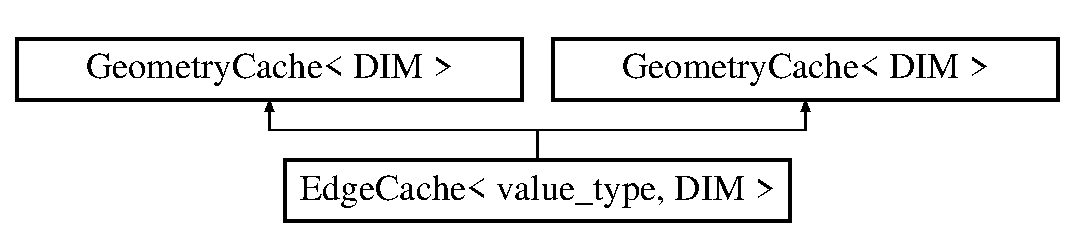
\includegraphics[height=2.000000cm]{struct_edge_cache}
\end{center}
\end{figure}
\subsection*{Public Attributes}
\begin{DoxyCompactItemize}
\item 
std\+::vector$<$ std\+::vector$<$ value\+\_\+type $>$ $>$ \mbox{\hyperlink{struct_edge_cache_a777fbadecd88c241148cfb65b30d2d2b}{basis\+\_\+value}}
\item 
std\+::vector$<$ std\+::vector$<$ std\+::vector$<$ value\+\_\+type $>$ $>$ $>$ \mbox{\hyperlink{struct_edge_cache_a2d4680a87cbdda58db97839bf250b809}{basis\+\_\+gradient}}
\item 
std\+::vector$<$ std\+::vector$<$ value\+\_\+type $>$ $>$ \mbox{\hyperlink{struct_edge_cache_a8c2a3c7fe9bb3530f6412b6c7b22d810}{un}}
\item 
u\+\_\+int \mbox{\hyperlink{struct_edge_cache_a41d2d7d840a282ed36366825d3d592b0}{idx}}
\item 
Element$<$ value\+\_\+type, \mbox{\hyperlink{complex__node___t_h_f_e_m_2uiexp_8h_a589b8b9bfdf714f736059845d568b597}{D\+IM}} $>$ $\ast$ \mbox{\hyperlink{struct_edge_cache_a35850c44237dee932b3dfa69d9a0d87d}{p\+\_\+neigh}}
\end{DoxyCompactItemize}


\subsection{Member Data Documentation}
\mbox{\Hypertarget{struct_edge_cache_a2d4680a87cbdda58db97839bf250b809}\label{struct_edge_cache_a2d4680a87cbdda58db97839bf250b809}} 
\index{Edge\+Cache@{Edge\+Cache}!basis\+\_\+gradient@{basis\+\_\+gradient}}
\index{basis\+\_\+gradient@{basis\+\_\+gradient}!Edge\+Cache@{Edge\+Cache}}
\subsubsection{\texorpdfstring{basis\+\_\+gradient}{basis\_gradient}}
{\footnotesize\ttfamily template$<$typename value\+\_\+type , int D\+IM$>$ \\
std\+::vector$<$ std\+::vector$<$ std\+::vector$<$ value\+\_\+type $>$ $>$ $>$ \mbox{\hyperlink{struct_edge_cache}{Edge\+Cache}}$<$ value\+\_\+type, \mbox{\hyperlink{complex__node___t_h_f_e_m_2uiexp_8h_a589b8b9bfdf714f736059845d568b597}{D\+IM}} $>$\+::basis\+\_\+gradient}

\mbox{\Hypertarget{struct_edge_cache_a777fbadecd88c241148cfb65b30d2d2b}\label{struct_edge_cache_a777fbadecd88c241148cfb65b30d2d2b}} 
\index{Edge\+Cache@{Edge\+Cache}!basis\+\_\+value@{basis\+\_\+value}}
\index{basis\+\_\+value@{basis\+\_\+value}!Edge\+Cache@{Edge\+Cache}}
\subsubsection{\texorpdfstring{basis\+\_\+value}{basis\_value}}
{\footnotesize\ttfamily template$<$typename value\+\_\+type , int D\+IM$>$ \\
std\+::vector$<$ std\+::vector$<$ value\+\_\+type $>$ $>$ \mbox{\hyperlink{struct_edge_cache}{Edge\+Cache}}$<$ value\+\_\+type, \mbox{\hyperlink{complex__node___t_h_f_e_m_2uiexp_8h_a589b8b9bfdf714f736059845d568b597}{D\+IM}} $>$\+::basis\+\_\+value}

\mbox{\Hypertarget{struct_edge_cache_a41d2d7d840a282ed36366825d3d592b0}\label{struct_edge_cache_a41d2d7d840a282ed36366825d3d592b0}} 
\index{Edge\+Cache@{Edge\+Cache}!idx@{idx}}
\index{idx@{idx}!Edge\+Cache@{Edge\+Cache}}
\subsubsection{\texorpdfstring{idx}{idx}}
{\footnotesize\ttfamily template$<$typename value\+\_\+type , int D\+IM$>$ \\
u\+\_\+int \mbox{\hyperlink{struct_edge_cache}{Edge\+Cache}}$<$ value\+\_\+type, \mbox{\hyperlink{complex__node___t_h_f_e_m_2uiexp_8h_a589b8b9bfdf714f736059845d568b597}{D\+IM}} $>$\+::idx}

\mbox{\Hypertarget{struct_edge_cache_a35850c44237dee932b3dfa69d9a0d87d}\label{struct_edge_cache_a35850c44237dee932b3dfa69d9a0d87d}} 
\index{Edge\+Cache@{Edge\+Cache}!p\+\_\+neigh@{p\+\_\+neigh}}
\index{p\+\_\+neigh@{p\+\_\+neigh}!Edge\+Cache@{Edge\+Cache}}
\subsubsection{\texorpdfstring{p\+\_\+neigh}{p\_neigh}}
{\footnotesize\ttfamily template$<$typename value\+\_\+type , int D\+IM$>$ \\
Element$<$value\+\_\+type,\mbox{\hyperlink{complex__node___t_h_f_e_m_2uiexp_8h_a589b8b9bfdf714f736059845d568b597}{D\+IM}}$>$$\ast$ \mbox{\hyperlink{struct_edge_cache}{Edge\+Cache}}$<$ value\+\_\+type, \mbox{\hyperlink{complex__node___t_h_f_e_m_2uiexp_8h_a589b8b9bfdf714f736059845d568b597}{D\+IM}} $>$\+::p\+\_\+neigh}

\mbox{\Hypertarget{struct_edge_cache_a8c2a3c7fe9bb3530f6412b6c7b22d810}\label{struct_edge_cache_a8c2a3c7fe9bb3530f6412b6c7b22d810}} 
\index{Edge\+Cache@{Edge\+Cache}!un@{un}}
\index{un@{un}!Edge\+Cache@{Edge\+Cache}}
\subsubsection{\texorpdfstring{un}{un}}
{\footnotesize\ttfamily template$<$typename value\+\_\+type , int D\+IM$>$ \\
std\+::vector$<$ std\+::vector$<$ value\+\_\+type $>$ $>$ \mbox{\hyperlink{struct_edge_cache}{Edge\+Cache}}$<$ value\+\_\+type, \mbox{\hyperlink{complex__node___t_h_f_e_m_2uiexp_8h_a589b8b9bfdf714f736059845d568b597}{D\+IM}} $>$\+::un}



The documentation for this struct was generated from the following file\+:\begin{DoxyCompactItemize}
\item 
complex\+\_\+edge\+\_\+\+T\+H\+F\+E\+M/\mbox{\hyperlink{complex__edge___t_h_f_e_m_2datacache_8h}{datacache.\+h}}\end{DoxyCompactItemize}

\hypertarget{struct_element_cache}{}\section{Element\+Cache$<$ value\+\_\+type, D\+IM $>$ Struct Template Reference}
\label{struct_element_cache}\index{Element\+Cache$<$ value\+\_\+type, D\+I\+M $>$@{Element\+Cache$<$ value\+\_\+type, D\+I\+M $>$}}


{\ttfamily \#include $<$datacache.\+h$>$}

Inheritance diagram for Element\+Cache$<$ value\+\_\+type, D\+IM $>$\+:\begin{figure}[H]
\begin{center}
\leavevmode
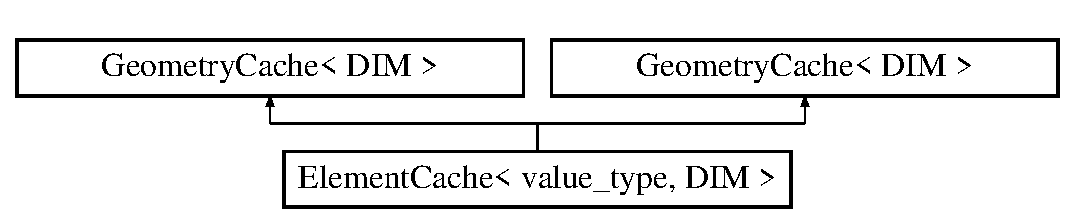
\includegraphics[height=2.000000cm]{struct_element_cache}
\end{center}
\end{figure}
\subsection*{Public Attributes}
\begin{DoxyCompactItemize}
\item 
double \mbox{\hyperlink{struct_element_cache_a285c8c9426673f094eda9254a54d358a}{ind}}
\item 
std\+::vector$<$ std\+::vector$<$ value\+\_\+type $>$ $>$ \mbox{\hyperlink{struct_element_cache_a31bc1cb436c3deb1c9aa8dad78c51a31}{basis\+\_\+value}}
\begin{DoxyCompactList}\small\item\em index of the element \end{DoxyCompactList}\item 
std\+::vector$<$ std\+::vector$<$ std\+::vector$<$ value\+\_\+type $>$ $>$ $>$ \mbox{\hyperlink{struct_element_cache_aeff46109b387c3bbcc45e2a89f387825}{basis\+\_\+gradient}}
\item 
u\+\_\+int \mbox{\hyperlink{struct_element_cache_a9f765d8abac7e3b3bb20426574404932}{idx}}
\end{DoxyCompactItemize}


\subsection{Member Data Documentation}
\mbox{\Hypertarget{struct_element_cache_aeff46109b387c3bbcc45e2a89f387825}\label{struct_element_cache_aeff46109b387c3bbcc45e2a89f387825}} 
\index{Element\+Cache@{Element\+Cache}!basis\+\_\+gradient@{basis\+\_\+gradient}}
\index{basis\+\_\+gradient@{basis\+\_\+gradient}!Element\+Cache@{Element\+Cache}}
\subsubsection{\texorpdfstring{basis\+\_\+gradient}{basis\_gradient}}
{\footnotesize\ttfamily template$<$typename value\+\_\+type , int D\+IM$>$ \\
std\+::vector$<$ std\+::vector$<$ std\+::vector$<$ value\+\_\+type $>$ $>$ $>$ \mbox{\hyperlink{struct_element_cache}{Element\+Cache}}$<$ value\+\_\+type, \mbox{\hyperlink{complex__node___t_h_f_e_m_2uiexp_8h_a589b8b9bfdf714f736059845d568b597}{D\+IM}} $>$\+::basis\+\_\+gradient}

\mbox{\Hypertarget{struct_element_cache_a31bc1cb436c3deb1c9aa8dad78c51a31}\label{struct_element_cache_a31bc1cb436c3deb1c9aa8dad78c51a31}} 
\index{Element\+Cache@{Element\+Cache}!basis\+\_\+value@{basis\+\_\+value}}
\index{basis\+\_\+value@{basis\+\_\+value}!Element\+Cache@{Element\+Cache}}
\subsubsection{\texorpdfstring{basis\+\_\+value}{basis\_value}}
{\footnotesize\ttfamily template$<$typename value\+\_\+type , int D\+IM$>$ \\
std\+::vector$<$ std\+::vector$<$ value\+\_\+type $>$ $>$ \mbox{\hyperlink{struct_element_cache}{Element\+Cache}}$<$ value\+\_\+type, \mbox{\hyperlink{complex__node___t_h_f_e_m_2uiexp_8h_a589b8b9bfdf714f736059845d568b597}{D\+IM}} $>$\+::basis\+\_\+value}



index of the element 

\mbox{\Hypertarget{struct_element_cache_a9f765d8abac7e3b3bb20426574404932}\label{struct_element_cache_a9f765d8abac7e3b3bb20426574404932}} 
\index{Element\+Cache@{Element\+Cache}!idx@{idx}}
\index{idx@{idx}!Element\+Cache@{Element\+Cache}}
\subsubsection{\texorpdfstring{idx}{idx}}
{\footnotesize\ttfamily template$<$typename value\+\_\+type , int D\+IM$>$ \\
u\+\_\+int \mbox{\hyperlink{struct_element_cache}{Element\+Cache}}$<$ value\+\_\+type, \mbox{\hyperlink{complex__node___t_h_f_e_m_2uiexp_8h_a589b8b9bfdf714f736059845d568b597}{D\+IM}} $>$\+::idx}

\mbox{\Hypertarget{struct_element_cache_a285c8c9426673f094eda9254a54d358a}\label{struct_element_cache_a285c8c9426673f094eda9254a54d358a}} 
\index{Element\+Cache@{Element\+Cache}!ind@{ind}}
\index{ind@{ind}!Element\+Cache@{Element\+Cache}}
\subsubsection{\texorpdfstring{ind}{ind}}
{\footnotesize\ttfamily template$<$typename value\+\_\+type , int D\+IM$>$ \\
double \mbox{\hyperlink{struct_element_cache}{Element\+Cache}}$<$ value\+\_\+type, \mbox{\hyperlink{complex__node___t_h_f_e_m_2uiexp_8h_a589b8b9bfdf714f736059845d568b597}{D\+IM}} $>$\+::ind}



The documentation for this struct was generated from the following file\+:\begin{DoxyCompactItemize}
\item 
complex\+\_\+edge\+\_\+\+T\+H\+F\+E\+M/\mbox{\hyperlink{complex__edge___t_h_f_e_m_2datacache_8h}{datacache.\+h}}\end{DoxyCompactItemize}

\hypertarget{struct_geometry_cache}{}\section{Geometry\+Cache$<$ D\+IM $>$ Struct Template Reference}
\label{struct_geometry_cache}\index{Geometry\+Cache$<$ D\+I\+M $>$@{Geometry\+Cache$<$ D\+I\+M $>$}}


{\ttfamily \#include $<$datacache.\+h$>$}

Inheritance diagram for Geometry\+Cache$<$ D\+IM $>$\+:\begin{figure}[H]
\begin{center}
\leavevmode
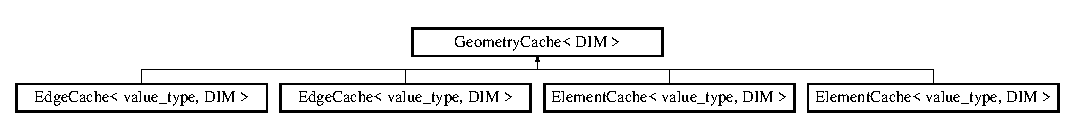
\includegraphics[height=1.278539cm]{struct_geometry_cache}
\end{center}
\end{figure}
\subsection*{Public Attributes}
\begin{DoxyCompactItemize}
\item 
Point$<$ \mbox{\hyperlink{complex__node___t_h_f_e_m_2uiexp_8h_a589b8b9bfdf714f736059845d568b597}{D\+IM}} $>$ \mbox{\hyperlink{struct_geometry_cache_a6312e0dedafa80d8a8aae0f9a99ec16d}{bc}}
\item 
int \mbox{\hyperlink{struct_geometry_cache_aa053ebb5dfb918e59595f4322d32bce6}{n\+\_\+quad\+\_\+pnt}}
\item 
std\+::vector$<$ Point$<$ \mbox{\hyperlink{complex__node___t_h_f_e_m_2uiexp_8h_a589b8b9bfdf714f736059845d568b597}{D\+IM}} $>$ $>$ \mbox{\hyperlink{struct_geometry_cache_a0af88a99d5de84b452a81e50ee60f246}{q\+\_\+pnt}}
\item 
std\+::vector$<$ double $>$ \mbox{\hyperlink{struct_geometry_cache_a31b6482011d3cc2bde276b0efce4f797}{Jxw}}
\item 
double \mbox{\hyperlink{struct_geometry_cache_ad6c7cd9d170b7fbcc819312dde144e37}{volume}}
\end{DoxyCompactItemize}


\subsection{Member Data Documentation}
\mbox{\Hypertarget{struct_geometry_cache_a6312e0dedafa80d8a8aae0f9a99ec16d}\label{struct_geometry_cache_a6312e0dedafa80d8a8aae0f9a99ec16d}} 
\index{Geometry\+Cache@{Geometry\+Cache}!bc@{bc}}
\index{bc@{bc}!Geometry\+Cache@{Geometry\+Cache}}
\subsubsection{\texorpdfstring{bc}{bc}}
{\footnotesize\ttfamily template$<$int D\+IM$>$ \\
Point$<$ \mbox{\hyperlink{complex__node___t_h_f_e_m_2uiexp_8h_a589b8b9bfdf714f736059845d568b597}{D\+IM}} $>$ \mbox{\hyperlink{struct_geometry_cache}{Geometry\+Cache}}$<$ \mbox{\hyperlink{complex__node___t_h_f_e_m_2uiexp_8h_a589b8b9bfdf714f736059845d568b597}{D\+IM}} $>$\+::bc}

\mbox{\Hypertarget{struct_geometry_cache_a31b6482011d3cc2bde276b0efce4f797}\label{struct_geometry_cache_a31b6482011d3cc2bde276b0efce4f797}} 
\index{Geometry\+Cache@{Geometry\+Cache}!Jxw@{Jxw}}
\index{Jxw@{Jxw}!Geometry\+Cache@{Geometry\+Cache}}
\subsubsection{\texorpdfstring{Jxw}{Jxw}}
{\footnotesize\ttfamily template$<$int D\+IM$>$ \\
std\+::vector$<$ double $>$ \mbox{\hyperlink{struct_geometry_cache}{Geometry\+Cache}}$<$ \mbox{\hyperlink{complex__node___t_h_f_e_m_2uiexp_8h_a589b8b9bfdf714f736059845d568b597}{D\+IM}} $>$\+::Jxw}

\mbox{\Hypertarget{struct_geometry_cache_aa053ebb5dfb918e59595f4322d32bce6}\label{struct_geometry_cache_aa053ebb5dfb918e59595f4322d32bce6}} 
\index{Geometry\+Cache@{Geometry\+Cache}!n\+\_\+quad\+\_\+pnt@{n\+\_\+quad\+\_\+pnt}}
\index{n\+\_\+quad\+\_\+pnt@{n\+\_\+quad\+\_\+pnt}!Geometry\+Cache@{Geometry\+Cache}}
\subsubsection{\texorpdfstring{n\+\_\+quad\+\_\+pnt}{n\_quad\_pnt}}
{\footnotesize\ttfamily template$<$int D\+IM$>$ \\
int \mbox{\hyperlink{struct_geometry_cache}{Geometry\+Cache}}$<$ \mbox{\hyperlink{complex__node___t_h_f_e_m_2uiexp_8h_a589b8b9bfdf714f736059845d568b597}{D\+IM}} $>$\+::n\+\_\+quad\+\_\+pnt}

\mbox{\Hypertarget{struct_geometry_cache_a0af88a99d5de84b452a81e50ee60f246}\label{struct_geometry_cache_a0af88a99d5de84b452a81e50ee60f246}} 
\index{Geometry\+Cache@{Geometry\+Cache}!q\+\_\+pnt@{q\+\_\+pnt}}
\index{q\+\_\+pnt@{q\+\_\+pnt}!Geometry\+Cache@{Geometry\+Cache}}
\subsubsection{\texorpdfstring{q\+\_\+pnt}{q\_pnt}}
{\footnotesize\ttfamily template$<$int D\+IM$>$ \\
std\+::vector$<$ Point$<$ \mbox{\hyperlink{complex__node___t_h_f_e_m_2uiexp_8h_a589b8b9bfdf714f736059845d568b597}{D\+IM}} $>$ $>$ \mbox{\hyperlink{struct_geometry_cache}{Geometry\+Cache}}$<$ \mbox{\hyperlink{complex__node___t_h_f_e_m_2uiexp_8h_a589b8b9bfdf714f736059845d568b597}{D\+IM}} $>$\+::q\+\_\+pnt}

\mbox{\Hypertarget{struct_geometry_cache_ad6c7cd9d170b7fbcc819312dde144e37}\label{struct_geometry_cache_ad6c7cd9d170b7fbcc819312dde144e37}} 
\index{Geometry\+Cache@{Geometry\+Cache}!volume@{volume}}
\index{volume@{volume}!Geometry\+Cache@{Geometry\+Cache}}
\subsubsection{\texorpdfstring{volume}{volume}}
{\footnotesize\ttfamily template$<$int D\+IM$>$ \\
double \mbox{\hyperlink{struct_geometry_cache}{Geometry\+Cache}}$<$ \mbox{\hyperlink{complex__node___t_h_f_e_m_2uiexp_8h_a589b8b9bfdf714f736059845d568b597}{D\+IM}} $>$\+::volume}



The documentation for this struct was generated from the following file\+:\begin{DoxyCompactItemize}
\item 
complex\+\_\+edge\+\_\+\+T\+H\+F\+E\+M/\mbox{\hyperlink{complex__edge___t_h_f_e_m_2datacache_8h}{datacache.\+h}}\end{DoxyCompactItemize}

\hypertarget{struct_solution_cache}{}\section{Solution\+Cache$<$ value\+\_\+type $>$ Struct Template Reference}
\label{struct_solution_cache}\index{Solution\+Cache$<$ value\+\_\+type $>$@{Solution\+Cache$<$ value\+\_\+type $>$}}


{\ttfamily \#include $<$datacache.\+h$>$}

\subsection*{Public Attributes}
\begin{DoxyCompactItemize}
\item 
std\+::vector$<$ value\+\_\+type $>$ \mbox{\hyperlink{struct_solution_cache_aa45492c5fb1bcd26f67f5e4729f9b064}{val}}
\end{DoxyCompactItemize}


\subsection{Member Data Documentation}
\mbox{\Hypertarget{struct_solution_cache_aa45492c5fb1bcd26f67f5e4729f9b064}\label{struct_solution_cache_aa45492c5fb1bcd26f67f5e4729f9b064}} 
\index{Solution\+Cache@{Solution\+Cache}!val@{val}}
\index{val@{val}!Solution\+Cache@{Solution\+Cache}}
\subsubsection{\texorpdfstring{val}{val}}
{\footnotesize\ttfamily template$<$class value\+\_\+type $>$ \\
std\+::vector$<$ value\+\_\+type $>$ \mbox{\hyperlink{struct_solution_cache}{Solution\+Cache}}$<$ value\+\_\+type $>$\+::val}



The documentation for this struct was generated from the following file\+:\begin{DoxyCompactItemize}
\item 
complex\+\_\+edge\+\_\+\+T\+H\+F\+E\+M/\mbox{\hyperlink{complex__edge___t_h_f_e_m_2datacache_8h}{datacache.\+h}}\end{DoxyCompactItemize}

\hypertarget{classui_experiment}{}\section{ui\+Experiment Class Reference}
\label{classui_experiment}\index{ui\+Experiment@{ui\+Experiment}}


{\ttfamily \#include $<$uiexp.\+h$>$}

\subsection*{Public Member Functions}
\begin{DoxyCompactItemize}
\item 
\mbox{\hyperlink{classui_experiment_aaebdbaabc4e6ab6d83015dff92519d2c}{ui\+Experiment}} (const std\+::string \&file)
\begin{DoxyCompactList}\small\item\em time step \end{DoxyCompactList}\item 
virtual \mbox{\hyperlink{classui_experiment_a1efc79d41f673a12d42211d099bbc240}{$\sim$ui\+Experiment}} ()
\item 
void \mbox{\hyperlink{classui_experiment_af19926858d11ccf9cb6a732112e381ed}{init}} ()
\item 
void \mbox{\hyperlink{classui_experiment_a82e71dbd631d00315763e0514608f0fb}{build\+F\+E\+M\+Space}} ()
\item 
void \mbox{\hyperlink{classui_experiment_a1ec010eb71e06c6388d67bbe124c951b}{build\+D\+G\+F\+E\+M\+Space}} (int bmark=2)
\item 
void \mbox{\hyperlink{classui_experiment_a406d18d100eaa0c03139590bfa6092af}{update\+Geometry\+Cache}} (u\+\_\+int alg\+\_\+acc=3)
\item 
void \mbox{\hyperlink{classui_experiment_a0c145963361c8f511360e994833a48ef}{update\+D\+G\+Geometry\+Cache}} (u\+\_\+int alg\+\_\+acc=3)
\item 
void \mbox{\hyperlink{classui_experiment_a03675f636c0949ae93bed21719f9a820}{Dirichlet\+BC}} (\mbox{\hyperlink{complex__node___t_h_f_e_m_2emdefs_8h_af8816f473dfdd972d676674921eb65f3}{C\+Func}} \mbox{\hyperlink{complex__node___t_h_f_e_m_2parameter_8h_a0150c722a481cbca4663d2d8b9a9f903}{bnd}}, int bmark=1)
\item 
void \mbox{\hyperlink{classui_experiment_ab4c24c7ae47ac21530ea765bcb970543}{Neumman\+BC}} (\mbox{\hyperlink{complex__edge___t_h_f_e_m_2emdefs_8h_ab4380503f43da11284de79277e96e96b}{Cv\+Func}} g, int bmark=2)
\item 
void \mbox{\hyperlink{classui_experiment_a1c015a570ae4f2a1c8db01275497753f}{get\+Rhs}} ()
\item 
void \mbox{\hyperlink{classui_experiment_ad09537c271da486d93b126d06e31dd2f}{get\+Mat}} ()
\item 
void \mbox{\hyperlink{classui_experiment_a542aa9e02b2ff7f40975ecce7b00a304}{solve}} ()
\item 
void \mbox{\hyperlink{classui_experiment_a4a8beb61cd0e3061d9be1273c371cadf}{get\+Error}} ()
\item 
void \mbox{\hyperlink{classui_experiment_ab560aa75b58cc9bba585adf8f6ce7d76}{adapt\+Mesh}} ()
\item 
void \mbox{\hyperlink{classui_experiment_aa01307f80d55f23738cd9ae0876280b3}{get\+Indicator}} ()
\item 
virtual void \mbox{\hyperlink{classui_experiment_a62f19f7927000e2b2b6946513917aef4}{save\+Data}} ()
\item 
void \mbox{\hyperlink{classui_experiment_aab82b5571ffb6a05e3104b7fc50ca34a}{run}} ()
\item 
\mbox{\hyperlink{classui_experiment_aaebdbaabc4e6ab6d83015dff92519d2c}{ui\+Experiment}} (const std\+::string \&file)
\begin{DoxyCompactList}\small\item\em time step \end{DoxyCompactList}\item 
virtual \mbox{\hyperlink{classui_experiment_a068797017d5804783e97385921c13253}{$\sim$ui\+Experiment}} ()
\item 
void \mbox{\hyperlink{classui_experiment_af19926858d11ccf9cb6a732112e381ed}{init}} ()
\item 
void \mbox{\hyperlink{classui_experiment_a82e71dbd631d00315763e0514608f0fb}{build\+F\+E\+M\+Space}} ()
\item 
void \mbox{\hyperlink{classui_experiment_af36eded6a690c993106e851452b52c74}{build\+D\+G\+F\+E\+M\+Space}} (int bmark=11)
\item 
void \mbox{\hyperlink{classui_experiment_a406d18d100eaa0c03139590bfa6092af}{update\+Geometry\+Cache}} (u\+\_\+int alg\+\_\+acc=3)
\item 
void \mbox{\hyperlink{classui_experiment_a0c145963361c8f511360e994833a48ef}{update\+D\+G\+Geometry\+Cache}} (u\+\_\+int alg\+\_\+acc=3)
\item 
void \mbox{\hyperlink{classui_experiment_a03675f636c0949ae93bed21719f9a820}{Dirichlet\+BC}} (\mbox{\hyperlink{complex__node___t_h_f_e_m_2emdefs_8h_af8816f473dfdd972d676674921eb65f3}{C\+Func}} \mbox{\hyperlink{complex__node___t_h_f_e_m_2parameter_8h_a0150c722a481cbca4663d2d8b9a9f903}{bnd}}, int bmark=1)
\item 
void \mbox{\hyperlink{classui_experiment_afd027bbfa6350cfb77a0208721c56ebe}{Neumman\+BC}} (\mbox{\hyperlink{complex__node___t_h_f_e_m_2emdefs_8h_af8816f473dfdd972d676674921eb65f3}{C\+Func}} g, int bmark=11)
\item 
void \mbox{\hyperlink{classui_experiment_a1c015a570ae4f2a1c8db01275497753f}{get\+Rhs}} ()
\item 
void \mbox{\hyperlink{classui_experiment_ad09537c271da486d93b126d06e31dd2f}{get\+Mat}} ()
\item 
void \mbox{\hyperlink{classui_experiment_a542aa9e02b2ff7f40975ecce7b00a304}{solve}} ()
\item 
void \mbox{\hyperlink{classui_experiment_a4a8beb61cd0e3061d9be1273c371cadf}{get\+Error}} ()
\item 
void \mbox{\hyperlink{classui_experiment_ab560aa75b58cc9bba585adf8f6ce7d76}{adapt\+Mesh}} ()
\item 
void \mbox{\hyperlink{classui_experiment_aa01307f80d55f23738cd9ae0876280b3}{get\+Indicator}} ()
\item 
virtual void \mbox{\hyperlink{classui_experiment_a1b08fa8cc473ac030f73bcc46048cf45}{save\+Data}} ()
\item 
void \mbox{\hyperlink{classui_experiment_aab82b5571ffb6a05e3104b7fc50ca34a}{run}} ()
\end{DoxyCompactItemize}
\subsection*{Private Attributes}
\begin{DoxyCompactItemize}
\item 
H\+Geometry\+Tree$<$ \mbox{\hyperlink{complex__node___t_h_f_e_m_2uiexp_8h_a589b8b9bfdf714f736059845d568b597}{D\+IM}} $>$ \mbox{\hyperlink{classui_experiment_a7b3828699381e953e413984d65c27c76}{h\+\_\+tree}}
\item 
Irregular\+Mesh$<$ \mbox{\hyperlink{complex__node___t_h_f_e_m_2uiexp_8h_a589b8b9bfdf714f736059845d568b597}{D\+IM}} $>$ \mbox{\hyperlink{classui_experiment_a51e99f27dde8abd769e217d8192b1953}{ir\+\_\+mesh}}
\item 
std\+::string \mbox{\hyperlink{classui_experiment_ad22a4c3bcc758175bee8a9cc6112c37b}{mesh\+\_\+file}}
\item 
Template\+Geometry$<$ \mbox{\hyperlink{complex__node___t_h_f_e_m_2uiexp_8h_a589b8b9bfdf714f736059845d568b597}{D\+IM}} $>$ \mbox{\hyperlink{classui_experiment_a2c9abfb62147cb378fd5a7f52e99560e}{triangle\+\_\+template\+\_\+geometry}}
\begin{DoxyCompactList}\small\item\em mesh file \end{DoxyCompactList}\item 
Coord\+Transform$<$ \mbox{\hyperlink{complex__node___t_h_f_e_m_2uiexp_8h_a589b8b9bfdf714f736059845d568b597}{D\+IM}}, \mbox{\hyperlink{complex__node___t_h_f_e_m_2uiexp_8h_a589b8b9bfdf714f736059845d568b597}{D\+IM}} $>$ \mbox{\hyperlink{classui_experiment_a83ec25f4aedfaca2d4878b15efc82315}{triangle\+\_\+coord\+\_\+transform}}
\item 
Template\+D\+OF$<$ \mbox{\hyperlink{complex__node___t_h_f_e_m_2uiexp_8h_a589b8b9bfdf714f736059845d568b597}{D\+IM}} $>$ \mbox{\hyperlink{classui_experiment_a513ca14667fb30909ea3aef90e13200c}{triangle\+\_\+template\+\_\+dof}}
\item 
Basis\+Function\+Admin$<$ \mbox{\hyperlink{complex__edge___t_h_f_e_m_2emdefs_8h_a0a0de407de54661e0d56aa8686c104d9}{vec\+\_\+type}}, \mbox{\hyperlink{complex__node___t_h_f_e_m_2uiexp_8h_a589b8b9bfdf714f736059845d568b597}{D\+IM}}, \mbox{\hyperlink{complex__node___t_h_f_e_m_2uiexp_8h_a589b8b9bfdf714f736059845d568b597}{D\+IM}} $>$ \mbox{\hyperlink{classui_experiment_a4afff2bbca9b68fe61856dcf07456d2c}{triangle\+\_\+basis\+\_\+function}}
\item 
Unit\+Out\+Normal$<$ \mbox{\hyperlink{complex__node___t_h_f_e_m_2uiexp_8h_a589b8b9bfdf714f736059845d568b597}{D\+IM}} $>$ \mbox{\hyperlink{classui_experiment_a5105926d18f9fc118426f833b63fbec6}{triangle\+\_\+unit\+\_\+out\+\_\+normal}}
\item 
Template\+Geometry$<$ \mbox{\hyperlink{complex__node___t_h_f_e_m_2uiexp_8h_a589b8b9bfdf714f736059845d568b597}{D\+IM}} $>$ \mbox{\hyperlink{classui_experiment_a880d54a1384f86b7bacc8dfb476a20e6}{twin\+\_\+triangle\+\_\+template\+\_\+geometry}}
\item 
Coord\+Transform$<$ \mbox{\hyperlink{complex__node___t_h_f_e_m_2uiexp_8h_a589b8b9bfdf714f736059845d568b597}{D\+IM}}, \mbox{\hyperlink{complex__node___t_h_f_e_m_2uiexp_8h_a589b8b9bfdf714f736059845d568b597}{D\+IM}} $>$ \mbox{\hyperlink{classui_experiment_a6607a6e91fd6cd91332f6cda9964193f}{twin\+\_\+triangle\+\_\+coord\+\_\+transform}}
\item 
Template\+D\+OF$<$ \mbox{\hyperlink{complex__node___t_h_f_e_m_2uiexp_8h_a589b8b9bfdf714f736059845d568b597}{D\+IM}} $>$ \mbox{\hyperlink{classui_experiment_a4f54e2b65f1b693be17259d4ec19e93b}{twin\+\_\+triangle\+\_\+template\+\_\+dof}}
\item 
Basis\+Function\+Admin$<$ \mbox{\hyperlink{complex__edge___t_h_f_e_m_2emdefs_8h_a0a0de407de54661e0d56aa8686c104d9}{vec\+\_\+type}}, \mbox{\hyperlink{complex__node___t_h_f_e_m_2uiexp_8h_a589b8b9bfdf714f736059845d568b597}{D\+IM}}, \mbox{\hyperlink{complex__node___t_h_f_e_m_2uiexp_8h_a589b8b9bfdf714f736059845d568b597}{D\+IM}} $>$ \mbox{\hyperlink{classui_experiment_ab2decc2422c7eac7248bb615f629b312}{twin\+\_\+triangle\+\_\+basis\+\_\+function}}
\item 
Unit\+Out\+Normal$<$ \mbox{\hyperlink{complex__node___t_h_f_e_m_2uiexp_8h_a589b8b9bfdf714f736059845d568b597}{D\+IM}} $>$ \mbox{\hyperlink{classui_experiment_a3240a812867c50cd296cff62e86731d5}{twin\+\_\+triangle\+\_\+unit\+\_\+out\+\_\+normal}}
\item 
Template\+Geometry$<$ \mbox{\hyperlink{complex__node___t_h_f_e_m_2uiexp_8h_a589b8b9bfdf714f736059845d568b597}{D\+IM}}-\/1 $>$ \mbox{\hyperlink{classui_experiment_a604866b155caa1e05fa9e23f37822885}{interval\+\_\+template\+\_\+geometry}}
\item 
Coord\+Transform$<$ \mbox{\hyperlink{complex__node___t_h_f_e_m_2uiexp_8h_a589b8b9bfdf714f736059845d568b597}{D\+IM}}-\/1, \mbox{\hyperlink{complex__node___t_h_f_e_m_2uiexp_8h_a589b8b9bfdf714f736059845d568b597}{D\+IM}} $>$ \mbox{\hyperlink{classui_experiment_a58e8bc2ca812d734691af34491626d5b}{interval\+\_\+to2d\+\_\+coord\+\_\+transform}}
\item 
std\+::vector$<$ Template\+Element$<$ \mbox{\hyperlink{complex__edge___t_h_f_e_m_2emdefs_8h_a0a0de407de54661e0d56aa8686c104d9}{vec\+\_\+type}}, \mbox{\hyperlink{complex__node___t_h_f_e_m_2uiexp_8h_a589b8b9bfdf714f736059845d568b597}{D\+IM}}, \mbox{\hyperlink{complex__node___t_h_f_e_m_2uiexp_8h_a589b8b9bfdf714f736059845d568b597}{D\+IM}} $>$ $>$ \mbox{\hyperlink{classui_experiment_a9716ddbac22d7311f919fe55991e8930}{template\+\_\+element}}
\item 
std\+::vector$<$ Template\+D\+G\+Element$<$ \mbox{\hyperlink{complex__node___t_h_f_e_m_2uiexp_8h_a589b8b9bfdf714f736059845d568b597}{D\+IM}}-\/1, \mbox{\hyperlink{complex__node___t_h_f_e_m_2uiexp_8h_a589b8b9bfdf714f736059845d568b597}{D\+IM}} $>$ $>$ \mbox{\hyperlink{classui_experiment_ac5384376bf5ff36cb3d5784876972f4d}{dg\+\_\+template\+\_\+element}}
\item 
D\+G\+F\+E\+M\+Space$<$ \mbox{\hyperlink{complex__edge___t_h_f_e_m_2emdefs_8h_a0a0de407de54661e0d56aa8686c104d9}{vec\+\_\+type}}, \mbox{\hyperlink{complex__node___t_h_f_e_m_2uiexp_8h_a589b8b9bfdf714f736059845d568b597}{D\+IM}} $>$ \mbox{\hyperlink{classui_experiment_ad4b0994c9d2bd5691065434080468700}{fem\+\_\+space}}
\item 
std\+::vector$<$ \mbox{\hyperlink{struct_element_cache}{Element\+Cache}}$<$ \mbox{\hyperlink{complex__edge___t_h_f_e_m_2emdefs_8h_a0a0de407de54661e0d56aa8686c104d9}{vec\+\_\+type}}, \mbox{\hyperlink{complex__node___t_h_f_e_m_2uiexp_8h_a589b8b9bfdf714f736059845d568b597}{D\+IM}} $>$ $>$ \mbox{\hyperlink{classui_experiment_a86da24faea838d0a39a7b89d2f09c81c}{element\+\_\+cache}}
\begin{DoxyCompactList}\small\item\em finite element space \end{DoxyCompactList}\item 
std\+::vector$<$ \mbox{\hyperlink{struct_edge_cache}{Edge\+Cache}}$<$ double, \mbox{\hyperlink{complex__node___t_h_f_e_m_2uiexp_8h_a589b8b9bfdf714f736059845d568b597}{D\+IM}} $>$ $>$ \mbox{\hyperlink{classui_experiment_a8c9962fa5c8eefe78f7d0612e0fd7dd2}{edge\+\_\+cache}}
\item 
F\+E\+M\+Function$<$ \mbox{\hyperlink{complex__edge___t_h_f_e_m_2emdefs_8h_a0a0de407de54661e0d56aa8686c104d9}{vec\+\_\+type}}, \mbox{\hyperlink{complex__node___t_h_f_e_m_2uiexp_8h_a589b8b9bfdf714f736059845d568b597}{D\+IM}} $>$ \mbox{\hyperlink{classui_experiment_aabad5b9464e03403d9c443b5130325f9}{u\+\_\+re}}
\item 
F\+E\+M\+Function$<$ \mbox{\hyperlink{complex__edge___t_h_f_e_m_2emdefs_8h_a0a0de407de54661e0d56aa8686c104d9}{vec\+\_\+type}}, \mbox{\hyperlink{complex__node___t_h_f_e_m_2uiexp_8h_a589b8b9bfdf714f736059845d568b597}{D\+IM}} $>$ \mbox{\hyperlink{classui_experiment_aa50bc0a5012bc931d4d42ca06c303a45}{u\+\_\+im}}
\item 
Eigen\+::\+Sparse\+Matrix$<$ \mbox{\hyperlink{complex__edge___t_h_f_e_m_2emdefs_8h_a97d2dbb382a9b25c16c04fc1e1baacdb}{cvaltype}}, Eigen\+::\+Row\+Major $>$ \mbox{\hyperlink{classui_experiment_a8e554eb0972c60b11ee11dc44753ae97}{stiff\+\_\+matrix}}
\item 
Eigen\+::\+Matrix$<$ \mbox{\hyperlink{complex__edge___t_h_f_e_m_2emdefs_8h_a97d2dbb382a9b25c16c04fc1e1baacdb}{cvaltype}}, Eigen\+::\+Dynamic, 1 $>$ \mbox{\hyperlink{classui_experiment_aaf0657e489f16f47ecf61b4bc0051648}{solution}}
\item 
Eigen\+::\+Matrix$<$ \mbox{\hyperlink{complex__edge___t_h_f_e_m_2emdefs_8h_a97d2dbb382a9b25c16c04fc1e1baacdb}{cvaltype}}, Eigen\+::\+Dynamic, 1 $>$ \mbox{\hyperlink{classui_experiment_a0d42caa6e050d49531d7d006efbef6a8}{rhs}}
\item 
std\+::vector$<$ \mbox{\hyperlink{complex__edge___t_h_f_e_m_2uiexp_8h_a8014ab9a69eccab08613f4642bbbddd5}{T}} $>$ \mbox{\hyperlink{classui_experiment_adc77b528327a0ac71f395005b2008568}{triplets}}
\item 
Indicator$<$ \mbox{\hyperlink{complex__node___t_h_f_e_m_2uiexp_8h_a589b8b9bfdf714f736059845d568b597}{D\+IM}} $>$ \mbox{\hyperlink{classui_experiment_a8400becec774a3accdec7f0e7a102cbd}{indicator}}
\item 
Mesh\+Adaptor$<$ \mbox{\hyperlink{complex__node___t_h_f_e_m_2uiexp_8h_a589b8b9bfdf714f736059845d568b597}{D\+IM}} $>$ \mbox{\hyperlink{classui_experiment_a3043c4d1d53dc7026d83398b7caa2010}{mesh\+\_\+adaptor}}
\item 
double \mbox{\hyperlink{classui_experiment_ab2f282868b75fb348ac4c99d2d84441e}{sys\+\_\+t0}} = 0
\item 
double \mbox{\hyperlink{classui_experiment_a636bedd4cd6e21255631fbaa556427f2}{dt}} = 1
\begin{DoxyCompactList}\small\item\em system start time \end{DoxyCompactList}\item 
Basis\+Function\+Admin$<$ double, \mbox{\hyperlink{complex__node___t_h_f_e_m_2uiexp_8h_a589b8b9bfdf714f736059845d568b597}{D\+IM}}, \mbox{\hyperlink{complex__node___t_h_f_e_m_2uiexp_8h_a589b8b9bfdf714f736059845d568b597}{D\+IM}} $>$ \mbox{\hyperlink{classui_experiment_a9877c48b948d57a73663d4b3a741d6ae}{triangle\+\_\+basis\+\_\+function}}
\item 
Basis\+Function\+Admin$<$ double, \mbox{\hyperlink{complex__node___t_h_f_e_m_2uiexp_8h_a589b8b9bfdf714f736059845d568b597}{D\+IM}}, \mbox{\hyperlink{complex__node___t_h_f_e_m_2uiexp_8h_a589b8b9bfdf714f736059845d568b597}{D\+IM}} $>$ \mbox{\hyperlink{classui_experiment_a20934ca922429d4b15fb94830a1475f1}{twin\+\_\+triangle\+\_\+basis\+\_\+function}}
\item 
std\+::vector$<$ Template\+Element$<$ double, \mbox{\hyperlink{complex__node___t_h_f_e_m_2uiexp_8h_a589b8b9bfdf714f736059845d568b597}{D\+IM}}, \mbox{\hyperlink{complex__node___t_h_f_e_m_2uiexp_8h_a589b8b9bfdf714f736059845d568b597}{D\+IM}} $>$ $>$ \mbox{\hyperlink{classui_experiment_a7706058764736bd2091122372d448c78}{template\+\_\+element}}
\item 
D\+G\+F\+E\+M\+Space$<$ double, \mbox{\hyperlink{complex__node___t_h_f_e_m_2uiexp_8h_a589b8b9bfdf714f736059845d568b597}{D\+IM}} $>$ \mbox{\hyperlink{classui_experiment_a7532fa0202196a17b46ea8a3c9241410}{fem\+\_\+space}}
\item 
std\+::vector$<$ \mbox{\hyperlink{struct_element_cache}{Element\+Cache}}$<$ double, \mbox{\hyperlink{complex__node___t_h_f_e_m_2uiexp_8h_a589b8b9bfdf714f736059845d568b597}{D\+IM}} $>$ $>$ \mbox{\hyperlink{classui_experiment_a3386a72dec8a1d7065f553f42d1f181b}{element\+\_\+cache}}
\begin{DoxyCompactList}\small\item\em finite element space \end{DoxyCompactList}\item 
F\+E\+M\+Function$<$ double, \mbox{\hyperlink{complex__node___t_h_f_e_m_2uiexp_8h_a589b8b9bfdf714f736059845d568b597}{D\+IM}} $>$ \mbox{\hyperlink{classui_experiment_aac4bf7e51a978a58d1dab5f0dcb62b54}{u\+\_\+re}}
\item 
F\+E\+M\+Function$<$ double, \mbox{\hyperlink{complex__node___t_h_f_e_m_2uiexp_8h_a589b8b9bfdf714f736059845d568b597}{D\+IM}} $>$ \mbox{\hyperlink{classui_experiment_a52c236e8afbb37ae0baa97ada2305d93}{u\+\_\+im}}
\end{DoxyCompactItemize}


\subsection{Constructor \& Destructor Documentation}
\mbox{\Hypertarget{classui_experiment_aaebdbaabc4e6ab6d83015dff92519d2c}\label{classui_experiment_aaebdbaabc4e6ab6d83015dff92519d2c}} 
\index{ui\+Experiment@{ui\+Experiment}!ui\+Experiment@{ui\+Experiment}}
\index{ui\+Experiment@{ui\+Experiment}!ui\+Experiment@{ui\+Experiment}}
\subsubsection{\texorpdfstring{ui\+Experiment()}{uiExperiment()}\hspace{0.1cm}{\footnotesize\ttfamily [1/2]}}
{\footnotesize\ttfamily ui\+Experiment\+::ui\+Experiment (\begin{DoxyParamCaption}\item[{const std\+::string \&}]{file }\end{DoxyParamCaption})}



time step 

\mbox{\Hypertarget{classui_experiment_a1efc79d41f673a12d42211d099bbc240}\label{classui_experiment_a1efc79d41f673a12d42211d099bbc240}} 
\index{ui\+Experiment@{ui\+Experiment}!````~ui\+Experiment@{$\sim$ui\+Experiment}}
\index{````~ui\+Experiment@{$\sim$ui\+Experiment}!ui\+Experiment@{ui\+Experiment}}
\subsubsection{\texorpdfstring{$\sim$ui\+Experiment()}{~uiExperiment()}\hspace{0.1cm}{\footnotesize\ttfamily [1/2]}}
{\footnotesize\ttfamily ui\+Experiment\+::$\sim$ui\+Experiment (\begin{DoxyParamCaption}{ }\end{DoxyParamCaption})\hspace{0.3cm}{\ttfamily [virtual]}}

\mbox{\Hypertarget{classui_experiment_aaebdbaabc4e6ab6d83015dff92519d2c}\label{classui_experiment_aaebdbaabc4e6ab6d83015dff92519d2c}} 
\index{ui\+Experiment@{ui\+Experiment}!ui\+Experiment@{ui\+Experiment}}
\index{ui\+Experiment@{ui\+Experiment}!ui\+Experiment@{ui\+Experiment}}
\subsubsection{\texorpdfstring{ui\+Experiment()}{uiExperiment()}\hspace{0.1cm}{\footnotesize\ttfamily [2/2]}}
{\footnotesize\ttfamily ui\+Experiment\+::ui\+Experiment (\begin{DoxyParamCaption}\item[{const std\+::string \&}]{file }\end{DoxyParamCaption})}



time step 

\mbox{\Hypertarget{classui_experiment_a068797017d5804783e97385921c13253}\label{classui_experiment_a068797017d5804783e97385921c13253}} 
\index{ui\+Experiment@{ui\+Experiment}!````~ui\+Experiment@{$\sim$ui\+Experiment}}
\index{````~ui\+Experiment@{$\sim$ui\+Experiment}!ui\+Experiment@{ui\+Experiment}}
\subsubsection{\texorpdfstring{$\sim$ui\+Experiment()}{~uiExperiment()}\hspace{0.1cm}{\footnotesize\ttfamily [2/2]}}
{\footnotesize\ttfamily virtual ui\+Experiment\+::$\sim$ui\+Experiment (\begin{DoxyParamCaption}{ }\end{DoxyParamCaption})\hspace{0.3cm}{\ttfamily [virtual]}}



\subsection{Member Function Documentation}
\mbox{\Hypertarget{classui_experiment_ab560aa75b58cc9bba585adf8f6ce7d76}\label{classui_experiment_ab560aa75b58cc9bba585adf8f6ce7d76}} 
\index{ui\+Experiment@{ui\+Experiment}!adapt\+Mesh@{adapt\+Mesh}}
\index{adapt\+Mesh@{adapt\+Mesh}!ui\+Experiment@{ui\+Experiment}}
\subsubsection{\texorpdfstring{adapt\+Mesh()}{adaptMesh()}\hspace{0.1cm}{\footnotesize\ttfamily [1/2]}}
{\footnotesize\ttfamily void ui\+Experiment\+::adapt\+Mesh (\begin{DoxyParamCaption}{ }\end{DoxyParamCaption})}

\mbox{\Hypertarget{classui_experiment_ab560aa75b58cc9bba585adf8f6ce7d76}\label{classui_experiment_ab560aa75b58cc9bba585adf8f6ce7d76}} 
\index{ui\+Experiment@{ui\+Experiment}!adapt\+Mesh@{adapt\+Mesh}}
\index{adapt\+Mesh@{adapt\+Mesh}!ui\+Experiment@{ui\+Experiment}}
\subsubsection{\texorpdfstring{adapt\+Mesh()}{adaptMesh()}\hspace{0.1cm}{\footnotesize\ttfamily [2/2]}}
{\footnotesize\ttfamily void ui\+Experiment\+::adapt\+Mesh (\begin{DoxyParamCaption}{ }\end{DoxyParamCaption})}

\mbox{\Hypertarget{classui_experiment_a1ec010eb71e06c6388d67bbe124c951b}\label{classui_experiment_a1ec010eb71e06c6388d67bbe124c951b}} 
\index{ui\+Experiment@{ui\+Experiment}!build\+D\+G\+F\+E\+M\+Space@{build\+D\+G\+F\+E\+M\+Space}}
\index{build\+D\+G\+F\+E\+M\+Space@{build\+D\+G\+F\+E\+M\+Space}!ui\+Experiment@{ui\+Experiment}}
\subsubsection{\texorpdfstring{build\+D\+G\+F\+E\+M\+Space()}{buildDGFEMSpace()}\hspace{0.1cm}{\footnotesize\ttfamily [1/2]}}
{\footnotesize\ttfamily void ui\+Experiment\+::build\+D\+G\+F\+E\+M\+Space (\begin{DoxyParamCaption}\item[{int}]{bmark = {\ttfamily 2} }\end{DoxyParamCaption})}

\mbox{\Hypertarget{classui_experiment_af36eded6a690c993106e851452b52c74}\label{classui_experiment_af36eded6a690c993106e851452b52c74}} 
\index{ui\+Experiment@{ui\+Experiment}!build\+D\+G\+F\+E\+M\+Space@{build\+D\+G\+F\+E\+M\+Space}}
\index{build\+D\+G\+F\+E\+M\+Space@{build\+D\+G\+F\+E\+M\+Space}!ui\+Experiment@{ui\+Experiment}}
\subsubsection{\texorpdfstring{build\+D\+G\+F\+E\+M\+Space()}{buildDGFEMSpace()}\hspace{0.1cm}{\footnotesize\ttfamily [2/2]}}
{\footnotesize\ttfamily void ui\+Experiment\+::build\+D\+G\+F\+E\+M\+Space (\begin{DoxyParamCaption}\item[{int}]{bmark = {\ttfamily 11} }\end{DoxyParamCaption})}

\mbox{\Hypertarget{classui_experiment_a82e71dbd631d00315763e0514608f0fb}\label{classui_experiment_a82e71dbd631d00315763e0514608f0fb}} 
\index{ui\+Experiment@{ui\+Experiment}!build\+F\+E\+M\+Space@{build\+F\+E\+M\+Space}}
\index{build\+F\+E\+M\+Space@{build\+F\+E\+M\+Space}!ui\+Experiment@{ui\+Experiment}}
\subsubsection{\texorpdfstring{build\+F\+E\+M\+Space()}{buildFEMSpace()}\hspace{0.1cm}{\footnotesize\ttfamily [1/2]}}
{\footnotesize\ttfamily void ui\+Experiment\+::build\+F\+E\+M\+Space (\begin{DoxyParamCaption}{ }\end{DoxyParamCaption})}

\mbox{\Hypertarget{classui_experiment_a82e71dbd631d00315763e0514608f0fb}\label{classui_experiment_a82e71dbd631d00315763e0514608f0fb}} 
\index{ui\+Experiment@{ui\+Experiment}!build\+F\+E\+M\+Space@{build\+F\+E\+M\+Space}}
\index{build\+F\+E\+M\+Space@{build\+F\+E\+M\+Space}!ui\+Experiment@{ui\+Experiment}}
\subsubsection{\texorpdfstring{build\+F\+E\+M\+Space()}{buildFEMSpace()}\hspace{0.1cm}{\footnotesize\ttfamily [2/2]}}
{\footnotesize\ttfamily void ui\+Experiment\+::build\+F\+E\+M\+Space (\begin{DoxyParamCaption}{ }\end{DoxyParamCaption})}

\mbox{\Hypertarget{classui_experiment_a03675f636c0949ae93bed21719f9a820}\label{classui_experiment_a03675f636c0949ae93bed21719f9a820}} 
\index{ui\+Experiment@{ui\+Experiment}!Dirichlet\+BC@{Dirichlet\+BC}}
\index{Dirichlet\+BC@{Dirichlet\+BC}!ui\+Experiment@{ui\+Experiment}}
\subsubsection{\texorpdfstring{Dirichlet\+B\+C()}{DirichletBC()}\hspace{0.1cm}{\footnotesize\ttfamily [1/2]}}
{\footnotesize\ttfamily void ui\+Experiment\+::\+Dirichlet\+BC (\begin{DoxyParamCaption}\item[{\mbox{\hyperlink{complex__node___t_h_f_e_m_2emdefs_8h_af8816f473dfdd972d676674921eb65f3}{C\+Func}}}]{bnd,  }\item[{int}]{bmark = {\ttfamily 1} }\end{DoxyParamCaption})}

\mbox{\Hypertarget{classui_experiment_a03675f636c0949ae93bed21719f9a820}\label{classui_experiment_a03675f636c0949ae93bed21719f9a820}} 
\index{ui\+Experiment@{ui\+Experiment}!Dirichlet\+BC@{Dirichlet\+BC}}
\index{Dirichlet\+BC@{Dirichlet\+BC}!ui\+Experiment@{ui\+Experiment}}
\subsubsection{\texorpdfstring{Dirichlet\+B\+C()}{DirichletBC()}\hspace{0.1cm}{\footnotesize\ttfamily [2/2]}}
{\footnotesize\ttfamily void ui\+Experiment\+::\+Dirichlet\+BC (\begin{DoxyParamCaption}\item[{\mbox{\hyperlink{complex__node___t_h_f_e_m_2emdefs_8h_af8816f473dfdd972d676674921eb65f3}{C\+Func}}}]{bnd,  }\item[{int}]{bmark = {\ttfamily 1} }\end{DoxyParamCaption})}

\mbox{\Hypertarget{classui_experiment_a4a8beb61cd0e3061d9be1273c371cadf}\label{classui_experiment_a4a8beb61cd0e3061d9be1273c371cadf}} 
\index{ui\+Experiment@{ui\+Experiment}!get\+Error@{get\+Error}}
\index{get\+Error@{get\+Error}!ui\+Experiment@{ui\+Experiment}}
\subsubsection{\texorpdfstring{get\+Error()}{getError()}\hspace{0.1cm}{\footnotesize\ttfamily [1/2]}}
{\footnotesize\ttfamily void ui\+Experiment\+::get\+Error (\begin{DoxyParamCaption}{ }\end{DoxyParamCaption})}

\mbox{\Hypertarget{classui_experiment_a4a8beb61cd0e3061d9be1273c371cadf}\label{classui_experiment_a4a8beb61cd0e3061d9be1273c371cadf}} 
\index{ui\+Experiment@{ui\+Experiment}!get\+Error@{get\+Error}}
\index{get\+Error@{get\+Error}!ui\+Experiment@{ui\+Experiment}}
\subsubsection{\texorpdfstring{get\+Error()}{getError()}\hspace{0.1cm}{\footnotesize\ttfamily [2/2]}}
{\footnotesize\ttfamily void ui\+Experiment\+::get\+Error (\begin{DoxyParamCaption}{ }\end{DoxyParamCaption})}

\mbox{\Hypertarget{classui_experiment_aa01307f80d55f23738cd9ae0876280b3}\label{classui_experiment_aa01307f80d55f23738cd9ae0876280b3}} 
\index{ui\+Experiment@{ui\+Experiment}!get\+Indicator@{get\+Indicator}}
\index{get\+Indicator@{get\+Indicator}!ui\+Experiment@{ui\+Experiment}}
\subsubsection{\texorpdfstring{get\+Indicator()}{getIndicator()}\hspace{0.1cm}{\footnotesize\ttfamily [1/2]}}
{\footnotesize\ttfamily void ui\+Experiment\+::get\+Indicator (\begin{DoxyParamCaption}{ }\end{DoxyParamCaption})}

\mbox{\Hypertarget{classui_experiment_aa01307f80d55f23738cd9ae0876280b3}\label{classui_experiment_aa01307f80d55f23738cd9ae0876280b3}} 
\index{ui\+Experiment@{ui\+Experiment}!get\+Indicator@{get\+Indicator}}
\index{get\+Indicator@{get\+Indicator}!ui\+Experiment@{ui\+Experiment}}
\subsubsection{\texorpdfstring{get\+Indicator()}{getIndicator()}\hspace{0.1cm}{\footnotesize\ttfamily [2/2]}}
{\footnotesize\ttfamily void ui\+Experiment\+::get\+Indicator (\begin{DoxyParamCaption}{ }\end{DoxyParamCaption})}

\mbox{\Hypertarget{classui_experiment_ad09537c271da486d93b126d06e31dd2f}\label{classui_experiment_ad09537c271da486d93b126d06e31dd2f}} 
\index{ui\+Experiment@{ui\+Experiment}!get\+Mat@{get\+Mat}}
\index{get\+Mat@{get\+Mat}!ui\+Experiment@{ui\+Experiment}}
\subsubsection{\texorpdfstring{get\+Mat()}{getMat()}\hspace{0.1cm}{\footnotesize\ttfamily [1/2]}}
{\footnotesize\ttfamily void ui\+Experiment\+::get\+Mat (\begin{DoxyParamCaption}{ }\end{DoxyParamCaption})}

\mbox{\Hypertarget{classui_experiment_ad09537c271da486d93b126d06e31dd2f}\label{classui_experiment_ad09537c271da486d93b126d06e31dd2f}} 
\index{ui\+Experiment@{ui\+Experiment}!get\+Mat@{get\+Mat}}
\index{get\+Mat@{get\+Mat}!ui\+Experiment@{ui\+Experiment}}
\subsubsection{\texorpdfstring{get\+Mat()}{getMat()}\hspace{0.1cm}{\footnotesize\ttfamily [2/2]}}
{\footnotesize\ttfamily void ui\+Experiment\+::get\+Mat (\begin{DoxyParamCaption}{ }\end{DoxyParamCaption})}

\mbox{\Hypertarget{classui_experiment_a1c015a570ae4f2a1c8db01275497753f}\label{classui_experiment_a1c015a570ae4f2a1c8db01275497753f}} 
\index{ui\+Experiment@{ui\+Experiment}!get\+Rhs@{get\+Rhs}}
\index{get\+Rhs@{get\+Rhs}!ui\+Experiment@{ui\+Experiment}}
\subsubsection{\texorpdfstring{get\+Rhs()}{getRhs()}\hspace{0.1cm}{\footnotesize\ttfamily [1/2]}}
{\footnotesize\ttfamily void ui\+Experiment\+::get\+Rhs (\begin{DoxyParamCaption}{ }\end{DoxyParamCaption})}

\mbox{\Hypertarget{classui_experiment_a1c015a570ae4f2a1c8db01275497753f}\label{classui_experiment_a1c015a570ae4f2a1c8db01275497753f}} 
\index{ui\+Experiment@{ui\+Experiment}!get\+Rhs@{get\+Rhs}}
\index{get\+Rhs@{get\+Rhs}!ui\+Experiment@{ui\+Experiment}}
\subsubsection{\texorpdfstring{get\+Rhs()}{getRhs()}\hspace{0.1cm}{\footnotesize\ttfamily [2/2]}}
{\footnotesize\ttfamily void ui\+Experiment\+::get\+Rhs (\begin{DoxyParamCaption}{ }\end{DoxyParamCaption})}

\mbox{\Hypertarget{classui_experiment_af19926858d11ccf9cb6a732112e381ed}\label{classui_experiment_af19926858d11ccf9cb6a732112e381ed}} 
\index{ui\+Experiment@{ui\+Experiment}!init@{init}}
\index{init@{init}!ui\+Experiment@{ui\+Experiment}}
\subsubsection{\texorpdfstring{init()}{init()}\hspace{0.1cm}{\footnotesize\ttfamily [1/2]}}
{\footnotesize\ttfamily void ui\+Experiment\+::init (\begin{DoxyParamCaption}{ }\end{DoxyParamCaption})}

\mbox{\Hypertarget{classui_experiment_af19926858d11ccf9cb6a732112e381ed}\label{classui_experiment_af19926858d11ccf9cb6a732112e381ed}} 
\index{ui\+Experiment@{ui\+Experiment}!init@{init}}
\index{init@{init}!ui\+Experiment@{ui\+Experiment}}
\subsubsection{\texorpdfstring{init()}{init()}\hspace{0.1cm}{\footnotesize\ttfamily [2/2]}}
{\footnotesize\ttfamily void ui\+Experiment\+::init (\begin{DoxyParamCaption}{ }\end{DoxyParamCaption})}

\mbox{\Hypertarget{classui_experiment_ab4c24c7ae47ac21530ea765bcb970543}\label{classui_experiment_ab4c24c7ae47ac21530ea765bcb970543}} 
\index{ui\+Experiment@{ui\+Experiment}!Neumman\+BC@{Neumman\+BC}}
\index{Neumman\+BC@{Neumman\+BC}!ui\+Experiment@{ui\+Experiment}}
\subsubsection{\texorpdfstring{Neumman\+B\+C()}{NeummanBC()}\hspace{0.1cm}{\footnotesize\ttfamily [1/2]}}
{\footnotesize\ttfamily void ui\+Experiment\+::\+Neumman\+BC (\begin{DoxyParamCaption}\item[{\mbox{\hyperlink{complex__edge___t_h_f_e_m_2emdefs_8h_ab4380503f43da11284de79277e96e96b}{Cv\+Func}}}]{g,  }\item[{int}]{bmark = {\ttfamily 2} }\end{DoxyParamCaption})}

\mbox{\Hypertarget{classui_experiment_afd027bbfa6350cfb77a0208721c56ebe}\label{classui_experiment_afd027bbfa6350cfb77a0208721c56ebe}} 
\index{ui\+Experiment@{ui\+Experiment}!Neumman\+BC@{Neumman\+BC}}
\index{Neumman\+BC@{Neumman\+BC}!ui\+Experiment@{ui\+Experiment}}
\subsubsection{\texorpdfstring{Neumman\+B\+C()}{NeummanBC()}\hspace{0.1cm}{\footnotesize\ttfamily [2/2]}}
{\footnotesize\ttfamily void ui\+Experiment\+::\+Neumman\+BC (\begin{DoxyParamCaption}\item[{\mbox{\hyperlink{complex__node___t_h_f_e_m_2emdefs_8h_af8816f473dfdd972d676674921eb65f3}{C\+Func}}}]{g,  }\item[{int}]{bmark = {\ttfamily 11} }\end{DoxyParamCaption})}

\mbox{\Hypertarget{classui_experiment_aab82b5571ffb6a05e3104b7fc50ca34a}\label{classui_experiment_aab82b5571ffb6a05e3104b7fc50ca34a}} 
\index{ui\+Experiment@{ui\+Experiment}!run@{run}}
\index{run@{run}!ui\+Experiment@{ui\+Experiment}}
\subsubsection{\texorpdfstring{run()}{run()}\hspace{0.1cm}{\footnotesize\ttfamily [1/2]}}
{\footnotesize\ttfamily void ui\+Experiment\+::run (\begin{DoxyParamCaption}{ }\end{DoxyParamCaption})}

\mbox{\Hypertarget{classui_experiment_aab82b5571ffb6a05e3104b7fc50ca34a}\label{classui_experiment_aab82b5571ffb6a05e3104b7fc50ca34a}} 
\index{ui\+Experiment@{ui\+Experiment}!run@{run}}
\index{run@{run}!ui\+Experiment@{ui\+Experiment}}
\subsubsection{\texorpdfstring{run()}{run()}\hspace{0.1cm}{\footnotesize\ttfamily [2/2]}}
{\footnotesize\ttfamily void ui\+Experiment\+::run (\begin{DoxyParamCaption}{ }\end{DoxyParamCaption})}

\mbox{\Hypertarget{classui_experiment_a62f19f7927000e2b2b6946513917aef4}\label{classui_experiment_a62f19f7927000e2b2b6946513917aef4}} 
\index{ui\+Experiment@{ui\+Experiment}!save\+Data@{save\+Data}}
\index{save\+Data@{save\+Data}!ui\+Experiment@{ui\+Experiment}}
\subsubsection{\texorpdfstring{save\+Data()}{saveData()}\hspace{0.1cm}{\footnotesize\ttfamily [1/2]}}
{\footnotesize\ttfamily void ui\+Experiment\+::save\+Data (\begin{DoxyParamCaption}{ }\end{DoxyParamCaption})\hspace{0.3cm}{\ttfamily [virtual]}}

\mbox{\Hypertarget{classui_experiment_a1b08fa8cc473ac030f73bcc46048cf45}\label{classui_experiment_a1b08fa8cc473ac030f73bcc46048cf45}} 
\index{ui\+Experiment@{ui\+Experiment}!save\+Data@{save\+Data}}
\index{save\+Data@{save\+Data}!ui\+Experiment@{ui\+Experiment}}
\subsubsection{\texorpdfstring{save\+Data()}{saveData()}\hspace{0.1cm}{\footnotesize\ttfamily [2/2]}}
{\footnotesize\ttfamily virtual void ui\+Experiment\+::save\+Data (\begin{DoxyParamCaption}{ }\end{DoxyParamCaption})\hspace{0.3cm}{\ttfamily [virtual]}}

\mbox{\Hypertarget{classui_experiment_a542aa9e02b2ff7f40975ecce7b00a304}\label{classui_experiment_a542aa9e02b2ff7f40975ecce7b00a304}} 
\index{ui\+Experiment@{ui\+Experiment}!solve@{solve}}
\index{solve@{solve}!ui\+Experiment@{ui\+Experiment}}
\subsubsection{\texorpdfstring{solve()}{solve()}\hspace{0.1cm}{\footnotesize\ttfamily [1/2]}}
{\footnotesize\ttfamily void ui\+Experiment\+::solve (\begin{DoxyParamCaption}{ }\end{DoxyParamCaption})}

\mbox{\Hypertarget{classui_experiment_a542aa9e02b2ff7f40975ecce7b00a304}\label{classui_experiment_a542aa9e02b2ff7f40975ecce7b00a304}} 
\index{ui\+Experiment@{ui\+Experiment}!solve@{solve}}
\index{solve@{solve}!ui\+Experiment@{ui\+Experiment}}
\subsubsection{\texorpdfstring{solve()}{solve()}\hspace{0.1cm}{\footnotesize\ttfamily [2/2]}}
{\footnotesize\ttfamily void ui\+Experiment\+::solve (\begin{DoxyParamCaption}{ }\end{DoxyParamCaption})}

\mbox{\Hypertarget{classui_experiment_a0c145963361c8f511360e994833a48ef}\label{classui_experiment_a0c145963361c8f511360e994833a48ef}} 
\index{ui\+Experiment@{ui\+Experiment}!update\+D\+G\+Geometry\+Cache@{update\+D\+G\+Geometry\+Cache}}
\index{update\+D\+G\+Geometry\+Cache@{update\+D\+G\+Geometry\+Cache}!ui\+Experiment@{ui\+Experiment}}
\subsubsection{\texorpdfstring{update\+D\+G\+Geometry\+Cache()}{updateDGGeometryCache()}\hspace{0.1cm}{\footnotesize\ttfamily [1/2]}}
{\footnotesize\ttfamily void ui\+Experiment\+::update\+D\+G\+Geometry\+Cache (\begin{DoxyParamCaption}\item[{u\+\_\+int}]{alg\+\_\+acc = {\ttfamily 3} }\end{DoxyParamCaption})}

\mbox{\Hypertarget{classui_experiment_a0c145963361c8f511360e994833a48ef}\label{classui_experiment_a0c145963361c8f511360e994833a48ef}} 
\index{ui\+Experiment@{ui\+Experiment}!update\+D\+G\+Geometry\+Cache@{update\+D\+G\+Geometry\+Cache}}
\index{update\+D\+G\+Geometry\+Cache@{update\+D\+G\+Geometry\+Cache}!ui\+Experiment@{ui\+Experiment}}
\subsubsection{\texorpdfstring{update\+D\+G\+Geometry\+Cache()}{updateDGGeometryCache()}\hspace{0.1cm}{\footnotesize\ttfamily [2/2]}}
{\footnotesize\ttfamily void ui\+Experiment\+::update\+D\+G\+Geometry\+Cache (\begin{DoxyParamCaption}\item[{u\+\_\+int}]{alg\+\_\+acc = {\ttfamily 3} }\end{DoxyParamCaption})}

\mbox{\Hypertarget{classui_experiment_a406d18d100eaa0c03139590bfa6092af}\label{classui_experiment_a406d18d100eaa0c03139590bfa6092af}} 
\index{ui\+Experiment@{ui\+Experiment}!update\+Geometry\+Cache@{update\+Geometry\+Cache}}
\index{update\+Geometry\+Cache@{update\+Geometry\+Cache}!ui\+Experiment@{ui\+Experiment}}
\subsubsection{\texorpdfstring{update\+Geometry\+Cache()}{updateGeometryCache()}\hspace{0.1cm}{\footnotesize\ttfamily [1/2]}}
{\footnotesize\ttfamily void ui\+Experiment\+::update\+Geometry\+Cache (\begin{DoxyParamCaption}\item[{u\+\_\+int}]{alg\+\_\+acc = {\ttfamily 3} }\end{DoxyParamCaption})}

\mbox{\Hypertarget{classui_experiment_a406d18d100eaa0c03139590bfa6092af}\label{classui_experiment_a406d18d100eaa0c03139590bfa6092af}} 
\index{ui\+Experiment@{ui\+Experiment}!update\+Geometry\+Cache@{update\+Geometry\+Cache}}
\index{update\+Geometry\+Cache@{update\+Geometry\+Cache}!ui\+Experiment@{ui\+Experiment}}
\subsubsection{\texorpdfstring{update\+Geometry\+Cache()}{updateGeometryCache()}\hspace{0.1cm}{\footnotesize\ttfamily [2/2]}}
{\footnotesize\ttfamily void ui\+Experiment\+::update\+Geometry\+Cache (\begin{DoxyParamCaption}\item[{u\+\_\+int}]{alg\+\_\+acc = {\ttfamily 3} }\end{DoxyParamCaption})}



\subsection{Member Data Documentation}
\mbox{\Hypertarget{classui_experiment_ac5384376bf5ff36cb3d5784876972f4d}\label{classui_experiment_ac5384376bf5ff36cb3d5784876972f4d}} 
\index{ui\+Experiment@{ui\+Experiment}!dg\+\_\+template\+\_\+element@{dg\+\_\+template\+\_\+element}}
\index{dg\+\_\+template\+\_\+element@{dg\+\_\+template\+\_\+element}!ui\+Experiment@{ui\+Experiment}}
\subsubsection{\texorpdfstring{dg\+\_\+template\+\_\+element}{dg\_template\_element}}
{\footnotesize\ttfamily std\+::vector$<$ Template\+D\+G\+Element$<$ \mbox{\hyperlink{complex__node___t_h_f_e_m_2uiexp_8h_a589b8b9bfdf714f736059845d568b597}{D\+IM}}-\/1, \mbox{\hyperlink{complex__node___t_h_f_e_m_2uiexp_8h_a589b8b9bfdf714f736059845d568b597}{D\+IM}} $>$ $>$ ui\+Experiment\+::dg\+\_\+template\+\_\+element\hspace{0.3cm}{\ttfamily [private]}}

\mbox{\Hypertarget{classui_experiment_a636bedd4cd6e21255631fbaa556427f2}\label{classui_experiment_a636bedd4cd6e21255631fbaa556427f2}} 
\index{ui\+Experiment@{ui\+Experiment}!dt@{dt}}
\index{dt@{dt}!ui\+Experiment@{ui\+Experiment}}
\subsubsection{\texorpdfstring{dt}{dt}}
{\footnotesize\ttfamily double ui\+Experiment\+::dt = 1\hspace{0.3cm}{\ttfamily [private]}}



system start time 

\mbox{\Hypertarget{classui_experiment_a8c9962fa5c8eefe78f7d0612e0fd7dd2}\label{classui_experiment_a8c9962fa5c8eefe78f7d0612e0fd7dd2}} 
\index{ui\+Experiment@{ui\+Experiment}!edge\+\_\+cache@{edge\+\_\+cache}}
\index{edge\+\_\+cache@{edge\+\_\+cache}!ui\+Experiment@{ui\+Experiment}}
\subsubsection{\texorpdfstring{edge\+\_\+cache}{edge\_cache}}
{\footnotesize\ttfamily std\+::vector$<$ \mbox{\hyperlink{struct_edge_cache}{Edge\+Cache}}$<$ double, \mbox{\hyperlink{complex__node___t_h_f_e_m_2uiexp_8h_a589b8b9bfdf714f736059845d568b597}{D\+IM}} $>$ $>$ ui\+Experiment\+::edge\+\_\+cache\hspace{0.3cm}{\ttfamily [private]}}

\mbox{\Hypertarget{classui_experiment_a3386a72dec8a1d7065f553f42d1f181b}\label{classui_experiment_a3386a72dec8a1d7065f553f42d1f181b}} 
\index{ui\+Experiment@{ui\+Experiment}!element\+\_\+cache@{element\+\_\+cache}}
\index{element\+\_\+cache@{element\+\_\+cache}!ui\+Experiment@{ui\+Experiment}}
\subsubsection{\texorpdfstring{element\+\_\+cache}{element\_cache}\hspace{0.1cm}{\footnotesize\ttfamily [1/2]}}
{\footnotesize\ttfamily std\+::vector$<$\mbox{\hyperlink{struct_element_cache}{Element\+Cache}}$<$double,\mbox{\hyperlink{complex__node___t_h_f_e_m_2uiexp_8h_a589b8b9bfdf714f736059845d568b597}{D\+IM}}$>$ $>$ ui\+Experiment\+::element\+\_\+cache\hspace{0.3cm}{\ttfamily [private]}}



finite element space 

\mbox{\Hypertarget{classui_experiment_a86da24faea838d0a39a7b89d2f09c81c}\label{classui_experiment_a86da24faea838d0a39a7b89d2f09c81c}} 
\index{ui\+Experiment@{ui\+Experiment}!element\+\_\+cache@{element\+\_\+cache}}
\index{element\+\_\+cache@{element\+\_\+cache}!ui\+Experiment@{ui\+Experiment}}
\subsubsection{\texorpdfstring{element\+\_\+cache}{element\_cache}\hspace{0.1cm}{\footnotesize\ttfamily [2/2]}}
{\footnotesize\ttfamily std\+::vector$<$\mbox{\hyperlink{struct_element_cache}{Element\+Cache}}$<$\mbox{\hyperlink{complex__edge___t_h_f_e_m_2emdefs_8h_a0a0de407de54661e0d56aa8686c104d9}{vec\+\_\+type}},\mbox{\hyperlink{complex__node___t_h_f_e_m_2uiexp_8h_a589b8b9bfdf714f736059845d568b597}{D\+IM}}$>$ $>$ ui\+Experiment\+::element\+\_\+cache\hspace{0.3cm}{\ttfamily [private]}}



finite element space 

\mbox{\Hypertarget{classui_experiment_a7532fa0202196a17b46ea8a3c9241410}\label{classui_experiment_a7532fa0202196a17b46ea8a3c9241410}} 
\index{ui\+Experiment@{ui\+Experiment}!fem\+\_\+space@{fem\+\_\+space}}
\index{fem\+\_\+space@{fem\+\_\+space}!ui\+Experiment@{ui\+Experiment}}
\subsubsection{\texorpdfstring{fem\+\_\+space}{fem\_space}\hspace{0.1cm}{\footnotesize\ttfamily [1/2]}}
{\footnotesize\ttfamily D\+G\+F\+E\+M\+Space$<$double,\mbox{\hyperlink{complex__node___t_h_f_e_m_2uiexp_8h_a589b8b9bfdf714f736059845d568b597}{D\+IM}}$>$ ui\+Experiment\+::fem\+\_\+space\hspace{0.3cm}{\ttfamily [private]}}

\mbox{\Hypertarget{classui_experiment_ad4b0994c9d2bd5691065434080468700}\label{classui_experiment_ad4b0994c9d2bd5691065434080468700}} 
\index{ui\+Experiment@{ui\+Experiment}!fem\+\_\+space@{fem\+\_\+space}}
\index{fem\+\_\+space@{fem\+\_\+space}!ui\+Experiment@{ui\+Experiment}}
\subsubsection{\texorpdfstring{fem\+\_\+space}{fem\_space}\hspace{0.1cm}{\footnotesize\ttfamily [2/2]}}
{\footnotesize\ttfamily D\+G\+F\+E\+M\+Space$<$\mbox{\hyperlink{complex__edge___t_h_f_e_m_2emdefs_8h_a0a0de407de54661e0d56aa8686c104d9}{vec\+\_\+type}},\mbox{\hyperlink{complex__node___t_h_f_e_m_2uiexp_8h_a589b8b9bfdf714f736059845d568b597}{D\+IM}}$>$ ui\+Experiment\+::fem\+\_\+space\hspace{0.3cm}{\ttfamily [private]}}

\mbox{\Hypertarget{classui_experiment_a7b3828699381e953e413984d65c27c76}\label{classui_experiment_a7b3828699381e953e413984d65c27c76}} 
\index{ui\+Experiment@{ui\+Experiment}!h\+\_\+tree@{h\+\_\+tree}}
\index{h\+\_\+tree@{h\+\_\+tree}!ui\+Experiment@{ui\+Experiment}}
\subsubsection{\texorpdfstring{h\+\_\+tree}{h\_tree}}
{\footnotesize\ttfamily H\+Geometry\+Tree$<$ \mbox{\hyperlink{complex__node___t_h_f_e_m_2uiexp_8h_a589b8b9bfdf714f736059845d568b597}{D\+IM}} $>$ ui\+Experiment\+::h\+\_\+tree\hspace{0.3cm}{\ttfamily [private]}}

\mbox{\Hypertarget{classui_experiment_a8400becec774a3accdec7f0e7a102cbd}\label{classui_experiment_a8400becec774a3accdec7f0e7a102cbd}} 
\index{ui\+Experiment@{ui\+Experiment}!indicator@{indicator}}
\index{indicator@{indicator}!ui\+Experiment@{ui\+Experiment}}
\subsubsection{\texorpdfstring{indicator}{indicator}}
{\footnotesize\ttfamily Indicator$<$ \mbox{\hyperlink{complex__node___t_h_f_e_m_2uiexp_8h_a589b8b9bfdf714f736059845d568b597}{D\+IM}} $>$ ui\+Experiment\+::indicator\hspace{0.3cm}{\ttfamily [private]}}

\mbox{\Hypertarget{classui_experiment_a604866b155caa1e05fa9e23f37822885}\label{classui_experiment_a604866b155caa1e05fa9e23f37822885}} 
\index{ui\+Experiment@{ui\+Experiment}!interval\+\_\+template\+\_\+geometry@{interval\+\_\+template\+\_\+geometry}}
\index{interval\+\_\+template\+\_\+geometry@{interval\+\_\+template\+\_\+geometry}!ui\+Experiment@{ui\+Experiment}}
\subsubsection{\texorpdfstring{interval\+\_\+template\+\_\+geometry}{interval\_template\_geometry}}
{\footnotesize\ttfamily Template\+Geometry$<$ \mbox{\hyperlink{complex__node___t_h_f_e_m_2uiexp_8h_a589b8b9bfdf714f736059845d568b597}{D\+IM}}-\/1 $>$ ui\+Experiment\+::interval\+\_\+template\+\_\+geometry\hspace{0.3cm}{\ttfamily [private]}}

\mbox{\Hypertarget{classui_experiment_a58e8bc2ca812d734691af34491626d5b}\label{classui_experiment_a58e8bc2ca812d734691af34491626d5b}} 
\index{ui\+Experiment@{ui\+Experiment}!interval\+\_\+to2d\+\_\+coord\+\_\+transform@{interval\+\_\+to2d\+\_\+coord\+\_\+transform}}
\index{interval\+\_\+to2d\+\_\+coord\+\_\+transform@{interval\+\_\+to2d\+\_\+coord\+\_\+transform}!ui\+Experiment@{ui\+Experiment}}
\subsubsection{\texorpdfstring{interval\+\_\+to2d\+\_\+coord\+\_\+transform}{interval\_to2d\_coord\_transform}}
{\footnotesize\ttfamily Coord\+Transform$<$ \mbox{\hyperlink{complex__node___t_h_f_e_m_2uiexp_8h_a589b8b9bfdf714f736059845d568b597}{D\+IM}}-\/1, \mbox{\hyperlink{complex__node___t_h_f_e_m_2uiexp_8h_a589b8b9bfdf714f736059845d568b597}{D\+IM}} $>$ ui\+Experiment\+::interval\+\_\+to2d\+\_\+coord\+\_\+transform\hspace{0.3cm}{\ttfamily [private]}}

\mbox{\Hypertarget{classui_experiment_a51e99f27dde8abd769e217d8192b1953}\label{classui_experiment_a51e99f27dde8abd769e217d8192b1953}} 
\index{ui\+Experiment@{ui\+Experiment}!ir\+\_\+mesh@{ir\+\_\+mesh}}
\index{ir\+\_\+mesh@{ir\+\_\+mesh}!ui\+Experiment@{ui\+Experiment}}
\subsubsection{\texorpdfstring{ir\+\_\+mesh}{ir\_mesh}}
{\footnotesize\ttfamily Irregular\+Mesh$<$ \mbox{\hyperlink{complex__node___t_h_f_e_m_2uiexp_8h_a589b8b9bfdf714f736059845d568b597}{D\+IM}} $>$ ui\+Experiment\+::ir\+\_\+mesh\hspace{0.3cm}{\ttfamily [private]}}

\mbox{\Hypertarget{classui_experiment_a3043c4d1d53dc7026d83398b7caa2010}\label{classui_experiment_a3043c4d1d53dc7026d83398b7caa2010}} 
\index{ui\+Experiment@{ui\+Experiment}!mesh\+\_\+adaptor@{mesh\+\_\+adaptor}}
\index{mesh\+\_\+adaptor@{mesh\+\_\+adaptor}!ui\+Experiment@{ui\+Experiment}}
\subsubsection{\texorpdfstring{mesh\+\_\+adaptor}{mesh\_adaptor}}
{\footnotesize\ttfamily Mesh\+Adaptor$<$ \mbox{\hyperlink{complex__node___t_h_f_e_m_2uiexp_8h_a589b8b9bfdf714f736059845d568b597}{D\+IM}} $>$ ui\+Experiment\+::mesh\+\_\+adaptor\hspace{0.3cm}{\ttfamily [private]}}

\mbox{\Hypertarget{classui_experiment_ad22a4c3bcc758175bee8a9cc6112c37b}\label{classui_experiment_ad22a4c3bcc758175bee8a9cc6112c37b}} 
\index{ui\+Experiment@{ui\+Experiment}!mesh\+\_\+file@{mesh\+\_\+file}}
\index{mesh\+\_\+file@{mesh\+\_\+file}!ui\+Experiment@{ui\+Experiment}}
\subsubsection{\texorpdfstring{mesh\+\_\+file}{mesh\_file}}
{\footnotesize\ttfamily std\+::string ui\+Experiment\+::mesh\+\_\+file\hspace{0.3cm}{\ttfamily [private]}}

\mbox{\Hypertarget{classui_experiment_a0d42caa6e050d49531d7d006efbef6a8}\label{classui_experiment_a0d42caa6e050d49531d7d006efbef6a8}} 
\index{ui\+Experiment@{ui\+Experiment}!rhs@{rhs}}
\index{rhs@{rhs}!ui\+Experiment@{ui\+Experiment}}
\subsubsection{\texorpdfstring{rhs}{rhs}}
{\footnotesize\ttfamily Eigen\+::\+Matrix$<$ \mbox{\hyperlink{complex__edge___t_h_f_e_m_2emdefs_8h_a97d2dbb382a9b25c16c04fc1e1baacdb}{cvaltype}}, Eigen\+::\+Dynamic, 1 $>$ ui\+Experiment\+::rhs\hspace{0.3cm}{\ttfamily [private]}}

\mbox{\Hypertarget{classui_experiment_aaf0657e489f16f47ecf61b4bc0051648}\label{classui_experiment_aaf0657e489f16f47ecf61b4bc0051648}} 
\index{ui\+Experiment@{ui\+Experiment}!solution@{solution}}
\index{solution@{solution}!ui\+Experiment@{ui\+Experiment}}
\subsubsection{\texorpdfstring{solution}{solution}}
{\footnotesize\ttfamily Eigen\+::\+Matrix$<$ \mbox{\hyperlink{complex__edge___t_h_f_e_m_2emdefs_8h_a97d2dbb382a9b25c16c04fc1e1baacdb}{cvaltype}}, Eigen\+::\+Dynamic, 1 $>$ ui\+Experiment\+::solution\hspace{0.3cm}{\ttfamily [private]}}

\mbox{\Hypertarget{classui_experiment_a8e554eb0972c60b11ee11dc44753ae97}\label{classui_experiment_a8e554eb0972c60b11ee11dc44753ae97}} 
\index{ui\+Experiment@{ui\+Experiment}!stiff\+\_\+matrix@{stiff\+\_\+matrix}}
\index{stiff\+\_\+matrix@{stiff\+\_\+matrix}!ui\+Experiment@{ui\+Experiment}}
\subsubsection{\texorpdfstring{stiff\+\_\+matrix}{stiff\_matrix}}
{\footnotesize\ttfamily Eigen\+::\+Sparse\+Matrix$<$ \mbox{\hyperlink{complex__edge___t_h_f_e_m_2emdefs_8h_a97d2dbb382a9b25c16c04fc1e1baacdb}{cvaltype}}, Eigen\+::\+Row\+Major $>$ ui\+Experiment\+::stiff\+\_\+matrix\hspace{0.3cm}{\ttfamily [private]}}

\mbox{\Hypertarget{classui_experiment_ab2f282868b75fb348ac4c99d2d84441e}\label{classui_experiment_ab2f282868b75fb348ac4c99d2d84441e}} 
\index{ui\+Experiment@{ui\+Experiment}!sys\+\_\+t0@{sys\+\_\+t0}}
\index{sys\+\_\+t0@{sys\+\_\+t0}!ui\+Experiment@{ui\+Experiment}}
\subsubsection{\texorpdfstring{sys\+\_\+t0}{sys\_t0}}
{\footnotesize\ttfamily double ui\+Experiment\+::sys\+\_\+t0 = 0\hspace{0.3cm}{\ttfamily [private]}}

\mbox{\Hypertarget{classui_experiment_a7706058764736bd2091122372d448c78}\label{classui_experiment_a7706058764736bd2091122372d448c78}} 
\index{ui\+Experiment@{ui\+Experiment}!template\+\_\+element@{template\+\_\+element}}
\index{template\+\_\+element@{template\+\_\+element}!ui\+Experiment@{ui\+Experiment}}
\subsubsection{\texorpdfstring{template\+\_\+element}{template\_element}\hspace{0.1cm}{\footnotesize\ttfamily [1/2]}}
{\footnotesize\ttfamily std\+::vector$<$Template\+Element$<$double,\mbox{\hyperlink{complex__node___t_h_f_e_m_2uiexp_8h_a589b8b9bfdf714f736059845d568b597}{D\+IM}},\mbox{\hyperlink{complex__node___t_h_f_e_m_2uiexp_8h_a589b8b9bfdf714f736059845d568b597}{D\+IM}}$>$ $>$ ui\+Experiment\+::template\+\_\+element\hspace{0.3cm}{\ttfamily [private]}}

\mbox{\Hypertarget{classui_experiment_a9716ddbac22d7311f919fe55991e8930}\label{classui_experiment_a9716ddbac22d7311f919fe55991e8930}} 
\index{ui\+Experiment@{ui\+Experiment}!template\+\_\+element@{template\+\_\+element}}
\index{template\+\_\+element@{template\+\_\+element}!ui\+Experiment@{ui\+Experiment}}
\subsubsection{\texorpdfstring{template\+\_\+element}{template\_element}\hspace{0.1cm}{\footnotesize\ttfamily [2/2]}}
{\footnotesize\ttfamily std\+::vector$<$Template\+Element$<$\mbox{\hyperlink{complex__edge___t_h_f_e_m_2emdefs_8h_a0a0de407de54661e0d56aa8686c104d9}{vec\+\_\+type}},\mbox{\hyperlink{complex__node___t_h_f_e_m_2uiexp_8h_a589b8b9bfdf714f736059845d568b597}{D\+IM}},\mbox{\hyperlink{complex__node___t_h_f_e_m_2uiexp_8h_a589b8b9bfdf714f736059845d568b597}{D\+IM}}$>$ $>$ ui\+Experiment\+::template\+\_\+element\hspace{0.3cm}{\ttfamily [private]}}

\mbox{\Hypertarget{classui_experiment_a9877c48b948d57a73663d4b3a741d6ae}\label{classui_experiment_a9877c48b948d57a73663d4b3a741d6ae}} 
\index{ui\+Experiment@{ui\+Experiment}!triangle\+\_\+basis\+\_\+function@{triangle\+\_\+basis\+\_\+function}}
\index{triangle\+\_\+basis\+\_\+function@{triangle\+\_\+basis\+\_\+function}!ui\+Experiment@{ui\+Experiment}}
\subsubsection{\texorpdfstring{triangle\+\_\+basis\+\_\+function}{triangle\_basis\_function}\hspace{0.1cm}{\footnotesize\ttfamily [1/2]}}
{\footnotesize\ttfamily Basis\+Function\+Admin$<$double,\mbox{\hyperlink{complex__node___t_h_f_e_m_2uiexp_8h_a589b8b9bfdf714f736059845d568b597}{D\+IM}},\mbox{\hyperlink{complex__node___t_h_f_e_m_2uiexp_8h_a589b8b9bfdf714f736059845d568b597}{D\+IM}}$>$ ui\+Experiment\+::triangle\+\_\+basis\+\_\+function\hspace{0.3cm}{\ttfamily [private]}}

\mbox{\Hypertarget{classui_experiment_a4afff2bbca9b68fe61856dcf07456d2c}\label{classui_experiment_a4afff2bbca9b68fe61856dcf07456d2c}} 
\index{ui\+Experiment@{ui\+Experiment}!triangle\+\_\+basis\+\_\+function@{triangle\+\_\+basis\+\_\+function}}
\index{triangle\+\_\+basis\+\_\+function@{triangle\+\_\+basis\+\_\+function}!ui\+Experiment@{ui\+Experiment}}
\subsubsection{\texorpdfstring{triangle\+\_\+basis\+\_\+function}{triangle\_basis\_function}\hspace{0.1cm}{\footnotesize\ttfamily [2/2]}}
{\footnotesize\ttfamily Basis\+Function\+Admin$<$\mbox{\hyperlink{complex__edge___t_h_f_e_m_2emdefs_8h_a0a0de407de54661e0d56aa8686c104d9}{vec\+\_\+type}},\mbox{\hyperlink{complex__node___t_h_f_e_m_2uiexp_8h_a589b8b9bfdf714f736059845d568b597}{D\+IM}},\mbox{\hyperlink{complex__node___t_h_f_e_m_2uiexp_8h_a589b8b9bfdf714f736059845d568b597}{D\+IM}}$>$ ui\+Experiment\+::triangle\+\_\+basis\+\_\+function\hspace{0.3cm}{\ttfamily [private]}}

\mbox{\Hypertarget{classui_experiment_a83ec25f4aedfaca2d4878b15efc82315}\label{classui_experiment_a83ec25f4aedfaca2d4878b15efc82315}} 
\index{ui\+Experiment@{ui\+Experiment}!triangle\+\_\+coord\+\_\+transform@{triangle\+\_\+coord\+\_\+transform}}
\index{triangle\+\_\+coord\+\_\+transform@{triangle\+\_\+coord\+\_\+transform}!ui\+Experiment@{ui\+Experiment}}
\subsubsection{\texorpdfstring{triangle\+\_\+coord\+\_\+transform}{triangle\_coord\_transform}}
{\footnotesize\ttfamily Coord\+Transform$<$ \mbox{\hyperlink{complex__node___t_h_f_e_m_2uiexp_8h_a589b8b9bfdf714f736059845d568b597}{D\+IM}}, \mbox{\hyperlink{complex__node___t_h_f_e_m_2uiexp_8h_a589b8b9bfdf714f736059845d568b597}{D\+IM}} $>$ ui\+Experiment\+::triangle\+\_\+coord\+\_\+transform\hspace{0.3cm}{\ttfamily [private]}}

\mbox{\Hypertarget{classui_experiment_a513ca14667fb30909ea3aef90e13200c}\label{classui_experiment_a513ca14667fb30909ea3aef90e13200c}} 
\index{ui\+Experiment@{ui\+Experiment}!triangle\+\_\+template\+\_\+dof@{triangle\+\_\+template\+\_\+dof}}
\index{triangle\+\_\+template\+\_\+dof@{triangle\+\_\+template\+\_\+dof}!ui\+Experiment@{ui\+Experiment}}
\subsubsection{\texorpdfstring{triangle\+\_\+template\+\_\+dof}{triangle\_template\_dof}}
{\footnotesize\ttfamily Template\+D\+OF$<$ \mbox{\hyperlink{complex__node___t_h_f_e_m_2uiexp_8h_a589b8b9bfdf714f736059845d568b597}{D\+IM}} $>$ ui\+Experiment\+::triangle\+\_\+template\+\_\+dof\hspace{0.3cm}{\ttfamily [private]}}

\mbox{\Hypertarget{classui_experiment_a2c9abfb62147cb378fd5a7f52e99560e}\label{classui_experiment_a2c9abfb62147cb378fd5a7f52e99560e}} 
\index{ui\+Experiment@{ui\+Experiment}!triangle\+\_\+template\+\_\+geometry@{triangle\+\_\+template\+\_\+geometry}}
\index{triangle\+\_\+template\+\_\+geometry@{triangle\+\_\+template\+\_\+geometry}!ui\+Experiment@{ui\+Experiment}}
\subsubsection{\texorpdfstring{triangle\+\_\+template\+\_\+geometry}{triangle\_template\_geometry}}
{\footnotesize\ttfamily Template\+Geometry$<$ \mbox{\hyperlink{complex__node___t_h_f_e_m_2uiexp_8h_a589b8b9bfdf714f736059845d568b597}{D\+IM}} $>$ ui\+Experiment\+::triangle\+\_\+template\+\_\+geometry\hspace{0.3cm}{\ttfamily [private]}}



mesh file 

\mbox{\Hypertarget{classui_experiment_a5105926d18f9fc118426f833b63fbec6}\label{classui_experiment_a5105926d18f9fc118426f833b63fbec6}} 
\index{ui\+Experiment@{ui\+Experiment}!triangle\+\_\+unit\+\_\+out\+\_\+normal@{triangle\+\_\+unit\+\_\+out\+\_\+normal}}
\index{triangle\+\_\+unit\+\_\+out\+\_\+normal@{triangle\+\_\+unit\+\_\+out\+\_\+normal}!ui\+Experiment@{ui\+Experiment}}
\subsubsection{\texorpdfstring{triangle\+\_\+unit\+\_\+out\+\_\+normal}{triangle\_unit\_out\_normal}}
{\footnotesize\ttfamily Unit\+Out\+Normal$<$ \mbox{\hyperlink{complex__node___t_h_f_e_m_2uiexp_8h_a589b8b9bfdf714f736059845d568b597}{D\+IM}} $>$ ui\+Experiment\+::triangle\+\_\+unit\+\_\+out\+\_\+normal\hspace{0.3cm}{\ttfamily [private]}}

\mbox{\Hypertarget{classui_experiment_adc77b528327a0ac71f395005b2008568}\label{classui_experiment_adc77b528327a0ac71f395005b2008568}} 
\index{ui\+Experiment@{ui\+Experiment}!triplets@{triplets}}
\index{triplets@{triplets}!ui\+Experiment@{ui\+Experiment}}
\subsubsection{\texorpdfstring{triplets}{triplets}}
{\footnotesize\ttfamily std\+::vector$<$ \mbox{\hyperlink{complex__edge___t_h_f_e_m_2uiexp_8h_a8014ab9a69eccab08613f4642bbbddd5}{T}} $>$ ui\+Experiment\+::triplets\hspace{0.3cm}{\ttfamily [private]}}

\mbox{\Hypertarget{classui_experiment_a20934ca922429d4b15fb94830a1475f1}\label{classui_experiment_a20934ca922429d4b15fb94830a1475f1}} 
\index{ui\+Experiment@{ui\+Experiment}!twin\+\_\+triangle\+\_\+basis\+\_\+function@{twin\+\_\+triangle\+\_\+basis\+\_\+function}}
\index{twin\+\_\+triangle\+\_\+basis\+\_\+function@{twin\+\_\+triangle\+\_\+basis\+\_\+function}!ui\+Experiment@{ui\+Experiment}}
\subsubsection{\texorpdfstring{twin\+\_\+triangle\+\_\+basis\+\_\+function}{twin\_triangle\_basis\_function}\hspace{0.1cm}{\footnotesize\ttfamily [1/2]}}
{\footnotesize\ttfamily Basis\+Function\+Admin$<$double,\mbox{\hyperlink{complex__node___t_h_f_e_m_2uiexp_8h_a589b8b9bfdf714f736059845d568b597}{D\+IM}},\mbox{\hyperlink{complex__node___t_h_f_e_m_2uiexp_8h_a589b8b9bfdf714f736059845d568b597}{D\+IM}}$>$ ui\+Experiment\+::twin\+\_\+triangle\+\_\+basis\+\_\+function\hspace{0.3cm}{\ttfamily [private]}}

\mbox{\Hypertarget{classui_experiment_ab2decc2422c7eac7248bb615f629b312}\label{classui_experiment_ab2decc2422c7eac7248bb615f629b312}} 
\index{ui\+Experiment@{ui\+Experiment}!twin\+\_\+triangle\+\_\+basis\+\_\+function@{twin\+\_\+triangle\+\_\+basis\+\_\+function}}
\index{twin\+\_\+triangle\+\_\+basis\+\_\+function@{twin\+\_\+triangle\+\_\+basis\+\_\+function}!ui\+Experiment@{ui\+Experiment}}
\subsubsection{\texorpdfstring{twin\+\_\+triangle\+\_\+basis\+\_\+function}{twin\_triangle\_basis\_function}\hspace{0.1cm}{\footnotesize\ttfamily [2/2]}}
{\footnotesize\ttfamily Basis\+Function\+Admin$<$\mbox{\hyperlink{complex__edge___t_h_f_e_m_2emdefs_8h_a0a0de407de54661e0d56aa8686c104d9}{vec\+\_\+type}},\mbox{\hyperlink{complex__node___t_h_f_e_m_2uiexp_8h_a589b8b9bfdf714f736059845d568b597}{D\+IM}},\mbox{\hyperlink{complex__node___t_h_f_e_m_2uiexp_8h_a589b8b9bfdf714f736059845d568b597}{D\+IM}}$>$ ui\+Experiment\+::twin\+\_\+triangle\+\_\+basis\+\_\+function\hspace{0.3cm}{\ttfamily [private]}}

\mbox{\Hypertarget{classui_experiment_a6607a6e91fd6cd91332f6cda9964193f}\label{classui_experiment_a6607a6e91fd6cd91332f6cda9964193f}} 
\index{ui\+Experiment@{ui\+Experiment}!twin\+\_\+triangle\+\_\+coord\+\_\+transform@{twin\+\_\+triangle\+\_\+coord\+\_\+transform}}
\index{twin\+\_\+triangle\+\_\+coord\+\_\+transform@{twin\+\_\+triangle\+\_\+coord\+\_\+transform}!ui\+Experiment@{ui\+Experiment}}
\subsubsection{\texorpdfstring{twin\+\_\+triangle\+\_\+coord\+\_\+transform}{twin\_triangle\_coord\_transform}}
{\footnotesize\ttfamily Coord\+Transform$<$ \mbox{\hyperlink{complex__node___t_h_f_e_m_2uiexp_8h_a589b8b9bfdf714f736059845d568b597}{D\+IM}}, \mbox{\hyperlink{complex__node___t_h_f_e_m_2uiexp_8h_a589b8b9bfdf714f736059845d568b597}{D\+IM}} $>$ ui\+Experiment\+::twin\+\_\+triangle\+\_\+coord\+\_\+transform\hspace{0.3cm}{\ttfamily [private]}}

\mbox{\Hypertarget{classui_experiment_a4f54e2b65f1b693be17259d4ec19e93b}\label{classui_experiment_a4f54e2b65f1b693be17259d4ec19e93b}} 
\index{ui\+Experiment@{ui\+Experiment}!twin\+\_\+triangle\+\_\+template\+\_\+dof@{twin\+\_\+triangle\+\_\+template\+\_\+dof}}
\index{twin\+\_\+triangle\+\_\+template\+\_\+dof@{twin\+\_\+triangle\+\_\+template\+\_\+dof}!ui\+Experiment@{ui\+Experiment}}
\subsubsection{\texorpdfstring{twin\+\_\+triangle\+\_\+template\+\_\+dof}{twin\_triangle\_template\_dof}}
{\footnotesize\ttfamily Template\+D\+OF$<$ \mbox{\hyperlink{complex__node___t_h_f_e_m_2uiexp_8h_a589b8b9bfdf714f736059845d568b597}{D\+IM}} $>$ ui\+Experiment\+::twin\+\_\+triangle\+\_\+template\+\_\+dof\hspace{0.3cm}{\ttfamily [private]}}

\mbox{\Hypertarget{classui_experiment_a880d54a1384f86b7bacc8dfb476a20e6}\label{classui_experiment_a880d54a1384f86b7bacc8dfb476a20e6}} 
\index{ui\+Experiment@{ui\+Experiment}!twin\+\_\+triangle\+\_\+template\+\_\+geometry@{twin\+\_\+triangle\+\_\+template\+\_\+geometry}}
\index{twin\+\_\+triangle\+\_\+template\+\_\+geometry@{twin\+\_\+triangle\+\_\+template\+\_\+geometry}!ui\+Experiment@{ui\+Experiment}}
\subsubsection{\texorpdfstring{twin\+\_\+triangle\+\_\+template\+\_\+geometry}{twin\_triangle\_template\_geometry}}
{\footnotesize\ttfamily Template\+Geometry$<$ \mbox{\hyperlink{complex__node___t_h_f_e_m_2uiexp_8h_a589b8b9bfdf714f736059845d568b597}{D\+IM}} $>$ ui\+Experiment\+::twin\+\_\+triangle\+\_\+template\+\_\+geometry\hspace{0.3cm}{\ttfamily [private]}}

\mbox{\Hypertarget{classui_experiment_a3240a812867c50cd296cff62e86731d5}\label{classui_experiment_a3240a812867c50cd296cff62e86731d5}} 
\index{ui\+Experiment@{ui\+Experiment}!twin\+\_\+triangle\+\_\+unit\+\_\+out\+\_\+normal@{twin\+\_\+triangle\+\_\+unit\+\_\+out\+\_\+normal}}
\index{twin\+\_\+triangle\+\_\+unit\+\_\+out\+\_\+normal@{twin\+\_\+triangle\+\_\+unit\+\_\+out\+\_\+normal}!ui\+Experiment@{ui\+Experiment}}
\subsubsection{\texorpdfstring{twin\+\_\+triangle\+\_\+unit\+\_\+out\+\_\+normal}{twin\_triangle\_unit\_out\_normal}}
{\footnotesize\ttfamily Unit\+Out\+Normal$<$ \mbox{\hyperlink{complex__node___t_h_f_e_m_2uiexp_8h_a589b8b9bfdf714f736059845d568b597}{D\+IM}} $>$ ui\+Experiment\+::twin\+\_\+triangle\+\_\+unit\+\_\+out\+\_\+normal\hspace{0.3cm}{\ttfamily [private]}}

\mbox{\Hypertarget{classui_experiment_a52c236e8afbb37ae0baa97ada2305d93}\label{classui_experiment_a52c236e8afbb37ae0baa97ada2305d93}} 
\index{ui\+Experiment@{ui\+Experiment}!u\+\_\+im@{u\+\_\+im}}
\index{u\+\_\+im@{u\+\_\+im}!ui\+Experiment@{ui\+Experiment}}
\subsubsection{\texorpdfstring{u\+\_\+im}{u\_im}\hspace{0.1cm}{\footnotesize\ttfamily [1/2]}}
{\footnotesize\ttfamily F\+E\+M\+Function$<$double,\mbox{\hyperlink{complex__node___t_h_f_e_m_2uiexp_8h_a589b8b9bfdf714f736059845d568b597}{D\+IM}}$>$ ui\+Experiment\+::u\+\_\+im\hspace{0.3cm}{\ttfamily [private]}}

\mbox{\Hypertarget{classui_experiment_aa50bc0a5012bc931d4d42ca06c303a45}\label{classui_experiment_aa50bc0a5012bc931d4d42ca06c303a45}} 
\index{ui\+Experiment@{ui\+Experiment}!u\+\_\+im@{u\+\_\+im}}
\index{u\+\_\+im@{u\+\_\+im}!ui\+Experiment@{ui\+Experiment}}
\subsubsection{\texorpdfstring{u\+\_\+im}{u\_im}\hspace{0.1cm}{\footnotesize\ttfamily [2/2]}}
{\footnotesize\ttfamily F\+E\+M\+Function$<$\mbox{\hyperlink{complex__edge___t_h_f_e_m_2emdefs_8h_a0a0de407de54661e0d56aa8686c104d9}{vec\+\_\+type}},\mbox{\hyperlink{complex__node___t_h_f_e_m_2uiexp_8h_a589b8b9bfdf714f736059845d568b597}{D\+IM}}$>$ ui\+Experiment\+::u\+\_\+im\hspace{0.3cm}{\ttfamily [private]}}

\mbox{\Hypertarget{classui_experiment_aac4bf7e51a978a58d1dab5f0dcb62b54}\label{classui_experiment_aac4bf7e51a978a58d1dab5f0dcb62b54}} 
\index{ui\+Experiment@{ui\+Experiment}!u\+\_\+re@{u\+\_\+re}}
\index{u\+\_\+re@{u\+\_\+re}!ui\+Experiment@{ui\+Experiment}}
\subsubsection{\texorpdfstring{u\+\_\+re}{u\_re}\hspace{0.1cm}{\footnotesize\ttfamily [1/2]}}
{\footnotesize\ttfamily F\+E\+M\+Function$<$double,\mbox{\hyperlink{complex__node___t_h_f_e_m_2uiexp_8h_a589b8b9bfdf714f736059845d568b597}{D\+IM}}$>$ ui\+Experiment\+::u\+\_\+re\hspace{0.3cm}{\ttfamily [private]}}

\mbox{\Hypertarget{classui_experiment_aabad5b9464e03403d9c443b5130325f9}\label{classui_experiment_aabad5b9464e03403d9c443b5130325f9}} 
\index{ui\+Experiment@{ui\+Experiment}!u\+\_\+re@{u\+\_\+re}}
\index{u\+\_\+re@{u\+\_\+re}!ui\+Experiment@{ui\+Experiment}}
\subsubsection{\texorpdfstring{u\+\_\+re}{u\_re}\hspace{0.1cm}{\footnotesize\ttfamily [2/2]}}
{\footnotesize\ttfamily F\+E\+M\+Function$<$\mbox{\hyperlink{complex__edge___t_h_f_e_m_2emdefs_8h_a0a0de407de54661e0d56aa8686c104d9}{vec\+\_\+type}},\mbox{\hyperlink{complex__node___t_h_f_e_m_2uiexp_8h_a589b8b9bfdf714f736059845d568b597}{D\+IM}}$>$ ui\+Experiment\+::u\+\_\+re\hspace{0.3cm}{\ttfamily [private]}}



The documentation for this class was generated from the following files\+:\begin{DoxyCompactItemize}
\item 
complex\+\_\+edge\+\_\+\+T\+H\+F\+E\+M/\mbox{\hyperlink{complex__edge___t_h_f_e_m_2uiexp_8h}{uiexp.\+h}}\item 
complex\+\_\+edge\+\_\+\+T\+H\+F\+E\+M/\mbox{\hyperlink{complex__edge___t_h_f_e_m_2datacache_8cpp}{datacache.\+cpp}}\item 
complex\+\_\+edge\+\_\+\+T\+H\+F\+E\+M/\mbox{\hyperlink{complex__edge___t_h_f_e_m_2uiexp_8cpp}{uiexp.\+cpp}}\end{DoxyCompactItemize}

\chapter{File Documentation}
\hypertarget{complex__edge___t_h_f_e_m_2_d_8d}{}\section{complex\+\_\+edge\+\_\+\+T\+H\+F\+E\+M/D.d File Reference}
\label{complex__edge___t_h_f_e_m_2_d_8d}\index{complex\+\_\+edge\+\_\+\+T\+H\+F\+E\+M/\+D.\+d@{complex\+\_\+edge\+\_\+\+T\+H\+F\+E\+M/\+D.\+d}}

\hypertarget{complex__node___t_h_f_e_m_2_d_8d}{}\section{complex\+\_\+node\+\_\+\+T\+H\+F\+E\+M/D.d File Reference}
\label{complex__node___t_h_f_e_m_2_d_8d}\index{complex\+\_\+node\+\_\+\+T\+H\+F\+E\+M/\+D.\+d@{complex\+\_\+node\+\_\+\+T\+H\+F\+E\+M/\+D.\+d}}

\hypertarget{complex__edge___t_h_f_e_m_2datacache_8cpp}{}\section{complex\+\_\+edge\+\_\+\+T\+H\+F\+E\+M/datacache.cpp File Reference}
\label{complex__edge___t_h_f_e_m_2datacache_8cpp}\index{complex\+\_\+edge\+\_\+\+T\+H\+F\+E\+M/datacache.\+cpp@{complex\+\_\+edge\+\_\+\+T\+H\+F\+E\+M/datacache.\+cpp}}
{\ttfamily \#include \char`\"{}uiexp.\+h\char`\"{}}\newline
{\ttfamily \#include \char`\"{}datacache.\+h\char`\"{}}\newline
\subsection*{Functions}
\begin{DoxyCompactItemize}
\item 
{\footnotesize template$<$class value\+\_\+type , int D\+IM, int D\+OW = D\+IM, int T\+D\+IM = D\+IM$>$ }\\void \mbox{\hyperlink{complex__edge___t_h_f_e_m_2datacache_8cpp_acfa1036a190b646b6bf0e185e02c5163}{update\+Element\+Geometry\+Info}} (Element$<$ value\+\_\+type, \mbox{\hyperlink{complex__node___t_h_f_e_m_2uiexp_8h_a589b8b9bfdf714f736059845d568b597}{D\+IM}} $>$ \&ele, u\+\_\+int alg\+\_\+acc, \mbox{\hyperlink{struct_element_cache}{Element\+Cache}}$<$ value\+\_\+type, \mbox{\hyperlink{complex__node___t_h_f_e_m_2uiexp_8h_a589b8b9bfdf714f736059845d568b597}{D\+IM}} $>$ \&ec)
\end{DoxyCompactItemize}


\subsection{Function Documentation}
\mbox{\Hypertarget{complex__edge___t_h_f_e_m_2datacache_8cpp_acfa1036a190b646b6bf0e185e02c5163}\label{complex__edge___t_h_f_e_m_2datacache_8cpp_acfa1036a190b646b6bf0e185e02c5163}} 
\index{complex\+\_\+edge\+\_\+\+T\+H\+F\+E\+M/datacache.\+cpp@{complex\+\_\+edge\+\_\+\+T\+H\+F\+E\+M/datacache.\+cpp}!update\+Element\+Geometry\+Info@{update\+Element\+Geometry\+Info}}
\index{update\+Element\+Geometry\+Info@{update\+Element\+Geometry\+Info}!complex\+\_\+edge\+\_\+\+T\+H\+F\+E\+M/datacache.\+cpp@{complex\+\_\+edge\+\_\+\+T\+H\+F\+E\+M/datacache.\+cpp}}
\subsubsection{\texorpdfstring{update\+Element\+Geometry\+Info()}{updateElementGeometryInfo()}}
{\footnotesize\ttfamily template$<$class value\+\_\+type , int D\+IM, int D\+OW = D\+IM, int T\+D\+IM = D\+IM$>$ \\
void update\+Element\+Geometry\+Info (\begin{DoxyParamCaption}\item[{Element$<$ value\+\_\+type, \mbox{\hyperlink{complex__node___t_h_f_e_m_2uiexp_8h_a589b8b9bfdf714f736059845d568b597}{D\+IM}} $>$ \&}]{ele,  }\item[{u\+\_\+int}]{alg\+\_\+acc,  }\item[{\mbox{\hyperlink{struct_element_cache}{Element\+Cache}}$<$ value\+\_\+type, \mbox{\hyperlink{complex__node___t_h_f_e_m_2uiexp_8h_a589b8b9bfdf714f736059845d568b597}{D\+IM}} $>$ \&}]{ec }\end{DoxyParamCaption})}


\hypertarget{complex__node___t_h_f_e_m_2datacache_8cpp}{}\section{complex\+\_\+node\+\_\+\+T\+H\+F\+E\+M/datacache.cpp File Reference}
\label{complex__node___t_h_f_e_m_2datacache_8cpp}\index{complex\+\_\+node\+\_\+\+T\+H\+F\+E\+M/datacache.\+cpp@{complex\+\_\+node\+\_\+\+T\+H\+F\+E\+M/datacache.\+cpp}}
{\ttfamily \#include \char`\"{}uiexp.\+h\char`\"{}}\newline
{\ttfamily \#include \char`\"{}datacache.\+h\char`\"{}}\newline
\subsection*{Functions}
\begin{DoxyCompactItemize}
\item 
{\footnotesize template$<$class value\+\_\+type , int D\+IM, int D\+OW = D\+IM, int T\+D\+IM = D\+IM$>$ }\\void \mbox{\hyperlink{complex__node___t_h_f_e_m_2datacache_8cpp_acfa1036a190b646b6bf0e185e02c5163}{update\+Element\+Geometry\+Info}} (Element$<$ value\+\_\+type, \mbox{\hyperlink{complex__node___t_h_f_e_m_2uiexp_8h_a589b8b9bfdf714f736059845d568b597}{D\+IM}} $>$ \&ele, u\+\_\+int alg\+\_\+acc, \mbox{\hyperlink{struct_element_cache}{Element\+Cache}}$<$ value\+\_\+type, \mbox{\hyperlink{complex__node___t_h_f_e_m_2uiexp_8h_a589b8b9bfdf714f736059845d568b597}{D\+IM}} $>$ \&ec)
\item 
{\footnotesize template$<$class value\+\_\+type , int D\+IM, int D\+OW = D\+IM, int T\+D\+IM = D\+IM$>$ }\\void \mbox{\hyperlink{complex__node___t_h_f_e_m_2datacache_8cpp_af3ba8c9e8e2ef882def0eef3c8cb33cb}{update\+Edge\+Geometry\+Info}} (D\+G\+Element$<$ value\+\_\+type, \mbox{\hyperlink{complex__node___t_h_f_e_m_2uiexp_8h_a589b8b9bfdf714f736059845d568b597}{D\+IM}} $>$ \&edge, u\+\_\+int alg\+\_\+acc, \mbox{\hyperlink{struct_edge_cache}{Edge\+Cache}}$<$ value\+\_\+type, \mbox{\hyperlink{complex__node___t_h_f_e_m_2uiexp_8h_a589b8b9bfdf714f736059845d568b597}{D\+IM}} $>$ \&ec)
\end{DoxyCompactItemize}


\subsection{Function Documentation}
\mbox{\Hypertarget{complex__node___t_h_f_e_m_2datacache_8cpp_af3ba8c9e8e2ef882def0eef3c8cb33cb}\label{complex__node___t_h_f_e_m_2datacache_8cpp_af3ba8c9e8e2ef882def0eef3c8cb33cb}} 
\index{complex\+\_\+node\+\_\+\+T\+H\+F\+E\+M/datacache.\+cpp@{complex\+\_\+node\+\_\+\+T\+H\+F\+E\+M/datacache.\+cpp}!update\+Edge\+Geometry\+Info@{update\+Edge\+Geometry\+Info}}
\index{update\+Edge\+Geometry\+Info@{update\+Edge\+Geometry\+Info}!complex\+\_\+node\+\_\+\+T\+H\+F\+E\+M/datacache.\+cpp@{complex\+\_\+node\+\_\+\+T\+H\+F\+E\+M/datacache.\+cpp}}
\subsubsection{\texorpdfstring{update\+Edge\+Geometry\+Info()}{updateEdgeGeometryInfo()}}
{\footnotesize\ttfamily template$<$class value\+\_\+type , int D\+IM, int D\+OW = D\+IM, int T\+D\+IM = D\+IM$>$ \\
void update\+Edge\+Geometry\+Info (\begin{DoxyParamCaption}\item[{D\+G\+Element$<$ value\+\_\+type, \mbox{\hyperlink{complex__node___t_h_f_e_m_2uiexp_8h_a589b8b9bfdf714f736059845d568b597}{D\+IM}} $>$ \&}]{edge,  }\item[{u\+\_\+int}]{alg\+\_\+acc,  }\item[{\mbox{\hyperlink{struct_edge_cache}{Edge\+Cache}}$<$ value\+\_\+type, \mbox{\hyperlink{complex__node___t_h_f_e_m_2uiexp_8h_a589b8b9bfdf714f736059845d568b597}{D\+IM}} $>$ \&}]{ec }\end{DoxyParamCaption})}

\mbox{\Hypertarget{complex__node___t_h_f_e_m_2datacache_8cpp_acfa1036a190b646b6bf0e185e02c5163}\label{complex__node___t_h_f_e_m_2datacache_8cpp_acfa1036a190b646b6bf0e185e02c5163}} 
\index{complex\+\_\+node\+\_\+\+T\+H\+F\+E\+M/datacache.\+cpp@{complex\+\_\+node\+\_\+\+T\+H\+F\+E\+M/datacache.\+cpp}!update\+Element\+Geometry\+Info@{update\+Element\+Geometry\+Info}}
\index{update\+Element\+Geometry\+Info@{update\+Element\+Geometry\+Info}!complex\+\_\+node\+\_\+\+T\+H\+F\+E\+M/datacache.\+cpp@{complex\+\_\+node\+\_\+\+T\+H\+F\+E\+M/datacache.\+cpp}}
\subsubsection{\texorpdfstring{update\+Element\+Geometry\+Info()}{updateElementGeometryInfo()}}
{\footnotesize\ttfamily template$<$class value\+\_\+type , int D\+IM, int D\+OW = D\+IM, int T\+D\+IM = D\+IM$>$ \\
void update\+Element\+Geometry\+Info (\begin{DoxyParamCaption}\item[{Element$<$ value\+\_\+type, \mbox{\hyperlink{complex__node___t_h_f_e_m_2uiexp_8h_a589b8b9bfdf714f736059845d568b597}{D\+IM}} $>$ \&}]{ele,  }\item[{u\+\_\+int}]{alg\+\_\+acc,  }\item[{\mbox{\hyperlink{struct_element_cache}{Element\+Cache}}$<$ value\+\_\+type, \mbox{\hyperlink{complex__node___t_h_f_e_m_2uiexp_8h_a589b8b9bfdf714f736059845d568b597}{D\+IM}} $>$ \&}]{ec }\end{DoxyParamCaption})}


\hypertarget{complex__edge___t_h_f_e_m_2datacache_8h}{}\section{complex\+\_\+edge\+\_\+\+T\+H\+F\+E\+M/datacache.h File Reference}
\label{complex__edge___t_h_f_e_m_2datacache_8h}\index{complex\+\_\+edge\+\_\+\+T\+H\+F\+E\+M/datacache.\+h@{complex\+\_\+edge\+\_\+\+T\+H\+F\+E\+M/datacache.\+h}}
{\ttfamily \#include $<$lac/full\+\_\+matrix.\+h$>$}\newline
\subsection*{Classes}
\begin{DoxyCompactItemize}
\item 
struct \mbox{\hyperlink{struct_solution_cache}{Solution\+Cache$<$ value\+\_\+type $>$}}
\item 
struct \mbox{\hyperlink{struct_geometry_cache}{Geometry\+Cache$<$ D\+I\+M $>$}}
\item 
struct \mbox{\hyperlink{struct_edge_cache}{Edge\+Cache$<$ value\+\_\+type, D\+I\+M $>$}}
\item 
struct \mbox{\hyperlink{struct_element_cache}{Element\+Cache$<$ value\+\_\+type, D\+I\+M $>$}}
\end{DoxyCompactItemize}

\hypertarget{complex__node___t_h_f_e_m_2datacache_8h}{}\section{complex\+\_\+node\+\_\+\+T\+H\+F\+E\+M/datacache.h File Reference}
\label{complex__node___t_h_f_e_m_2datacache_8h}\index{complex\+\_\+node\+\_\+\+T\+H\+F\+E\+M/datacache.\+h@{complex\+\_\+node\+\_\+\+T\+H\+F\+E\+M/datacache.\+h}}
{\ttfamily \#include $<$lac/full\+\_\+matrix.\+h$>$}\newline
\subsection*{Classes}
\begin{DoxyCompactItemize}
\item 
struct \mbox{\hyperlink{struct_solution_cache}{Solution\+Cache$<$ value\+\_\+type $>$}}
\item 
struct \mbox{\hyperlink{struct_geometry_cache}{Geometry\+Cache$<$ D\+I\+M $>$}}
\item 
struct \mbox{\hyperlink{struct_edge_cache}{Edge\+Cache$<$ value\+\_\+type, D\+I\+M $>$}}
\item 
struct \mbox{\hyperlink{struct_element_cache}{Element\+Cache$<$ value\+\_\+type, D\+I\+M $>$}}
\end{DoxyCompactItemize}

\hypertarget{complex__edge___t_h_f_e_m_2emdefs_8h}{}\section{complex\+\_\+edge\+\_\+\+T\+H\+F\+E\+M/emdefs.h File Reference}
\label{complex__edge___t_h_f_e_m_2emdefs_8h}\index{complex\+\_\+edge\+\_\+\+T\+H\+F\+E\+M/emdefs.\+h@{complex\+\_\+edge\+\_\+\+T\+H\+F\+E\+M/emdefs.\+h}}
{\ttfamily \#include $<$cmath$>$}\newline
{\ttfamily \#include $<$complex$>$}\newline
\subsection*{Macros}
\begin{DoxyCompactItemize}
\item 
\#define \mbox{\hyperlink{complex__edge___t_h_f_e_m_2emdefs_8h_a598a3330b3c21701223ee0ca14316eca}{PI}}~(4.\+0$\ast$atan(1.\+0))
\begin{DoxyCompactList}\small\item\em vacuum magnetic permeability \end{DoxyCompactList}\end{DoxyCompactItemize}
\subsection*{Typedefs}
\begin{DoxyCompactItemize}
\item 
typedef double \mbox{\hyperlink{complex__edge___t_h_f_e_m_2emdefs_8h_afb79c672ca44d693582622e0f821b0c9}{valtype}}
\item 
typedef std\+::complex$<$ \mbox{\hyperlink{complex__edge___t_h_f_e_m_2emdefs_8h_afb79c672ca44d693582622e0f821b0c9}{valtype}} $>$ \mbox{\hyperlink{complex__edge___t_h_f_e_m_2emdefs_8h_a97d2dbb382a9b25c16c04fc1e1baacdb}{cvaltype}}
\item 
typedef n\+Vector$<$ \mbox{\hyperlink{complex__edge___t_h_f_e_m_2uiexp_8h_abd695b915d205a077f8a9b18482101a7}{vector\+\_\+length}}, double $>$ \mbox{\hyperlink{complex__edge___t_h_f_e_m_2emdefs_8h_a0a0de407de54661e0d56aa8686c104d9}{vec\+\_\+type}}
\item 
typedef n\+Vector$<$ \mbox{\hyperlink{complex__edge___t_h_f_e_m_2uiexp_8h_abd695b915d205a077f8a9b18482101a7}{vector\+\_\+length}}, \mbox{\hyperlink{complex__edge___t_h_f_e_m_2emdefs_8h_a97d2dbb382a9b25c16c04fc1e1baacdb}{cvaltype}} $>$ \mbox{\hyperlink{complex__edge___t_h_f_e_m_2emdefs_8h_a5c4beb70c78d294664714f2ff5dd9b98}{cvec\+\_\+type}}
\begin{DoxyCompactList}\small\item\em vector\+\_\+value type \end{DoxyCompactList}\item 
typedef \mbox{\hyperlink{complex__edge___t_h_f_e_m_2emdefs_8h_afb79c672ca44d693582622e0f821b0c9}{valtype}} \mbox{\hyperlink{complex__edge___t_h_f_e_m_2emdefs_8h_a0bae8bfd01b2fe1ba00769480765026c}{emtype}}
\item 
typedef \mbox{\hyperlink{complex__edge___t_h_f_e_m_2emdefs_8h_afb79c672ca44d693582622e0f821b0c9}{valtype}}($\ast$ \mbox{\hyperlink{complex__edge___t_h_f_e_m_2emdefs_8h_a2aa8e2e442c63d0b915557db3229f9d4}{Func}}) (const double $\ast$)
\item 
typedef \mbox{\hyperlink{complex__edge___t_h_f_e_m_2emdefs_8h_a97d2dbb382a9b25c16c04fc1e1baacdb}{cvaltype}}($\ast$ \mbox{\hyperlink{complex__edge___t_h_f_e_m_2emdefs_8h_af8816f473dfdd972d676674921eb65f3}{C\+Func}}) (const double $\ast$)
\item 
typedef \mbox{\hyperlink{complex__edge___t_h_f_e_m_2emdefs_8h_a0a0de407de54661e0d56aa8686c104d9}{vec\+\_\+type}}($\ast$ \mbox{\hyperlink{complex__edge___t_h_f_e_m_2emdefs_8h_aaccdc45620961be179be30d7e948ef15}{v\+Func}}) (const double $\ast$)
\item 
typedef \mbox{\hyperlink{complex__edge___t_h_f_e_m_2emdefs_8h_a5c4beb70c78d294664714f2ff5dd9b98}{cvec\+\_\+type}}($\ast$ \mbox{\hyperlink{complex__edge___t_h_f_e_m_2emdefs_8h_ab4380503f43da11284de79277e96e96b}{Cv\+Func}}) (const double $\ast$)
\end{DoxyCompactItemize}
\subsection*{Functions}
\begin{DoxyCompactItemize}
\item 
const \mbox{\hyperlink{complex__edge___t_h_f_e_m_2emdefs_8h_a97d2dbb382a9b25c16c04fc1e1baacdb}{cvaltype}} \mbox{\hyperlink{complex__edge___t_h_f_e_m_2emdefs_8h_ae0f6a37705a5b4fd5da90a333f0d3f88}{I}} (0, 1)
\end{DoxyCompactItemize}
\subsection*{Variables}
\begin{DoxyCompactItemize}
\item 
const double \mbox{\hyperlink{complex__edge___t_h_f_e_m_2emdefs_8h_a9e8a46a0e00368ad98642587ca4ebdbe}{C}} =300
\item 
const double \mbox{\hyperlink{complex__edge___t_h_f_e_m_2emdefs_8h_a03da84cc8ce1f6a803431a679a47455b}{eps0}} =1./\mbox{\hyperlink{complex__node___t_h_f_e_m_2emdefs_8h_a9e8a46a0e00368ad98642587ca4ebdbe}{C}}
\begin{DoxyCompactList}\small\item\em speed of light ,nm/fs \end{DoxyCompactList}\item 
const double \mbox{\hyperlink{complex__edge___t_h_f_e_m_2emdefs_8h_acb809f02797aa827e9021b492141fe3e}{mue0}} =1./\mbox{\hyperlink{complex__node___t_h_f_e_m_2emdefs_8h_a9e8a46a0e00368ad98642587ca4ebdbe}{C}}
\begin{DoxyCompactList}\small\item\em vacuum electrical permittivity \end{DoxyCompactList}\end{DoxyCompactItemize}


\subsection{Macro Definition Documentation}
\mbox{\Hypertarget{complex__edge___t_h_f_e_m_2emdefs_8h_a598a3330b3c21701223ee0ca14316eca}\label{complex__edge___t_h_f_e_m_2emdefs_8h_a598a3330b3c21701223ee0ca14316eca}} 
\index{complex\+\_\+edge\+\_\+\+T\+H\+F\+E\+M/emdefs.\+h@{complex\+\_\+edge\+\_\+\+T\+H\+F\+E\+M/emdefs.\+h}!PI@{PI}}
\index{PI@{PI}!complex\+\_\+edge\+\_\+\+T\+H\+F\+E\+M/emdefs.\+h@{complex\+\_\+edge\+\_\+\+T\+H\+F\+E\+M/emdefs.\+h}}
\subsubsection{\texorpdfstring{PI}{PI}}
{\footnotesize\ttfamily \#define PI~(4.\+0$\ast$atan(1.\+0))}



vacuum magnetic permeability 



\subsection{Typedef Documentation}
\mbox{\Hypertarget{complex__edge___t_h_f_e_m_2emdefs_8h_af8816f473dfdd972d676674921eb65f3}\label{complex__edge___t_h_f_e_m_2emdefs_8h_af8816f473dfdd972d676674921eb65f3}} 
\index{complex\+\_\+edge\+\_\+\+T\+H\+F\+E\+M/emdefs.\+h@{complex\+\_\+edge\+\_\+\+T\+H\+F\+E\+M/emdefs.\+h}!C\+Func@{C\+Func}}
\index{C\+Func@{C\+Func}!complex\+\_\+edge\+\_\+\+T\+H\+F\+E\+M/emdefs.\+h@{complex\+\_\+edge\+\_\+\+T\+H\+F\+E\+M/emdefs.\+h}}
\subsubsection{\texorpdfstring{C\+Func}{CFunc}}
{\footnotesize\ttfamily typedef \mbox{\hyperlink{complex__edge___t_h_f_e_m_2emdefs_8h_a97d2dbb382a9b25c16c04fc1e1baacdb}{cvaltype}}($\ast$ C\+Func) (const double $\ast$)}

\mbox{\Hypertarget{complex__edge___t_h_f_e_m_2emdefs_8h_a97d2dbb382a9b25c16c04fc1e1baacdb}\label{complex__edge___t_h_f_e_m_2emdefs_8h_a97d2dbb382a9b25c16c04fc1e1baacdb}} 
\index{complex\+\_\+edge\+\_\+\+T\+H\+F\+E\+M/emdefs.\+h@{complex\+\_\+edge\+\_\+\+T\+H\+F\+E\+M/emdefs.\+h}!cvaltype@{cvaltype}}
\index{cvaltype@{cvaltype}!complex\+\_\+edge\+\_\+\+T\+H\+F\+E\+M/emdefs.\+h@{complex\+\_\+edge\+\_\+\+T\+H\+F\+E\+M/emdefs.\+h}}
\subsubsection{\texorpdfstring{cvaltype}{cvaltype}}
{\footnotesize\ttfamily typedef std\+::complex$<$\mbox{\hyperlink{complex__edge___t_h_f_e_m_2emdefs_8h_afb79c672ca44d693582622e0f821b0c9}{valtype}}$>$ \mbox{\hyperlink{complex__edge___t_h_f_e_m_2emdefs_8h_a97d2dbb382a9b25c16c04fc1e1baacdb}{cvaltype}}}

\mbox{\Hypertarget{complex__edge___t_h_f_e_m_2emdefs_8h_a5c4beb70c78d294664714f2ff5dd9b98}\label{complex__edge___t_h_f_e_m_2emdefs_8h_a5c4beb70c78d294664714f2ff5dd9b98}} 
\index{complex\+\_\+edge\+\_\+\+T\+H\+F\+E\+M/emdefs.\+h@{complex\+\_\+edge\+\_\+\+T\+H\+F\+E\+M/emdefs.\+h}!cvec\+\_\+type@{cvec\+\_\+type}}
\index{cvec\+\_\+type@{cvec\+\_\+type}!complex\+\_\+edge\+\_\+\+T\+H\+F\+E\+M/emdefs.\+h@{complex\+\_\+edge\+\_\+\+T\+H\+F\+E\+M/emdefs.\+h}}
\subsubsection{\texorpdfstring{cvec\+\_\+type}{cvec\_type}}
{\footnotesize\ttfamily typedef n\+Vector$<$\mbox{\hyperlink{complex__edge___t_h_f_e_m_2uiexp_8h_abd695b915d205a077f8a9b18482101a7}{vector\+\_\+length}},\mbox{\hyperlink{complex__edge___t_h_f_e_m_2emdefs_8h_a97d2dbb382a9b25c16c04fc1e1baacdb}{cvaltype}}$>$ \mbox{\hyperlink{complex__edge___t_h_f_e_m_2emdefs_8h_a5c4beb70c78d294664714f2ff5dd9b98}{cvec\+\_\+type}}}



vector\+\_\+value type 

\mbox{\Hypertarget{complex__edge___t_h_f_e_m_2emdefs_8h_ab4380503f43da11284de79277e96e96b}\label{complex__edge___t_h_f_e_m_2emdefs_8h_ab4380503f43da11284de79277e96e96b}} 
\index{complex\+\_\+edge\+\_\+\+T\+H\+F\+E\+M/emdefs.\+h@{complex\+\_\+edge\+\_\+\+T\+H\+F\+E\+M/emdefs.\+h}!Cv\+Func@{Cv\+Func}}
\index{Cv\+Func@{Cv\+Func}!complex\+\_\+edge\+\_\+\+T\+H\+F\+E\+M/emdefs.\+h@{complex\+\_\+edge\+\_\+\+T\+H\+F\+E\+M/emdefs.\+h}}
\subsubsection{\texorpdfstring{Cv\+Func}{CvFunc}}
{\footnotesize\ttfamily typedef \mbox{\hyperlink{complex__edge___t_h_f_e_m_2emdefs_8h_a5c4beb70c78d294664714f2ff5dd9b98}{cvec\+\_\+type}}($\ast$ Cv\+Func) (const double $\ast$)}

\mbox{\Hypertarget{complex__edge___t_h_f_e_m_2emdefs_8h_a0bae8bfd01b2fe1ba00769480765026c}\label{complex__edge___t_h_f_e_m_2emdefs_8h_a0bae8bfd01b2fe1ba00769480765026c}} 
\index{complex\+\_\+edge\+\_\+\+T\+H\+F\+E\+M/emdefs.\+h@{complex\+\_\+edge\+\_\+\+T\+H\+F\+E\+M/emdefs.\+h}!emtype@{emtype}}
\index{emtype@{emtype}!complex\+\_\+edge\+\_\+\+T\+H\+F\+E\+M/emdefs.\+h@{complex\+\_\+edge\+\_\+\+T\+H\+F\+E\+M/emdefs.\+h}}
\subsubsection{\texorpdfstring{emtype}{emtype}}
{\footnotesize\ttfamily typedef \mbox{\hyperlink{complex__edge___t_h_f_e_m_2emdefs_8h_afb79c672ca44d693582622e0f821b0c9}{valtype}} \mbox{\hyperlink{complex__edge___t_h_f_e_m_2emdefs_8h_a0bae8bfd01b2fe1ba00769480765026c}{emtype}}}

\mbox{\Hypertarget{complex__edge___t_h_f_e_m_2emdefs_8h_a2aa8e2e442c63d0b915557db3229f9d4}\label{complex__edge___t_h_f_e_m_2emdefs_8h_a2aa8e2e442c63d0b915557db3229f9d4}} 
\index{complex\+\_\+edge\+\_\+\+T\+H\+F\+E\+M/emdefs.\+h@{complex\+\_\+edge\+\_\+\+T\+H\+F\+E\+M/emdefs.\+h}!Func@{Func}}
\index{Func@{Func}!complex\+\_\+edge\+\_\+\+T\+H\+F\+E\+M/emdefs.\+h@{complex\+\_\+edge\+\_\+\+T\+H\+F\+E\+M/emdefs.\+h}}
\subsubsection{\texorpdfstring{Func}{Func}}
{\footnotesize\ttfamily typedef \mbox{\hyperlink{complex__edge___t_h_f_e_m_2emdefs_8h_afb79c672ca44d693582622e0f821b0c9}{valtype}}($\ast$ Func) (const double $\ast$)}

\mbox{\Hypertarget{complex__edge___t_h_f_e_m_2emdefs_8h_afb79c672ca44d693582622e0f821b0c9}\label{complex__edge___t_h_f_e_m_2emdefs_8h_afb79c672ca44d693582622e0f821b0c9}} 
\index{complex\+\_\+edge\+\_\+\+T\+H\+F\+E\+M/emdefs.\+h@{complex\+\_\+edge\+\_\+\+T\+H\+F\+E\+M/emdefs.\+h}!valtype@{valtype}}
\index{valtype@{valtype}!complex\+\_\+edge\+\_\+\+T\+H\+F\+E\+M/emdefs.\+h@{complex\+\_\+edge\+\_\+\+T\+H\+F\+E\+M/emdefs.\+h}}
\subsubsection{\texorpdfstring{valtype}{valtype}}
{\footnotesize\ttfamily typedef double \mbox{\hyperlink{complex__edge___t_h_f_e_m_2emdefs_8h_afb79c672ca44d693582622e0f821b0c9}{valtype}}}

\mbox{\Hypertarget{complex__edge___t_h_f_e_m_2emdefs_8h_a0a0de407de54661e0d56aa8686c104d9}\label{complex__edge___t_h_f_e_m_2emdefs_8h_a0a0de407de54661e0d56aa8686c104d9}} 
\index{complex\+\_\+edge\+\_\+\+T\+H\+F\+E\+M/emdefs.\+h@{complex\+\_\+edge\+\_\+\+T\+H\+F\+E\+M/emdefs.\+h}!vec\+\_\+type@{vec\+\_\+type}}
\index{vec\+\_\+type@{vec\+\_\+type}!complex\+\_\+edge\+\_\+\+T\+H\+F\+E\+M/emdefs.\+h@{complex\+\_\+edge\+\_\+\+T\+H\+F\+E\+M/emdefs.\+h}}
\subsubsection{\texorpdfstring{vec\+\_\+type}{vec\_type}}
{\footnotesize\ttfamily typedef n\+Vector$<$\mbox{\hyperlink{complex__edge___t_h_f_e_m_2uiexp_8h_abd695b915d205a077f8a9b18482101a7}{vector\+\_\+length}},double$>$ \mbox{\hyperlink{complex__edge___t_h_f_e_m_2emdefs_8h_a0a0de407de54661e0d56aa8686c104d9}{vec\+\_\+type}}}

\mbox{\Hypertarget{complex__edge___t_h_f_e_m_2emdefs_8h_aaccdc45620961be179be30d7e948ef15}\label{complex__edge___t_h_f_e_m_2emdefs_8h_aaccdc45620961be179be30d7e948ef15}} 
\index{complex\+\_\+edge\+\_\+\+T\+H\+F\+E\+M/emdefs.\+h@{complex\+\_\+edge\+\_\+\+T\+H\+F\+E\+M/emdefs.\+h}!v\+Func@{v\+Func}}
\index{v\+Func@{v\+Func}!complex\+\_\+edge\+\_\+\+T\+H\+F\+E\+M/emdefs.\+h@{complex\+\_\+edge\+\_\+\+T\+H\+F\+E\+M/emdefs.\+h}}
\subsubsection{\texorpdfstring{v\+Func}{vFunc}}
{\footnotesize\ttfamily typedef \mbox{\hyperlink{complex__edge___t_h_f_e_m_2emdefs_8h_a0a0de407de54661e0d56aa8686c104d9}{vec\+\_\+type}}($\ast$ v\+Func) (const double $\ast$)}



\subsection{Function Documentation}
\mbox{\Hypertarget{complex__edge___t_h_f_e_m_2emdefs_8h_ae0f6a37705a5b4fd5da90a333f0d3f88}\label{complex__edge___t_h_f_e_m_2emdefs_8h_ae0f6a37705a5b4fd5da90a333f0d3f88}} 
\index{complex\+\_\+edge\+\_\+\+T\+H\+F\+E\+M/emdefs.\+h@{complex\+\_\+edge\+\_\+\+T\+H\+F\+E\+M/emdefs.\+h}!I@{I}}
\index{I@{I}!complex\+\_\+edge\+\_\+\+T\+H\+F\+E\+M/emdefs.\+h@{complex\+\_\+edge\+\_\+\+T\+H\+F\+E\+M/emdefs.\+h}}
\subsubsection{\texorpdfstring{I()}{I()}}
{\footnotesize\ttfamily const \mbox{\hyperlink{complex__edge___t_h_f_e_m_2emdefs_8h_a97d2dbb382a9b25c16c04fc1e1baacdb}{cvaltype}} I (\begin{DoxyParamCaption}\item[{0}]{,  }\item[{1}]{ }\end{DoxyParamCaption})}



\subsection{Variable Documentation}
\mbox{\Hypertarget{complex__edge___t_h_f_e_m_2emdefs_8h_a9e8a46a0e00368ad98642587ca4ebdbe}\label{complex__edge___t_h_f_e_m_2emdefs_8h_a9e8a46a0e00368ad98642587ca4ebdbe}} 
\index{complex\+\_\+edge\+\_\+\+T\+H\+F\+E\+M/emdefs.\+h@{complex\+\_\+edge\+\_\+\+T\+H\+F\+E\+M/emdefs.\+h}!C@{C}}
\index{C@{C}!complex\+\_\+edge\+\_\+\+T\+H\+F\+E\+M/emdefs.\+h@{complex\+\_\+edge\+\_\+\+T\+H\+F\+E\+M/emdefs.\+h}}
\subsubsection{\texorpdfstring{C}{C}}
{\footnotesize\ttfamily const double C =300}

\mbox{\Hypertarget{complex__edge___t_h_f_e_m_2emdefs_8h_a03da84cc8ce1f6a803431a679a47455b}\label{complex__edge___t_h_f_e_m_2emdefs_8h_a03da84cc8ce1f6a803431a679a47455b}} 
\index{complex\+\_\+edge\+\_\+\+T\+H\+F\+E\+M/emdefs.\+h@{complex\+\_\+edge\+\_\+\+T\+H\+F\+E\+M/emdefs.\+h}!eps0@{eps0}}
\index{eps0@{eps0}!complex\+\_\+edge\+\_\+\+T\+H\+F\+E\+M/emdefs.\+h@{complex\+\_\+edge\+\_\+\+T\+H\+F\+E\+M/emdefs.\+h}}
\subsubsection{\texorpdfstring{eps0}{eps0}}
{\footnotesize\ttfamily const double eps0 =1./\mbox{\hyperlink{complex__node___t_h_f_e_m_2emdefs_8h_a9e8a46a0e00368ad98642587ca4ebdbe}{C}}}



speed of light ,nm/fs 

\mbox{\Hypertarget{complex__edge___t_h_f_e_m_2emdefs_8h_acb809f02797aa827e9021b492141fe3e}\label{complex__edge___t_h_f_e_m_2emdefs_8h_acb809f02797aa827e9021b492141fe3e}} 
\index{complex\+\_\+edge\+\_\+\+T\+H\+F\+E\+M/emdefs.\+h@{complex\+\_\+edge\+\_\+\+T\+H\+F\+E\+M/emdefs.\+h}!mue0@{mue0}}
\index{mue0@{mue0}!complex\+\_\+edge\+\_\+\+T\+H\+F\+E\+M/emdefs.\+h@{complex\+\_\+edge\+\_\+\+T\+H\+F\+E\+M/emdefs.\+h}}
\subsubsection{\texorpdfstring{mue0}{mue0}}
{\footnotesize\ttfamily const double mue0 =1./\mbox{\hyperlink{complex__node___t_h_f_e_m_2emdefs_8h_a9e8a46a0e00368ad98642587ca4ebdbe}{C}}}



vacuum electrical permittivity 


\hypertarget{complex__node___t_h_f_e_m_2emdefs_8h}{}\section{complex\+\_\+node\+\_\+\+T\+H\+F\+E\+M/emdefs.h File Reference}
\label{complex__node___t_h_f_e_m_2emdefs_8h}\index{complex\+\_\+node\+\_\+\+T\+H\+F\+E\+M/emdefs.\+h@{complex\+\_\+node\+\_\+\+T\+H\+F\+E\+M/emdefs.\+h}}
{\ttfamily \#include $<$cmath$>$}\newline
{\ttfamily \#include $<$complex$>$}\newline
\subsection*{Macros}
\begin{DoxyCompactItemize}
\item 
\#define \mbox{\hyperlink{complex__node___t_h_f_e_m_2emdefs_8h_a598a3330b3c21701223ee0ca14316eca}{PI}}~(4.\+0$\ast$atan(1.\+0))
\begin{DoxyCompactList}\small\item\em vacuum magnetic permeability \end{DoxyCompactList}\end{DoxyCompactItemize}
\subsection*{Typedefs}
\begin{DoxyCompactItemize}
\item 
typedef double \mbox{\hyperlink{complex__node___t_h_f_e_m_2emdefs_8h_afb79c672ca44d693582622e0f821b0c9}{valtype}}
\item 
typedef std\+::complex$<$ \mbox{\hyperlink{complex__edge___t_h_f_e_m_2emdefs_8h_afb79c672ca44d693582622e0f821b0c9}{valtype}} $>$ \mbox{\hyperlink{complex__node___t_h_f_e_m_2emdefs_8h_a97d2dbb382a9b25c16c04fc1e1baacdb}{cvaltype}}
\item 
typedef \mbox{\hyperlink{complex__edge___t_h_f_e_m_2emdefs_8h_afb79c672ca44d693582622e0f821b0c9}{valtype}} \mbox{\hyperlink{complex__node___t_h_f_e_m_2emdefs_8h_a0bae8bfd01b2fe1ba00769480765026c}{emtype}}
\item 
typedef double($\ast$ \mbox{\hyperlink{complex__node___t_h_f_e_m_2emdefs_8h_a6e26a190048dc94121d60afe988ff8ce}{Func}}) (const double $\ast$)
\item 
typedef \mbox{\hyperlink{complex__edge___t_h_f_e_m_2emdefs_8h_a97d2dbb382a9b25c16c04fc1e1baacdb}{cvaltype}}($\ast$ \mbox{\hyperlink{complex__node___t_h_f_e_m_2emdefs_8h_af8816f473dfdd972d676674921eb65f3}{C\+Func}}) (const double $\ast$)
\end{DoxyCompactItemize}
\subsection*{Functions}
\begin{DoxyCompactItemize}
\item 
const \mbox{\hyperlink{complex__edge___t_h_f_e_m_2emdefs_8h_a97d2dbb382a9b25c16c04fc1e1baacdb}{cvaltype}} \mbox{\hyperlink{complex__node___t_h_f_e_m_2emdefs_8h_ae0f6a37705a5b4fd5da90a333f0d3f88}{I}} (0, 1)
\end{DoxyCompactItemize}
\subsection*{Variables}
\begin{DoxyCompactItemize}
\item 
const double \mbox{\hyperlink{complex__node___t_h_f_e_m_2emdefs_8h_a9e8a46a0e00368ad98642587ca4ebdbe}{C}} =300
\item 
const double \mbox{\hyperlink{complex__node___t_h_f_e_m_2emdefs_8h_a03da84cc8ce1f6a803431a679a47455b}{eps0}} =1./\mbox{\hyperlink{complex__node___t_h_f_e_m_2emdefs_8h_a9e8a46a0e00368ad98642587ca4ebdbe}{C}}
\begin{DoxyCompactList}\small\item\em speed of light ,nm/fs \end{DoxyCompactList}\item 
const double \mbox{\hyperlink{complex__node___t_h_f_e_m_2emdefs_8h_acb809f02797aa827e9021b492141fe3e}{mue0}} =1./\mbox{\hyperlink{complex__node___t_h_f_e_m_2emdefs_8h_a9e8a46a0e00368ad98642587ca4ebdbe}{C}}
\begin{DoxyCompactList}\small\item\em vacuum electrical permittivity \end{DoxyCompactList}\end{DoxyCompactItemize}


\subsection{Macro Definition Documentation}
\mbox{\Hypertarget{complex__node___t_h_f_e_m_2emdefs_8h_a598a3330b3c21701223ee0ca14316eca}\label{complex__node___t_h_f_e_m_2emdefs_8h_a598a3330b3c21701223ee0ca14316eca}} 
\index{complex\+\_\+node\+\_\+\+T\+H\+F\+E\+M/emdefs.\+h@{complex\+\_\+node\+\_\+\+T\+H\+F\+E\+M/emdefs.\+h}!PI@{PI}}
\index{PI@{PI}!complex\+\_\+node\+\_\+\+T\+H\+F\+E\+M/emdefs.\+h@{complex\+\_\+node\+\_\+\+T\+H\+F\+E\+M/emdefs.\+h}}
\subsubsection{\texorpdfstring{PI}{PI}}
{\footnotesize\ttfamily \#define PI~(4.\+0$\ast$atan(1.\+0))}



vacuum magnetic permeability 



\subsection{Typedef Documentation}
\mbox{\Hypertarget{complex__node___t_h_f_e_m_2emdefs_8h_af8816f473dfdd972d676674921eb65f3}\label{complex__node___t_h_f_e_m_2emdefs_8h_af8816f473dfdd972d676674921eb65f3}} 
\index{complex\+\_\+node\+\_\+\+T\+H\+F\+E\+M/emdefs.\+h@{complex\+\_\+node\+\_\+\+T\+H\+F\+E\+M/emdefs.\+h}!C\+Func@{C\+Func}}
\index{C\+Func@{C\+Func}!complex\+\_\+node\+\_\+\+T\+H\+F\+E\+M/emdefs.\+h@{complex\+\_\+node\+\_\+\+T\+H\+F\+E\+M/emdefs.\+h}}
\subsubsection{\texorpdfstring{C\+Func}{CFunc}}
{\footnotesize\ttfamily typedef \mbox{\hyperlink{complex__edge___t_h_f_e_m_2emdefs_8h_a97d2dbb382a9b25c16c04fc1e1baacdb}{cvaltype}}($\ast$ C\+Func) (const double $\ast$)}

\mbox{\Hypertarget{complex__node___t_h_f_e_m_2emdefs_8h_a97d2dbb382a9b25c16c04fc1e1baacdb}\label{complex__node___t_h_f_e_m_2emdefs_8h_a97d2dbb382a9b25c16c04fc1e1baacdb}} 
\index{complex\+\_\+node\+\_\+\+T\+H\+F\+E\+M/emdefs.\+h@{complex\+\_\+node\+\_\+\+T\+H\+F\+E\+M/emdefs.\+h}!cvaltype@{cvaltype}}
\index{cvaltype@{cvaltype}!complex\+\_\+node\+\_\+\+T\+H\+F\+E\+M/emdefs.\+h@{complex\+\_\+node\+\_\+\+T\+H\+F\+E\+M/emdefs.\+h}}
\subsubsection{\texorpdfstring{cvaltype}{cvaltype}}
{\footnotesize\ttfamily typedef std\+::complex$<$\mbox{\hyperlink{complex__edge___t_h_f_e_m_2emdefs_8h_afb79c672ca44d693582622e0f821b0c9}{valtype}}$>$ \mbox{\hyperlink{complex__edge___t_h_f_e_m_2emdefs_8h_a97d2dbb382a9b25c16c04fc1e1baacdb}{cvaltype}}}

\mbox{\Hypertarget{complex__node___t_h_f_e_m_2emdefs_8h_a0bae8bfd01b2fe1ba00769480765026c}\label{complex__node___t_h_f_e_m_2emdefs_8h_a0bae8bfd01b2fe1ba00769480765026c}} 
\index{complex\+\_\+node\+\_\+\+T\+H\+F\+E\+M/emdefs.\+h@{complex\+\_\+node\+\_\+\+T\+H\+F\+E\+M/emdefs.\+h}!emtype@{emtype}}
\index{emtype@{emtype}!complex\+\_\+node\+\_\+\+T\+H\+F\+E\+M/emdefs.\+h@{complex\+\_\+node\+\_\+\+T\+H\+F\+E\+M/emdefs.\+h}}
\subsubsection{\texorpdfstring{emtype}{emtype}}
{\footnotesize\ttfamily typedef \mbox{\hyperlink{complex__edge___t_h_f_e_m_2emdefs_8h_afb79c672ca44d693582622e0f821b0c9}{valtype}} \mbox{\hyperlink{complex__edge___t_h_f_e_m_2emdefs_8h_a0bae8bfd01b2fe1ba00769480765026c}{emtype}}}

\mbox{\Hypertarget{complex__node___t_h_f_e_m_2emdefs_8h_a6e26a190048dc94121d60afe988ff8ce}\label{complex__node___t_h_f_e_m_2emdefs_8h_a6e26a190048dc94121d60afe988ff8ce}} 
\index{complex\+\_\+node\+\_\+\+T\+H\+F\+E\+M/emdefs.\+h@{complex\+\_\+node\+\_\+\+T\+H\+F\+E\+M/emdefs.\+h}!Func@{Func}}
\index{Func@{Func}!complex\+\_\+node\+\_\+\+T\+H\+F\+E\+M/emdefs.\+h@{complex\+\_\+node\+\_\+\+T\+H\+F\+E\+M/emdefs.\+h}}
\subsubsection{\texorpdfstring{Func}{Func}}
{\footnotesize\ttfamily typedef double($\ast$ Func) (const double $\ast$)}

\mbox{\Hypertarget{complex__node___t_h_f_e_m_2emdefs_8h_afb79c672ca44d693582622e0f821b0c9}\label{complex__node___t_h_f_e_m_2emdefs_8h_afb79c672ca44d693582622e0f821b0c9}} 
\index{complex\+\_\+node\+\_\+\+T\+H\+F\+E\+M/emdefs.\+h@{complex\+\_\+node\+\_\+\+T\+H\+F\+E\+M/emdefs.\+h}!valtype@{valtype}}
\index{valtype@{valtype}!complex\+\_\+node\+\_\+\+T\+H\+F\+E\+M/emdefs.\+h@{complex\+\_\+node\+\_\+\+T\+H\+F\+E\+M/emdefs.\+h}}
\subsubsection{\texorpdfstring{valtype}{valtype}}
{\footnotesize\ttfamily typedef double \mbox{\hyperlink{complex__edge___t_h_f_e_m_2emdefs_8h_afb79c672ca44d693582622e0f821b0c9}{valtype}}}



\subsection{Function Documentation}
\mbox{\Hypertarget{complex__node___t_h_f_e_m_2emdefs_8h_ae0f6a37705a5b4fd5da90a333f0d3f88}\label{complex__node___t_h_f_e_m_2emdefs_8h_ae0f6a37705a5b4fd5da90a333f0d3f88}} 
\index{complex\+\_\+node\+\_\+\+T\+H\+F\+E\+M/emdefs.\+h@{complex\+\_\+node\+\_\+\+T\+H\+F\+E\+M/emdefs.\+h}!I@{I}}
\index{I@{I}!complex\+\_\+node\+\_\+\+T\+H\+F\+E\+M/emdefs.\+h@{complex\+\_\+node\+\_\+\+T\+H\+F\+E\+M/emdefs.\+h}}
\subsubsection{\texorpdfstring{I()}{I()}}
{\footnotesize\ttfamily const \mbox{\hyperlink{complex__edge___t_h_f_e_m_2emdefs_8h_a97d2dbb382a9b25c16c04fc1e1baacdb}{cvaltype}} I (\begin{DoxyParamCaption}\item[{0}]{,  }\item[{1}]{ }\end{DoxyParamCaption})}



\subsection{Variable Documentation}
\mbox{\Hypertarget{complex__node___t_h_f_e_m_2emdefs_8h_a9e8a46a0e00368ad98642587ca4ebdbe}\label{complex__node___t_h_f_e_m_2emdefs_8h_a9e8a46a0e00368ad98642587ca4ebdbe}} 
\index{complex\+\_\+node\+\_\+\+T\+H\+F\+E\+M/emdefs.\+h@{complex\+\_\+node\+\_\+\+T\+H\+F\+E\+M/emdefs.\+h}!C@{C}}
\index{C@{C}!complex\+\_\+node\+\_\+\+T\+H\+F\+E\+M/emdefs.\+h@{complex\+\_\+node\+\_\+\+T\+H\+F\+E\+M/emdefs.\+h}}
\subsubsection{\texorpdfstring{C}{C}}
{\footnotesize\ttfamily const double C =300}

\mbox{\Hypertarget{complex__node___t_h_f_e_m_2emdefs_8h_a03da84cc8ce1f6a803431a679a47455b}\label{complex__node___t_h_f_e_m_2emdefs_8h_a03da84cc8ce1f6a803431a679a47455b}} 
\index{complex\+\_\+node\+\_\+\+T\+H\+F\+E\+M/emdefs.\+h@{complex\+\_\+node\+\_\+\+T\+H\+F\+E\+M/emdefs.\+h}!eps0@{eps0}}
\index{eps0@{eps0}!complex\+\_\+node\+\_\+\+T\+H\+F\+E\+M/emdefs.\+h@{complex\+\_\+node\+\_\+\+T\+H\+F\+E\+M/emdefs.\+h}}
\subsubsection{\texorpdfstring{eps0}{eps0}}
{\footnotesize\ttfamily const double eps0 =1./\mbox{\hyperlink{complex__node___t_h_f_e_m_2emdefs_8h_a9e8a46a0e00368ad98642587ca4ebdbe}{C}}}



speed of light ,nm/fs 

\mbox{\Hypertarget{complex__node___t_h_f_e_m_2emdefs_8h_acb809f02797aa827e9021b492141fe3e}\label{complex__node___t_h_f_e_m_2emdefs_8h_acb809f02797aa827e9021b492141fe3e}} 
\index{complex\+\_\+node\+\_\+\+T\+H\+F\+E\+M/emdefs.\+h@{complex\+\_\+node\+\_\+\+T\+H\+F\+E\+M/emdefs.\+h}!mue0@{mue0}}
\index{mue0@{mue0}!complex\+\_\+node\+\_\+\+T\+H\+F\+E\+M/emdefs.\+h@{complex\+\_\+node\+\_\+\+T\+H\+F\+E\+M/emdefs.\+h}}
\subsubsection{\texorpdfstring{mue0}{mue0}}
{\footnotesize\ttfamily const double mue0 =1./\mbox{\hyperlink{complex__node___t_h_f_e_m_2emdefs_8h_a9e8a46a0e00368ad98642587ca4ebdbe}{C}}}



vacuum electrical permittivity 


\hypertarget{complex__edge___t_h_f_e_m_2main_8cpp}{}\section{complex\+\_\+edge\+\_\+\+T\+H\+F\+E\+M/main.cpp File Reference}
\label{complex__edge___t_h_f_e_m_2main_8cpp}\index{complex\+\_\+edge\+\_\+\+T\+H\+F\+E\+M/main.\+cpp@{complex\+\_\+edge\+\_\+\+T\+H\+F\+E\+M/main.\+cpp}}
{\ttfamily \#include \char`\"{}uiexp.\+h\char`\"{}}\newline
\subsection*{Macros}
\begin{DoxyCompactItemize}
\item 
\#define \mbox{\hyperlink{complex__edge___t_h_f_e_m_2main_8cpp_a3b54bfcc27e00f8f4f6fd8a38daece7b}{E\+M\+U\+N\+I\+TS}}
\end{DoxyCompactItemize}
\subsection*{Functions}
\begin{DoxyCompactItemize}
\item 
int \mbox{\hyperlink{complex__edge___t_h_f_e_m_2main_8cpp_a0ddf1224851353fc92bfbff6f499fa97}{main}} (int argc, char $\ast$argv\mbox{[}$\,$\mbox{]})
\end{DoxyCompactItemize}


\subsection{Macro Definition Documentation}
\mbox{\Hypertarget{complex__edge___t_h_f_e_m_2main_8cpp_a3b54bfcc27e00f8f4f6fd8a38daece7b}\label{complex__edge___t_h_f_e_m_2main_8cpp_a3b54bfcc27e00f8f4f6fd8a38daece7b}} 
\index{complex\+\_\+edge\+\_\+\+T\+H\+F\+E\+M/main.\+cpp@{complex\+\_\+edge\+\_\+\+T\+H\+F\+E\+M/main.\+cpp}!E\+M\+U\+N\+I\+TS@{E\+M\+U\+N\+I\+TS}}
\index{E\+M\+U\+N\+I\+TS@{E\+M\+U\+N\+I\+TS}!complex\+\_\+edge\+\_\+\+T\+H\+F\+E\+M/main.\+cpp@{complex\+\_\+edge\+\_\+\+T\+H\+F\+E\+M/main.\+cpp}}
\subsubsection{\texorpdfstring{E\+M\+U\+N\+I\+TS}{EMUNITS}}
{\footnotesize\ttfamily \#define E\+M\+U\+N\+I\+TS}



\subsection{Function Documentation}
\mbox{\Hypertarget{complex__edge___t_h_f_e_m_2main_8cpp_a0ddf1224851353fc92bfbff6f499fa97}\label{complex__edge___t_h_f_e_m_2main_8cpp_a0ddf1224851353fc92bfbff6f499fa97}} 
\index{complex\+\_\+edge\+\_\+\+T\+H\+F\+E\+M/main.\+cpp@{complex\+\_\+edge\+\_\+\+T\+H\+F\+E\+M/main.\+cpp}!main@{main}}
\index{main@{main}!complex\+\_\+edge\+\_\+\+T\+H\+F\+E\+M/main.\+cpp@{complex\+\_\+edge\+\_\+\+T\+H\+F\+E\+M/main.\+cpp}}
\subsubsection{\texorpdfstring{main()}{main()}}
{\footnotesize\ttfamily int main (\begin{DoxyParamCaption}\item[{int}]{argc,  }\item[{char $\ast$}]{argv\mbox{[}$\,$\mbox{]} }\end{DoxyParamCaption})}


\hypertarget{complex__node___t_h_f_e_m_2main_8cpp}{}\section{complex\+\_\+node\+\_\+\+T\+H\+F\+E\+M/main.cpp File Reference}
\label{complex__node___t_h_f_e_m_2main_8cpp}\index{complex\+\_\+node\+\_\+\+T\+H\+F\+E\+M/main.\+cpp@{complex\+\_\+node\+\_\+\+T\+H\+F\+E\+M/main.\+cpp}}
{\ttfamily \#include \char`\"{}uiexp.\+h\char`\"{}}\newline
\subsection*{Macros}
\begin{DoxyCompactItemize}
\item 
\#define \mbox{\hyperlink{complex__node___t_h_f_e_m_2main_8cpp_a3b54bfcc27e00f8f4f6fd8a38daece7b}{E\+M\+U\+N\+I\+TS}}
\end{DoxyCompactItemize}
\subsection*{Functions}
\begin{DoxyCompactItemize}
\item 
int \mbox{\hyperlink{complex__node___t_h_f_e_m_2main_8cpp_a0ddf1224851353fc92bfbff6f499fa97}{main}} (int argc, char $\ast$argv\mbox{[}$\,$\mbox{]})
\end{DoxyCompactItemize}


\subsection{Macro Definition Documentation}
\mbox{\Hypertarget{complex__node___t_h_f_e_m_2main_8cpp_a3b54bfcc27e00f8f4f6fd8a38daece7b}\label{complex__node___t_h_f_e_m_2main_8cpp_a3b54bfcc27e00f8f4f6fd8a38daece7b}} 
\index{complex\+\_\+node\+\_\+\+T\+H\+F\+E\+M/main.\+cpp@{complex\+\_\+node\+\_\+\+T\+H\+F\+E\+M/main.\+cpp}!E\+M\+U\+N\+I\+TS@{E\+M\+U\+N\+I\+TS}}
\index{E\+M\+U\+N\+I\+TS@{E\+M\+U\+N\+I\+TS}!complex\+\_\+node\+\_\+\+T\+H\+F\+E\+M/main.\+cpp@{complex\+\_\+node\+\_\+\+T\+H\+F\+E\+M/main.\+cpp}}
\subsubsection{\texorpdfstring{E\+M\+U\+N\+I\+TS}{EMUNITS}}
{\footnotesize\ttfamily \#define E\+M\+U\+N\+I\+TS}



\subsection{Function Documentation}
\mbox{\Hypertarget{complex__node___t_h_f_e_m_2main_8cpp_a0ddf1224851353fc92bfbff6f499fa97}\label{complex__node___t_h_f_e_m_2main_8cpp_a0ddf1224851353fc92bfbff6f499fa97}} 
\index{complex\+\_\+node\+\_\+\+T\+H\+F\+E\+M/main.\+cpp@{complex\+\_\+node\+\_\+\+T\+H\+F\+E\+M/main.\+cpp}!main@{main}}
\index{main@{main}!complex\+\_\+node\+\_\+\+T\+H\+F\+E\+M/main.\+cpp@{complex\+\_\+node\+\_\+\+T\+H\+F\+E\+M/main.\+cpp}}
\subsubsection{\texorpdfstring{main()}{main()}}
{\footnotesize\ttfamily int main (\begin{DoxyParamCaption}\item[{int}]{argc,  }\item[{char $\ast$}]{argv\mbox{[}$\,$\mbox{]} }\end{DoxyParamCaption})}


\hypertarget{complex__edge___t_h_f_e_m_2parameter_8h}{}\section{complex\+\_\+edge\+\_\+\+T\+H\+F\+E\+M/parameter.h File Reference}
\label{complex__edge___t_h_f_e_m_2parameter_8h}\index{complex\+\_\+edge\+\_\+\+T\+H\+F\+E\+M/parameter.\+h@{complex\+\_\+edge\+\_\+\+T\+H\+F\+E\+M/parameter.\+h}}
{\ttfamily \#include \char`\"{}emdefs.\+h\char`\"{}}\newline
\subsection*{Functions}
\begin{DoxyCompactItemize}
\item 
const \mbox{\hyperlink{complex__edge___t_h_f_e_m_2emdefs_8h_a0a0de407de54661e0d56aa8686c104d9}{vec\+\_\+type}} \mbox{\hyperlink{complex__edge___t_h_f_e_m_2parameter_8h_a375a03a86460b19b84024d192428b125}{val\+\_\+0}} (0)
\item 
\mbox{\hyperlink{complex__edge___t_h_f_e_m_2emdefs_8h_a5c4beb70c78d294664714f2ff5dd9b98}{cvec\+\_\+type}} \mbox{\hyperlink{complex__edge___t_h_f_e_m_2parameter_8h_a029bcce2f45d429c69d6a5cb5bed5891}{u\+\_\+exact}} (const double $\ast$p)
\item 
\mbox{\hyperlink{complex__edge___t_h_f_e_m_2emdefs_8h_a97d2dbb382a9b25c16c04fc1e1baacdb}{cvaltype}} \mbox{\hyperlink{complex__edge___t_h_f_e_m_2parameter_8h_a4cd1f131c55e025db1f57890db49929d}{a}} (const double $\ast$p)
\item 
\mbox{\hyperlink{complex__edge___t_h_f_e_m_2emdefs_8h_a97d2dbb382a9b25c16c04fc1e1baacdb}{cvaltype}} \mbox{\hyperlink{complex__edge___t_h_f_e_m_2parameter_8h_adfbb382dccbba2d558d9a3fa8c6cdb58}{c}} (const double $\ast$p)
\item 
\mbox{\hyperlink{complex__edge___t_h_f_e_m_2emdefs_8h_a5c4beb70c78d294664714f2ff5dd9b98}{cvec\+\_\+type}} \mbox{\hyperlink{complex__edge___t_h_f_e_m_2parameter_8h_a476d912cffb8c231ef64bb82a9cbca05}{f}} (const double $\ast$p)
\item 
\mbox{\hyperlink{complex__edge___t_h_f_e_m_2emdefs_8h_a97d2dbb382a9b25c16c04fc1e1baacdb}{cvaltype}} \mbox{\hyperlink{complex__edge___t_h_f_e_m_2parameter_8h_a07353c054e1cbc5a893a0871e613bc99}{q}} (const double $\ast$p)
\item 
\mbox{\hyperlink{complex__edge___t_h_f_e_m_2emdefs_8h_a5c4beb70c78d294664714f2ff5dd9b98}{cvec\+\_\+type}} \mbox{\hyperlink{complex__edge___t_h_f_e_m_2parameter_8h_a31b68138d36482e292257e69e3779f7c}{g1}} (const double $\ast$p)
\item 
\mbox{\hyperlink{complex__edge___t_h_f_e_m_2emdefs_8h_a5c4beb70c78d294664714f2ff5dd9b98}{cvec\+\_\+type}} \mbox{\hyperlink{complex__edge___t_h_f_e_m_2parameter_8h_a9b177a99c4afe180d84945ad22911730}{g2}} (const double $\ast$p)
\item 
\mbox{\hyperlink{complex__edge___t_h_f_e_m_2emdefs_8h_a5c4beb70c78d294664714f2ff5dd9b98}{cvec\+\_\+type}} \mbox{\hyperlink{complex__edge___t_h_f_e_m_2parameter_8h_a292400220ff4a056a980348a2bd9fa8e}{g3}} (const double $\ast$p)
\item 
\mbox{\hyperlink{complex__edge___t_h_f_e_m_2emdefs_8h_a5c4beb70c78d294664714f2ff5dd9b98}{cvec\+\_\+type}} \mbox{\hyperlink{complex__edge___t_h_f_e_m_2parameter_8h_a86001fe897b38abfad1410133ab51846}{g4}} (const double $\ast$p)
\item 
\mbox{\hyperlink{complex__edge___t_h_f_e_m_2emdefs_8h_a97d2dbb382a9b25c16c04fc1e1baacdb}{cvaltype}} \mbox{\hyperlink{complex__edge___t_h_f_e_m_2parameter_8h_a0150c722a481cbca4663d2d8b9a9f903}{bnd}} (const double $\ast$p)
\end{DoxyCompactItemize}
\subsection*{Variables}
\begin{DoxyCompactItemize}
\item 
double \mbox{\hyperlink{complex__edge___t_h_f_e_m_2parameter_8h_a3db359547eed8cfd48ca821d95f577af}{lambda}} = 10.
\item 
double \mbox{\hyperlink{complex__edge___t_h_f_e_m_2parameter_8h_a26aea75a25190af8d4bebf654888935d}{freq}} = \mbox{\hyperlink{complex__node___t_h_f_e_m_2emdefs_8h_a9e8a46a0e00368ad98642587ca4ebdbe}{C}}/\mbox{\hyperlink{complex__node___t_h_f_e_m_2parameter_8h_a3db359547eed8cfd48ca821d95f577af}{lambda}}
\item 
double \mbox{\hyperlink{complex__edge___t_h_f_e_m_2parameter_8h_a2eae00c779b56e8acbda352b2f814f45}{k0}} = 2$\ast$\mbox{\hyperlink{complex__node___t_h_f_e_m_2emdefs_8h_a598a3330b3c21701223ee0ca14316eca}{PI}}$\ast$\mbox{\hyperlink{complex__node___t_h_f_e_m_2parameter_8h_a3db359547eed8cfd48ca821d95f577af}{lambda}}
\end{DoxyCompactItemize}


\subsection{Function Documentation}
\mbox{\Hypertarget{complex__edge___t_h_f_e_m_2parameter_8h_a4cd1f131c55e025db1f57890db49929d}\label{complex__edge___t_h_f_e_m_2parameter_8h_a4cd1f131c55e025db1f57890db49929d}} 
\index{complex\+\_\+edge\+\_\+\+T\+H\+F\+E\+M/parameter.\+h@{complex\+\_\+edge\+\_\+\+T\+H\+F\+E\+M/parameter.\+h}!a@{a}}
\index{a@{a}!complex\+\_\+edge\+\_\+\+T\+H\+F\+E\+M/parameter.\+h@{complex\+\_\+edge\+\_\+\+T\+H\+F\+E\+M/parameter.\+h}}
\subsubsection{\texorpdfstring{a()}{a()}}
{\footnotesize\ttfamily \mbox{\hyperlink{complex__edge___t_h_f_e_m_2emdefs_8h_a97d2dbb382a9b25c16c04fc1e1baacdb}{cvaltype}} a (\begin{DoxyParamCaption}\item[{const double $\ast$}]{p }\end{DoxyParamCaption})}

\mbox{\Hypertarget{complex__edge___t_h_f_e_m_2parameter_8h_a0150c722a481cbca4663d2d8b9a9f903}\label{complex__edge___t_h_f_e_m_2parameter_8h_a0150c722a481cbca4663d2d8b9a9f903}} 
\index{complex\+\_\+edge\+\_\+\+T\+H\+F\+E\+M/parameter.\+h@{complex\+\_\+edge\+\_\+\+T\+H\+F\+E\+M/parameter.\+h}!bnd@{bnd}}
\index{bnd@{bnd}!complex\+\_\+edge\+\_\+\+T\+H\+F\+E\+M/parameter.\+h@{complex\+\_\+edge\+\_\+\+T\+H\+F\+E\+M/parameter.\+h}}
\subsubsection{\texorpdfstring{bnd()}{bnd()}}
{\footnotesize\ttfamily \mbox{\hyperlink{complex__edge___t_h_f_e_m_2emdefs_8h_a97d2dbb382a9b25c16c04fc1e1baacdb}{cvaltype}} bnd (\begin{DoxyParamCaption}\item[{const double $\ast$}]{p }\end{DoxyParamCaption})}

\mbox{\Hypertarget{complex__edge___t_h_f_e_m_2parameter_8h_adfbb382dccbba2d558d9a3fa8c6cdb58}\label{complex__edge___t_h_f_e_m_2parameter_8h_adfbb382dccbba2d558d9a3fa8c6cdb58}} 
\index{complex\+\_\+edge\+\_\+\+T\+H\+F\+E\+M/parameter.\+h@{complex\+\_\+edge\+\_\+\+T\+H\+F\+E\+M/parameter.\+h}!c@{c}}
\index{c@{c}!complex\+\_\+edge\+\_\+\+T\+H\+F\+E\+M/parameter.\+h@{complex\+\_\+edge\+\_\+\+T\+H\+F\+E\+M/parameter.\+h}}
\subsubsection{\texorpdfstring{c()}{c()}}
{\footnotesize\ttfamily \mbox{\hyperlink{complex__edge___t_h_f_e_m_2emdefs_8h_a97d2dbb382a9b25c16c04fc1e1baacdb}{cvaltype}} c (\begin{DoxyParamCaption}\item[{const double $\ast$}]{p }\end{DoxyParamCaption})}

\mbox{\Hypertarget{complex__edge___t_h_f_e_m_2parameter_8h_a476d912cffb8c231ef64bb82a9cbca05}\label{complex__edge___t_h_f_e_m_2parameter_8h_a476d912cffb8c231ef64bb82a9cbca05}} 
\index{complex\+\_\+edge\+\_\+\+T\+H\+F\+E\+M/parameter.\+h@{complex\+\_\+edge\+\_\+\+T\+H\+F\+E\+M/parameter.\+h}!f@{f}}
\index{f@{f}!complex\+\_\+edge\+\_\+\+T\+H\+F\+E\+M/parameter.\+h@{complex\+\_\+edge\+\_\+\+T\+H\+F\+E\+M/parameter.\+h}}
\subsubsection{\texorpdfstring{f()}{f()}}
{\footnotesize\ttfamily \mbox{\hyperlink{complex__edge___t_h_f_e_m_2emdefs_8h_a5c4beb70c78d294664714f2ff5dd9b98}{cvec\+\_\+type}} f (\begin{DoxyParamCaption}\item[{const double $\ast$}]{p }\end{DoxyParamCaption})}

\mbox{\Hypertarget{complex__edge___t_h_f_e_m_2parameter_8h_a31b68138d36482e292257e69e3779f7c}\label{complex__edge___t_h_f_e_m_2parameter_8h_a31b68138d36482e292257e69e3779f7c}} 
\index{complex\+\_\+edge\+\_\+\+T\+H\+F\+E\+M/parameter.\+h@{complex\+\_\+edge\+\_\+\+T\+H\+F\+E\+M/parameter.\+h}!g1@{g1}}
\index{g1@{g1}!complex\+\_\+edge\+\_\+\+T\+H\+F\+E\+M/parameter.\+h@{complex\+\_\+edge\+\_\+\+T\+H\+F\+E\+M/parameter.\+h}}
\subsubsection{\texorpdfstring{g1()}{g1()}}
{\footnotesize\ttfamily \mbox{\hyperlink{complex__edge___t_h_f_e_m_2emdefs_8h_a5c4beb70c78d294664714f2ff5dd9b98}{cvec\+\_\+type}} g1 (\begin{DoxyParamCaption}\item[{const double $\ast$}]{p }\end{DoxyParamCaption})}

\mbox{\Hypertarget{complex__edge___t_h_f_e_m_2parameter_8h_a9b177a99c4afe180d84945ad22911730}\label{complex__edge___t_h_f_e_m_2parameter_8h_a9b177a99c4afe180d84945ad22911730}} 
\index{complex\+\_\+edge\+\_\+\+T\+H\+F\+E\+M/parameter.\+h@{complex\+\_\+edge\+\_\+\+T\+H\+F\+E\+M/parameter.\+h}!g2@{g2}}
\index{g2@{g2}!complex\+\_\+edge\+\_\+\+T\+H\+F\+E\+M/parameter.\+h@{complex\+\_\+edge\+\_\+\+T\+H\+F\+E\+M/parameter.\+h}}
\subsubsection{\texorpdfstring{g2()}{g2()}}
{\footnotesize\ttfamily \mbox{\hyperlink{complex__edge___t_h_f_e_m_2emdefs_8h_a5c4beb70c78d294664714f2ff5dd9b98}{cvec\+\_\+type}} g2 (\begin{DoxyParamCaption}\item[{const double $\ast$}]{p }\end{DoxyParamCaption})}

\mbox{\Hypertarget{complex__edge___t_h_f_e_m_2parameter_8h_a292400220ff4a056a980348a2bd9fa8e}\label{complex__edge___t_h_f_e_m_2parameter_8h_a292400220ff4a056a980348a2bd9fa8e}} 
\index{complex\+\_\+edge\+\_\+\+T\+H\+F\+E\+M/parameter.\+h@{complex\+\_\+edge\+\_\+\+T\+H\+F\+E\+M/parameter.\+h}!g3@{g3}}
\index{g3@{g3}!complex\+\_\+edge\+\_\+\+T\+H\+F\+E\+M/parameter.\+h@{complex\+\_\+edge\+\_\+\+T\+H\+F\+E\+M/parameter.\+h}}
\subsubsection{\texorpdfstring{g3()}{g3()}}
{\footnotesize\ttfamily \mbox{\hyperlink{complex__edge___t_h_f_e_m_2emdefs_8h_a5c4beb70c78d294664714f2ff5dd9b98}{cvec\+\_\+type}} g3 (\begin{DoxyParamCaption}\item[{const double $\ast$}]{p }\end{DoxyParamCaption})}

\mbox{\Hypertarget{complex__edge___t_h_f_e_m_2parameter_8h_a86001fe897b38abfad1410133ab51846}\label{complex__edge___t_h_f_e_m_2parameter_8h_a86001fe897b38abfad1410133ab51846}} 
\index{complex\+\_\+edge\+\_\+\+T\+H\+F\+E\+M/parameter.\+h@{complex\+\_\+edge\+\_\+\+T\+H\+F\+E\+M/parameter.\+h}!g4@{g4}}
\index{g4@{g4}!complex\+\_\+edge\+\_\+\+T\+H\+F\+E\+M/parameter.\+h@{complex\+\_\+edge\+\_\+\+T\+H\+F\+E\+M/parameter.\+h}}
\subsubsection{\texorpdfstring{g4()}{g4()}}
{\footnotesize\ttfamily \mbox{\hyperlink{complex__edge___t_h_f_e_m_2emdefs_8h_a5c4beb70c78d294664714f2ff5dd9b98}{cvec\+\_\+type}} g4 (\begin{DoxyParamCaption}\item[{const double $\ast$}]{p }\end{DoxyParamCaption})}

\mbox{\Hypertarget{complex__edge___t_h_f_e_m_2parameter_8h_a07353c054e1cbc5a893a0871e613bc99}\label{complex__edge___t_h_f_e_m_2parameter_8h_a07353c054e1cbc5a893a0871e613bc99}} 
\index{complex\+\_\+edge\+\_\+\+T\+H\+F\+E\+M/parameter.\+h@{complex\+\_\+edge\+\_\+\+T\+H\+F\+E\+M/parameter.\+h}!q@{q}}
\index{q@{q}!complex\+\_\+edge\+\_\+\+T\+H\+F\+E\+M/parameter.\+h@{complex\+\_\+edge\+\_\+\+T\+H\+F\+E\+M/parameter.\+h}}
\subsubsection{\texorpdfstring{q()}{q()}}
{\footnotesize\ttfamily \mbox{\hyperlink{complex__edge___t_h_f_e_m_2emdefs_8h_a97d2dbb382a9b25c16c04fc1e1baacdb}{cvaltype}} q (\begin{DoxyParamCaption}\item[{const double $\ast$}]{p }\end{DoxyParamCaption})}

\mbox{\Hypertarget{complex__edge___t_h_f_e_m_2parameter_8h_a029bcce2f45d429c69d6a5cb5bed5891}\label{complex__edge___t_h_f_e_m_2parameter_8h_a029bcce2f45d429c69d6a5cb5bed5891}} 
\index{complex\+\_\+edge\+\_\+\+T\+H\+F\+E\+M/parameter.\+h@{complex\+\_\+edge\+\_\+\+T\+H\+F\+E\+M/parameter.\+h}!u\+\_\+exact@{u\+\_\+exact}}
\index{u\+\_\+exact@{u\+\_\+exact}!complex\+\_\+edge\+\_\+\+T\+H\+F\+E\+M/parameter.\+h@{complex\+\_\+edge\+\_\+\+T\+H\+F\+E\+M/parameter.\+h}}
\subsubsection{\texorpdfstring{u\+\_\+exact()}{u\_exact()}}
{\footnotesize\ttfamily \mbox{\hyperlink{complex__edge___t_h_f_e_m_2emdefs_8h_a5c4beb70c78d294664714f2ff5dd9b98}{cvec\+\_\+type}} u\+\_\+exact (\begin{DoxyParamCaption}\item[{const double $\ast$}]{p }\end{DoxyParamCaption})}

\mbox{\Hypertarget{complex__edge___t_h_f_e_m_2parameter_8h_a375a03a86460b19b84024d192428b125}\label{complex__edge___t_h_f_e_m_2parameter_8h_a375a03a86460b19b84024d192428b125}} 
\index{complex\+\_\+edge\+\_\+\+T\+H\+F\+E\+M/parameter.\+h@{complex\+\_\+edge\+\_\+\+T\+H\+F\+E\+M/parameter.\+h}!val\+\_\+0@{val\+\_\+0}}
\index{val\+\_\+0@{val\+\_\+0}!complex\+\_\+edge\+\_\+\+T\+H\+F\+E\+M/parameter.\+h@{complex\+\_\+edge\+\_\+\+T\+H\+F\+E\+M/parameter.\+h}}
\subsubsection{\texorpdfstring{val\+\_\+0()}{val\_0()}}
{\footnotesize\ttfamily const \mbox{\hyperlink{complex__edge___t_h_f_e_m_2emdefs_8h_a0a0de407de54661e0d56aa8686c104d9}{vec\+\_\+type}} val\+\_\+0 (\begin{DoxyParamCaption}\item[{0}]{ }\end{DoxyParamCaption})}



\subsection{Variable Documentation}
\mbox{\Hypertarget{complex__edge___t_h_f_e_m_2parameter_8h_a26aea75a25190af8d4bebf654888935d}\label{complex__edge___t_h_f_e_m_2parameter_8h_a26aea75a25190af8d4bebf654888935d}} 
\index{complex\+\_\+edge\+\_\+\+T\+H\+F\+E\+M/parameter.\+h@{complex\+\_\+edge\+\_\+\+T\+H\+F\+E\+M/parameter.\+h}!freq@{freq}}
\index{freq@{freq}!complex\+\_\+edge\+\_\+\+T\+H\+F\+E\+M/parameter.\+h@{complex\+\_\+edge\+\_\+\+T\+H\+F\+E\+M/parameter.\+h}}
\subsubsection{\texorpdfstring{freq}{freq}}
{\footnotesize\ttfamily double freq = \mbox{\hyperlink{complex__node___t_h_f_e_m_2emdefs_8h_a9e8a46a0e00368ad98642587ca4ebdbe}{C}}/\mbox{\hyperlink{complex__node___t_h_f_e_m_2parameter_8h_a3db359547eed8cfd48ca821d95f577af}{lambda}}}

\mbox{\Hypertarget{complex__edge___t_h_f_e_m_2parameter_8h_a2eae00c779b56e8acbda352b2f814f45}\label{complex__edge___t_h_f_e_m_2parameter_8h_a2eae00c779b56e8acbda352b2f814f45}} 
\index{complex\+\_\+edge\+\_\+\+T\+H\+F\+E\+M/parameter.\+h@{complex\+\_\+edge\+\_\+\+T\+H\+F\+E\+M/parameter.\+h}!k0@{k0}}
\index{k0@{k0}!complex\+\_\+edge\+\_\+\+T\+H\+F\+E\+M/parameter.\+h@{complex\+\_\+edge\+\_\+\+T\+H\+F\+E\+M/parameter.\+h}}
\subsubsection{\texorpdfstring{k0}{k0}}
{\footnotesize\ttfamily double k0 = 2$\ast$\mbox{\hyperlink{complex__node___t_h_f_e_m_2emdefs_8h_a598a3330b3c21701223ee0ca14316eca}{PI}}$\ast$\mbox{\hyperlink{complex__node___t_h_f_e_m_2parameter_8h_a3db359547eed8cfd48ca821d95f577af}{lambda}}}

\mbox{\Hypertarget{complex__edge___t_h_f_e_m_2parameter_8h_a3db359547eed8cfd48ca821d95f577af}\label{complex__edge___t_h_f_e_m_2parameter_8h_a3db359547eed8cfd48ca821d95f577af}} 
\index{complex\+\_\+edge\+\_\+\+T\+H\+F\+E\+M/parameter.\+h@{complex\+\_\+edge\+\_\+\+T\+H\+F\+E\+M/parameter.\+h}!lambda@{lambda}}
\index{lambda@{lambda}!complex\+\_\+edge\+\_\+\+T\+H\+F\+E\+M/parameter.\+h@{complex\+\_\+edge\+\_\+\+T\+H\+F\+E\+M/parameter.\+h}}
\subsubsection{\texorpdfstring{lambda}{lambda}}
{\footnotesize\ttfamily double lambda = 10.}


\hypertarget{complex__node___t_h_f_e_m_2parameter_8h}{}\section{complex\+\_\+node\+\_\+\+T\+H\+F\+E\+M/parameter.h File Reference}
\label{complex__node___t_h_f_e_m_2parameter_8h}\index{complex\+\_\+node\+\_\+\+T\+H\+F\+E\+M/parameter.\+h@{complex\+\_\+node\+\_\+\+T\+H\+F\+E\+M/parameter.\+h}}
{\ttfamily \#include \char`\"{}emdefs.\+h\char`\"{}}\newline
\subsection*{Macros}
\begin{DoxyCompactItemize}
\item 
\#define \mbox{\hyperlink{complex__node___t_h_f_e_m_2parameter_8h_ad4c7e60fab1697a8d4fefc58b13a0ee8}{example}}~1
\end{DoxyCompactItemize}
\subsection*{Functions}
\begin{DoxyCompactItemize}
\item 
\mbox{\hyperlink{complex__edge___t_h_f_e_m_2emdefs_8h_a97d2dbb382a9b25c16c04fc1e1baacdb}{cvaltype}} \mbox{\hyperlink{complex__node___t_h_f_e_m_2parameter_8h_a5d5ac1286e035a655a3ee9817978b061}{u\+\_\+exact}} (const double $\ast$p)
\item 
\mbox{\hyperlink{complex__edge___t_h_f_e_m_2emdefs_8h_a97d2dbb382a9b25c16c04fc1e1baacdb}{cvaltype}} \mbox{\hyperlink{complex__node___t_h_f_e_m_2parameter_8h_a4cd1f131c55e025db1f57890db49929d}{a}} (const double $\ast$p)
\item 
\mbox{\hyperlink{complex__edge___t_h_f_e_m_2emdefs_8h_a97d2dbb382a9b25c16c04fc1e1baacdb}{cvaltype}} \mbox{\hyperlink{complex__node___t_h_f_e_m_2parameter_8h_adfbb382dccbba2d558d9a3fa8c6cdb58}{c}} (const double $\ast$p)
\item 
\mbox{\hyperlink{complex__edge___t_h_f_e_m_2emdefs_8h_a97d2dbb382a9b25c16c04fc1e1baacdb}{cvaltype}} \mbox{\hyperlink{complex__node___t_h_f_e_m_2parameter_8h_ab8a59a21f6679d8907acb1ff650d8203}{f}} (const double $\ast$p)
\item 
\mbox{\hyperlink{complex__edge___t_h_f_e_m_2emdefs_8h_a97d2dbb382a9b25c16c04fc1e1baacdb}{cvaltype}} \mbox{\hyperlink{complex__node___t_h_f_e_m_2parameter_8h_a07353c054e1cbc5a893a0871e613bc99}{q}} (const double $\ast$p)
\item 
\mbox{\hyperlink{complex__edge___t_h_f_e_m_2emdefs_8h_a97d2dbb382a9b25c16c04fc1e1baacdb}{cvaltype}} \mbox{\hyperlink{complex__node___t_h_f_e_m_2parameter_8h_aa920bee511ea0c994b8a87a77e4997de}{g1}} (const double $\ast$p)
\item 
\mbox{\hyperlink{complex__edge___t_h_f_e_m_2emdefs_8h_a97d2dbb382a9b25c16c04fc1e1baacdb}{cvaltype}} \mbox{\hyperlink{complex__node___t_h_f_e_m_2parameter_8h_ae5b6c408511552b06c5c778742d7b806}{g2}} (const double $\ast$p)
\item 
\mbox{\hyperlink{complex__edge___t_h_f_e_m_2emdefs_8h_a97d2dbb382a9b25c16c04fc1e1baacdb}{cvaltype}} \mbox{\hyperlink{complex__node___t_h_f_e_m_2parameter_8h_a0373ed8dfa1b3f9270df7e3a0f95602d}{g3}} (const double $\ast$p)
\item 
\mbox{\hyperlink{complex__edge___t_h_f_e_m_2emdefs_8h_a97d2dbb382a9b25c16c04fc1e1baacdb}{cvaltype}} \mbox{\hyperlink{complex__node___t_h_f_e_m_2parameter_8h_a718167e87e4554303946ffdddfa1e98f}{g4}} (const double $\ast$p)
\item 
\mbox{\hyperlink{complex__edge___t_h_f_e_m_2emdefs_8h_a97d2dbb382a9b25c16c04fc1e1baacdb}{cvaltype}} \mbox{\hyperlink{complex__node___t_h_f_e_m_2parameter_8h_a0150c722a481cbca4663d2d8b9a9f903}{bnd}} (const double $\ast$p)
\end{DoxyCompactItemize}
\subsection*{Variables}
\begin{DoxyCompactItemize}
\item 
double \mbox{\hyperlink{complex__node___t_h_f_e_m_2parameter_8h_a3db359547eed8cfd48ca821d95f577af}{lambda}} = 10.
\item 
double \mbox{\hyperlink{complex__node___t_h_f_e_m_2parameter_8h_a26aea75a25190af8d4bebf654888935d}{freq}} = \mbox{\hyperlink{complex__node___t_h_f_e_m_2emdefs_8h_a9e8a46a0e00368ad98642587ca4ebdbe}{C}}/\mbox{\hyperlink{complex__node___t_h_f_e_m_2parameter_8h_a3db359547eed8cfd48ca821d95f577af}{lambda}}
\item 
double \mbox{\hyperlink{complex__node___t_h_f_e_m_2parameter_8h_a2eae00c779b56e8acbda352b2f814f45}{k0}} = 2$\ast$\mbox{\hyperlink{complex__node___t_h_f_e_m_2emdefs_8h_a598a3330b3c21701223ee0ca14316eca}{PI}}$\ast$\mbox{\hyperlink{complex__node___t_h_f_e_m_2parameter_8h_a3db359547eed8cfd48ca821d95f577af}{lambda}}
\end{DoxyCompactItemize}


\subsection{Macro Definition Documentation}
\mbox{\Hypertarget{complex__node___t_h_f_e_m_2parameter_8h_ad4c7e60fab1697a8d4fefc58b13a0ee8}\label{complex__node___t_h_f_e_m_2parameter_8h_ad4c7e60fab1697a8d4fefc58b13a0ee8}} 
\index{complex\+\_\+node\+\_\+\+T\+H\+F\+E\+M/parameter.\+h@{complex\+\_\+node\+\_\+\+T\+H\+F\+E\+M/parameter.\+h}!example@{example}}
\index{example@{example}!complex\+\_\+node\+\_\+\+T\+H\+F\+E\+M/parameter.\+h@{complex\+\_\+node\+\_\+\+T\+H\+F\+E\+M/parameter.\+h}}
\subsubsection{\texorpdfstring{example}{example}}
{\footnotesize\ttfamily \#define example~1}



\subsection{Function Documentation}
\mbox{\Hypertarget{complex__node___t_h_f_e_m_2parameter_8h_a4cd1f131c55e025db1f57890db49929d}\label{complex__node___t_h_f_e_m_2parameter_8h_a4cd1f131c55e025db1f57890db49929d}} 
\index{complex\+\_\+node\+\_\+\+T\+H\+F\+E\+M/parameter.\+h@{complex\+\_\+node\+\_\+\+T\+H\+F\+E\+M/parameter.\+h}!a@{a}}
\index{a@{a}!complex\+\_\+node\+\_\+\+T\+H\+F\+E\+M/parameter.\+h@{complex\+\_\+node\+\_\+\+T\+H\+F\+E\+M/parameter.\+h}}
\subsubsection{\texorpdfstring{a()}{a()}}
{\footnotesize\ttfamily \mbox{\hyperlink{complex__edge___t_h_f_e_m_2emdefs_8h_a97d2dbb382a9b25c16c04fc1e1baacdb}{cvaltype}} a (\begin{DoxyParamCaption}\item[{const double $\ast$}]{p }\end{DoxyParamCaption})}

\mbox{\Hypertarget{complex__node___t_h_f_e_m_2parameter_8h_a0150c722a481cbca4663d2d8b9a9f903}\label{complex__node___t_h_f_e_m_2parameter_8h_a0150c722a481cbca4663d2d8b9a9f903}} 
\index{complex\+\_\+node\+\_\+\+T\+H\+F\+E\+M/parameter.\+h@{complex\+\_\+node\+\_\+\+T\+H\+F\+E\+M/parameter.\+h}!bnd@{bnd}}
\index{bnd@{bnd}!complex\+\_\+node\+\_\+\+T\+H\+F\+E\+M/parameter.\+h@{complex\+\_\+node\+\_\+\+T\+H\+F\+E\+M/parameter.\+h}}
\subsubsection{\texorpdfstring{bnd()}{bnd()}}
{\footnotesize\ttfamily \mbox{\hyperlink{complex__edge___t_h_f_e_m_2emdefs_8h_a97d2dbb382a9b25c16c04fc1e1baacdb}{cvaltype}} bnd (\begin{DoxyParamCaption}\item[{const double $\ast$}]{p }\end{DoxyParamCaption})}

\mbox{\Hypertarget{complex__node___t_h_f_e_m_2parameter_8h_adfbb382dccbba2d558d9a3fa8c6cdb58}\label{complex__node___t_h_f_e_m_2parameter_8h_adfbb382dccbba2d558d9a3fa8c6cdb58}} 
\index{complex\+\_\+node\+\_\+\+T\+H\+F\+E\+M/parameter.\+h@{complex\+\_\+node\+\_\+\+T\+H\+F\+E\+M/parameter.\+h}!c@{c}}
\index{c@{c}!complex\+\_\+node\+\_\+\+T\+H\+F\+E\+M/parameter.\+h@{complex\+\_\+node\+\_\+\+T\+H\+F\+E\+M/parameter.\+h}}
\subsubsection{\texorpdfstring{c()}{c()}}
{\footnotesize\ttfamily \mbox{\hyperlink{complex__edge___t_h_f_e_m_2emdefs_8h_a97d2dbb382a9b25c16c04fc1e1baacdb}{cvaltype}} c (\begin{DoxyParamCaption}\item[{const double $\ast$}]{p }\end{DoxyParamCaption})}

\mbox{\Hypertarget{complex__node___t_h_f_e_m_2parameter_8h_ab8a59a21f6679d8907acb1ff650d8203}\label{complex__node___t_h_f_e_m_2parameter_8h_ab8a59a21f6679d8907acb1ff650d8203}} 
\index{complex\+\_\+node\+\_\+\+T\+H\+F\+E\+M/parameter.\+h@{complex\+\_\+node\+\_\+\+T\+H\+F\+E\+M/parameter.\+h}!f@{f}}
\index{f@{f}!complex\+\_\+node\+\_\+\+T\+H\+F\+E\+M/parameter.\+h@{complex\+\_\+node\+\_\+\+T\+H\+F\+E\+M/parameter.\+h}}
\subsubsection{\texorpdfstring{f()}{f()}}
{\footnotesize\ttfamily \mbox{\hyperlink{complex__edge___t_h_f_e_m_2emdefs_8h_a97d2dbb382a9b25c16c04fc1e1baacdb}{cvaltype}} f (\begin{DoxyParamCaption}\item[{const double $\ast$}]{p }\end{DoxyParamCaption})}

\mbox{\Hypertarget{complex__node___t_h_f_e_m_2parameter_8h_aa920bee511ea0c994b8a87a77e4997de}\label{complex__node___t_h_f_e_m_2parameter_8h_aa920bee511ea0c994b8a87a77e4997de}} 
\index{complex\+\_\+node\+\_\+\+T\+H\+F\+E\+M/parameter.\+h@{complex\+\_\+node\+\_\+\+T\+H\+F\+E\+M/parameter.\+h}!g1@{g1}}
\index{g1@{g1}!complex\+\_\+node\+\_\+\+T\+H\+F\+E\+M/parameter.\+h@{complex\+\_\+node\+\_\+\+T\+H\+F\+E\+M/parameter.\+h}}
\subsubsection{\texorpdfstring{g1()}{g1()}}
{\footnotesize\ttfamily \mbox{\hyperlink{complex__edge___t_h_f_e_m_2emdefs_8h_a97d2dbb382a9b25c16c04fc1e1baacdb}{cvaltype}} g1 (\begin{DoxyParamCaption}\item[{const double $\ast$}]{p }\end{DoxyParamCaption})}

\mbox{\Hypertarget{complex__node___t_h_f_e_m_2parameter_8h_ae5b6c408511552b06c5c778742d7b806}\label{complex__node___t_h_f_e_m_2parameter_8h_ae5b6c408511552b06c5c778742d7b806}} 
\index{complex\+\_\+node\+\_\+\+T\+H\+F\+E\+M/parameter.\+h@{complex\+\_\+node\+\_\+\+T\+H\+F\+E\+M/parameter.\+h}!g2@{g2}}
\index{g2@{g2}!complex\+\_\+node\+\_\+\+T\+H\+F\+E\+M/parameter.\+h@{complex\+\_\+node\+\_\+\+T\+H\+F\+E\+M/parameter.\+h}}
\subsubsection{\texorpdfstring{g2()}{g2()}}
{\footnotesize\ttfamily \mbox{\hyperlink{complex__edge___t_h_f_e_m_2emdefs_8h_a97d2dbb382a9b25c16c04fc1e1baacdb}{cvaltype}} g2 (\begin{DoxyParamCaption}\item[{const double $\ast$}]{p }\end{DoxyParamCaption})}

\mbox{\Hypertarget{complex__node___t_h_f_e_m_2parameter_8h_a0373ed8dfa1b3f9270df7e3a0f95602d}\label{complex__node___t_h_f_e_m_2parameter_8h_a0373ed8dfa1b3f9270df7e3a0f95602d}} 
\index{complex\+\_\+node\+\_\+\+T\+H\+F\+E\+M/parameter.\+h@{complex\+\_\+node\+\_\+\+T\+H\+F\+E\+M/parameter.\+h}!g3@{g3}}
\index{g3@{g3}!complex\+\_\+node\+\_\+\+T\+H\+F\+E\+M/parameter.\+h@{complex\+\_\+node\+\_\+\+T\+H\+F\+E\+M/parameter.\+h}}
\subsubsection{\texorpdfstring{g3()}{g3()}}
{\footnotesize\ttfamily \mbox{\hyperlink{complex__edge___t_h_f_e_m_2emdefs_8h_a97d2dbb382a9b25c16c04fc1e1baacdb}{cvaltype}} g3 (\begin{DoxyParamCaption}\item[{const double $\ast$}]{p }\end{DoxyParamCaption})}

\mbox{\Hypertarget{complex__node___t_h_f_e_m_2parameter_8h_a718167e87e4554303946ffdddfa1e98f}\label{complex__node___t_h_f_e_m_2parameter_8h_a718167e87e4554303946ffdddfa1e98f}} 
\index{complex\+\_\+node\+\_\+\+T\+H\+F\+E\+M/parameter.\+h@{complex\+\_\+node\+\_\+\+T\+H\+F\+E\+M/parameter.\+h}!g4@{g4}}
\index{g4@{g4}!complex\+\_\+node\+\_\+\+T\+H\+F\+E\+M/parameter.\+h@{complex\+\_\+node\+\_\+\+T\+H\+F\+E\+M/parameter.\+h}}
\subsubsection{\texorpdfstring{g4()}{g4()}}
{\footnotesize\ttfamily \mbox{\hyperlink{complex__edge___t_h_f_e_m_2emdefs_8h_a97d2dbb382a9b25c16c04fc1e1baacdb}{cvaltype}} g4 (\begin{DoxyParamCaption}\item[{const double $\ast$}]{p }\end{DoxyParamCaption})}

\mbox{\Hypertarget{complex__node___t_h_f_e_m_2parameter_8h_a07353c054e1cbc5a893a0871e613bc99}\label{complex__node___t_h_f_e_m_2parameter_8h_a07353c054e1cbc5a893a0871e613bc99}} 
\index{complex\+\_\+node\+\_\+\+T\+H\+F\+E\+M/parameter.\+h@{complex\+\_\+node\+\_\+\+T\+H\+F\+E\+M/parameter.\+h}!q@{q}}
\index{q@{q}!complex\+\_\+node\+\_\+\+T\+H\+F\+E\+M/parameter.\+h@{complex\+\_\+node\+\_\+\+T\+H\+F\+E\+M/parameter.\+h}}
\subsubsection{\texorpdfstring{q()}{q()}}
{\footnotesize\ttfamily \mbox{\hyperlink{complex__edge___t_h_f_e_m_2emdefs_8h_a97d2dbb382a9b25c16c04fc1e1baacdb}{cvaltype}} q (\begin{DoxyParamCaption}\item[{const double $\ast$}]{p }\end{DoxyParamCaption})}

\mbox{\Hypertarget{complex__node___t_h_f_e_m_2parameter_8h_a5d5ac1286e035a655a3ee9817978b061}\label{complex__node___t_h_f_e_m_2parameter_8h_a5d5ac1286e035a655a3ee9817978b061}} 
\index{complex\+\_\+node\+\_\+\+T\+H\+F\+E\+M/parameter.\+h@{complex\+\_\+node\+\_\+\+T\+H\+F\+E\+M/parameter.\+h}!u\+\_\+exact@{u\+\_\+exact}}
\index{u\+\_\+exact@{u\+\_\+exact}!complex\+\_\+node\+\_\+\+T\+H\+F\+E\+M/parameter.\+h@{complex\+\_\+node\+\_\+\+T\+H\+F\+E\+M/parameter.\+h}}
\subsubsection{\texorpdfstring{u\+\_\+exact()}{u\_exact()}}
{\footnotesize\ttfamily \mbox{\hyperlink{complex__edge___t_h_f_e_m_2emdefs_8h_a97d2dbb382a9b25c16c04fc1e1baacdb}{cvaltype}} u\+\_\+exact (\begin{DoxyParamCaption}\item[{const double $\ast$}]{p }\end{DoxyParamCaption})}



\subsection{Variable Documentation}
\mbox{\Hypertarget{complex__node___t_h_f_e_m_2parameter_8h_a26aea75a25190af8d4bebf654888935d}\label{complex__node___t_h_f_e_m_2parameter_8h_a26aea75a25190af8d4bebf654888935d}} 
\index{complex\+\_\+node\+\_\+\+T\+H\+F\+E\+M/parameter.\+h@{complex\+\_\+node\+\_\+\+T\+H\+F\+E\+M/parameter.\+h}!freq@{freq}}
\index{freq@{freq}!complex\+\_\+node\+\_\+\+T\+H\+F\+E\+M/parameter.\+h@{complex\+\_\+node\+\_\+\+T\+H\+F\+E\+M/parameter.\+h}}
\subsubsection{\texorpdfstring{freq}{freq}}
{\footnotesize\ttfamily double freq = \mbox{\hyperlink{complex__node___t_h_f_e_m_2emdefs_8h_a9e8a46a0e00368ad98642587ca4ebdbe}{C}}/\mbox{\hyperlink{complex__node___t_h_f_e_m_2parameter_8h_a3db359547eed8cfd48ca821d95f577af}{lambda}}}

\mbox{\Hypertarget{complex__node___t_h_f_e_m_2parameter_8h_a2eae00c779b56e8acbda352b2f814f45}\label{complex__node___t_h_f_e_m_2parameter_8h_a2eae00c779b56e8acbda352b2f814f45}} 
\index{complex\+\_\+node\+\_\+\+T\+H\+F\+E\+M/parameter.\+h@{complex\+\_\+node\+\_\+\+T\+H\+F\+E\+M/parameter.\+h}!k0@{k0}}
\index{k0@{k0}!complex\+\_\+node\+\_\+\+T\+H\+F\+E\+M/parameter.\+h@{complex\+\_\+node\+\_\+\+T\+H\+F\+E\+M/parameter.\+h}}
\subsubsection{\texorpdfstring{k0}{k0}}
{\footnotesize\ttfamily double k0 = 2$\ast$\mbox{\hyperlink{complex__node___t_h_f_e_m_2emdefs_8h_a598a3330b3c21701223ee0ca14316eca}{PI}}$\ast$\mbox{\hyperlink{complex__node___t_h_f_e_m_2parameter_8h_a3db359547eed8cfd48ca821d95f577af}{lambda}}}

\mbox{\Hypertarget{complex__node___t_h_f_e_m_2parameter_8h_a3db359547eed8cfd48ca821d95f577af}\label{complex__node___t_h_f_e_m_2parameter_8h_a3db359547eed8cfd48ca821d95f577af}} 
\index{complex\+\_\+node\+\_\+\+T\+H\+F\+E\+M/parameter.\+h@{complex\+\_\+node\+\_\+\+T\+H\+F\+E\+M/parameter.\+h}!lambda@{lambda}}
\index{lambda@{lambda}!complex\+\_\+node\+\_\+\+T\+H\+F\+E\+M/parameter.\+h@{complex\+\_\+node\+\_\+\+T\+H\+F\+E\+M/parameter.\+h}}
\subsubsection{\texorpdfstring{lambda}{lambda}}
{\footnotesize\ttfamily double lambda = 10.}


\hypertarget{complex__edge___t_h_f_e_m_2uiexp_8cpp}{}\section{complex\+\_\+edge\+\_\+\+T\+H\+F\+E\+M/uiexp.cpp File Reference}
\label{complex__edge___t_h_f_e_m_2uiexp_8cpp}\index{complex\+\_\+edge\+\_\+\+T\+H\+F\+E\+M/uiexp.\+cpp@{complex\+\_\+edge\+\_\+\+T\+H\+F\+E\+M/uiexp.\+cpp}}
{\ttfamily \#include \char`\"{}uiexp.\+h\char`\"{}}\newline
{\ttfamily \#include \char`\"{}parameter.\+h\char`\"{}}\newline

\hypertarget{complex__node___t_h_f_e_m_2uiexp_8cpp}{}\section{complex\+\_\+node\+\_\+\+T\+H\+F\+E\+M/uiexp.cpp File Reference}
\label{complex__node___t_h_f_e_m_2uiexp_8cpp}\index{complex\+\_\+node\+\_\+\+T\+H\+F\+E\+M/uiexp.\+cpp@{complex\+\_\+node\+\_\+\+T\+H\+F\+E\+M/uiexp.\+cpp}}
{\ttfamily \#include \char`\"{}uiexp.\+h\char`\"{}}\newline
{\ttfamily \#include \char`\"{}parameter.\+h\char`\"{}}\newline
\subsection*{Functions}
\begin{DoxyCompactItemize}
\item 
void \mbox{\hyperlink{complex__node___t_h_f_e_m_2uiexp_8cpp_a4d192870bd664b08d6b97b5dbe30595f}{write\+Matlab\+Data}} (const std\+::string \&filename, F\+E\+M\+Function$<$ double, \mbox{\hyperlink{complex__node___t_h_f_e_m_2uiexp_8h_a589b8b9bfdf714f736059845d568b597}{D\+IM}} $>$ u\+\_\+h)
\end{DoxyCompactItemize}


\subsection{Function Documentation}
\mbox{\Hypertarget{complex__node___t_h_f_e_m_2uiexp_8cpp_a4d192870bd664b08d6b97b5dbe30595f}\label{complex__node___t_h_f_e_m_2uiexp_8cpp_a4d192870bd664b08d6b97b5dbe30595f}} 
\index{complex\+\_\+node\+\_\+\+T\+H\+F\+E\+M/uiexp.\+cpp@{complex\+\_\+node\+\_\+\+T\+H\+F\+E\+M/uiexp.\+cpp}!write\+Matlab\+Data@{write\+Matlab\+Data}}
\index{write\+Matlab\+Data@{write\+Matlab\+Data}!complex\+\_\+node\+\_\+\+T\+H\+F\+E\+M/uiexp.\+cpp@{complex\+\_\+node\+\_\+\+T\+H\+F\+E\+M/uiexp.\+cpp}}
\subsubsection{\texorpdfstring{write\+Matlab\+Data()}{writeMatlabData()}}
{\footnotesize\ttfamily void write\+Matlab\+Data (\begin{DoxyParamCaption}\item[{const std\+::string \&}]{filename,  }\item[{F\+E\+M\+Function$<$ double, \mbox{\hyperlink{complex__node___t_h_f_e_m_2uiexp_8h_a589b8b9bfdf714f736059845d568b597}{D\+IM}} $>$}]{u\+\_\+h }\end{DoxyParamCaption})}


\hypertarget{complex__edge___t_h_f_e_m_2uiexp_8h}{}\section{complex\+\_\+edge\+\_\+\+T\+H\+F\+E\+M/uiexp.h File Reference}
\label{complex__edge___t_h_f_e_m_2uiexp_8h}\index{complex\+\_\+edge\+\_\+\+T\+H\+F\+E\+M/uiexp.\+h@{complex\+\_\+edge\+\_\+\+T\+H\+F\+E\+M/uiexp.\+h}}
{\ttfamily \#include $<$A\+F\+E\+Pack/\+H\+Geometry.\+h$>$}\newline
{\ttfamily \#include $<$A\+F\+E\+Pack/\+Geometry.\+h$>$}\newline
{\ttfamily \#include $<$A\+F\+E\+Pack/\+Template\+Element.\+h$>$}\newline
{\ttfamily \#include $<$A\+F\+E\+Pack/\+F\+E\+M\+Space.\+h$>$}\newline
{\ttfamily \#include $<$A\+F\+E\+Pack/\+D\+G\+F\+E\+M\+Space.\+h$>$}\newline
{\ttfamily \#include $<$A\+F\+E\+Pack/\+Operator.\+h$>$}\newline
{\ttfamily \#include $<$A\+F\+E\+Pack/\+Functional.\+h$>$}\newline
{\ttfamily \#include $<$A\+F\+E\+Pack/\+Easy\+Mesh.\+h$>$}\newline
{\ttfamily \#include $<$A\+F\+E\+Pack/\+Moving\+Mesh2\+D.\+h$>$}\newline
{\ttfamily \#include $<$Eigen/\+Sparse$>$}\newline
{\ttfamily \#include $<$string$>$}\newline
{\ttfamily \#include $<$iostream$>$}\newline
{\ttfamily \#include $<$cstdlib$>$}\newline
{\ttfamily \#include $<$sstream$>$}\newline
{\ttfamily \#include $<$cmath$>$}\newline
{\ttfamily \#include \char`\"{}emdefs.\+h\char`\"{}}\newline
{\ttfamily \#include \char`\"{}datacache.\+h\char`\"{}}\newline
\subsection*{Classes}
\begin{DoxyCompactItemize}
\item 
class \mbox{\hyperlink{classui_experiment}{ui\+Experiment}}
\end{DoxyCompactItemize}
\subsection*{Typedefs}
\begin{DoxyCompactItemize}
\item 
typedef Eigen\+::\+Triplet$<$ \mbox{\hyperlink{complex__edge___t_h_f_e_m_2emdefs_8h_a97d2dbb382a9b25c16c04fc1e1baacdb}{cvaltype}} $>$ \mbox{\hyperlink{complex__edge___t_h_f_e_m_2uiexp_8h_a8014ab9a69eccab08613f4642bbbddd5}{T}}
\end{DoxyCompactItemize}
\subsection*{Variables}
\begin{DoxyCompactItemize}
\item 
const int \mbox{\hyperlink{complex__edge___t_h_f_e_m_2uiexp_8h_a589b8b9bfdf714f736059845d568b597}{D\+IM}} = 2
\item 
const int \mbox{\hyperlink{complex__edge___t_h_f_e_m_2uiexp_8h_aa8e3d303bd4d357bec793b8093c005e3}{D\+OW}} = \mbox{\hyperlink{complex__node___t_h_f_e_m_2uiexp_8h_a589b8b9bfdf714f736059845d568b597}{D\+IM}}
\item 
const int \mbox{\hyperlink{complex__edge___t_h_f_e_m_2uiexp_8h_a300319bceb7bca923ea6ef13ebe4b87c}{T\+D\+IM}} = \mbox{\hyperlink{complex__node___t_h_f_e_m_2uiexp_8h_a589b8b9bfdf714f736059845d568b597}{D\+IM}}
\item 
const int \mbox{\hyperlink{complex__edge___t_h_f_e_m_2uiexp_8h_abd695b915d205a077f8a9b18482101a7}{vector\+\_\+length}} = \mbox{\hyperlink{complex__node___t_h_f_e_m_2uiexp_8h_a589b8b9bfdf714f736059845d568b597}{D\+IM}}
\end{DoxyCompactItemize}


\subsection{Typedef Documentation}
\mbox{\Hypertarget{complex__edge___t_h_f_e_m_2uiexp_8h_a8014ab9a69eccab08613f4642bbbddd5}\label{complex__edge___t_h_f_e_m_2uiexp_8h_a8014ab9a69eccab08613f4642bbbddd5}} 
\index{complex\+\_\+edge\+\_\+\+T\+H\+F\+E\+M/uiexp.\+h@{complex\+\_\+edge\+\_\+\+T\+H\+F\+E\+M/uiexp.\+h}!T@{T}}
\index{T@{T}!complex\+\_\+edge\+\_\+\+T\+H\+F\+E\+M/uiexp.\+h@{complex\+\_\+edge\+\_\+\+T\+H\+F\+E\+M/uiexp.\+h}}
\subsubsection{\texorpdfstring{T}{T}}
{\footnotesize\ttfamily typedef Eigen\+::\+Triplet$<$\mbox{\hyperlink{complex__edge___t_h_f_e_m_2emdefs_8h_a97d2dbb382a9b25c16c04fc1e1baacdb}{cvaltype}}$>$ \mbox{\hyperlink{complex__edge___t_h_f_e_m_2uiexp_8h_a8014ab9a69eccab08613f4642bbbddd5}{T}}}



\subsection{Variable Documentation}
\mbox{\Hypertarget{complex__edge___t_h_f_e_m_2uiexp_8h_a589b8b9bfdf714f736059845d568b597}\label{complex__edge___t_h_f_e_m_2uiexp_8h_a589b8b9bfdf714f736059845d568b597}} 
\index{complex\+\_\+edge\+\_\+\+T\+H\+F\+E\+M/uiexp.\+h@{complex\+\_\+edge\+\_\+\+T\+H\+F\+E\+M/uiexp.\+h}!D\+IM@{D\+IM}}
\index{D\+IM@{D\+IM}!complex\+\_\+edge\+\_\+\+T\+H\+F\+E\+M/uiexp.\+h@{complex\+\_\+edge\+\_\+\+T\+H\+F\+E\+M/uiexp.\+h}}
\subsubsection{\texorpdfstring{D\+IM}{DIM}}
{\footnotesize\ttfamily const int D\+IM = 2}

\mbox{\Hypertarget{complex__edge___t_h_f_e_m_2uiexp_8h_aa8e3d303bd4d357bec793b8093c005e3}\label{complex__edge___t_h_f_e_m_2uiexp_8h_aa8e3d303bd4d357bec793b8093c005e3}} 
\index{complex\+\_\+edge\+\_\+\+T\+H\+F\+E\+M/uiexp.\+h@{complex\+\_\+edge\+\_\+\+T\+H\+F\+E\+M/uiexp.\+h}!D\+OW@{D\+OW}}
\index{D\+OW@{D\+OW}!complex\+\_\+edge\+\_\+\+T\+H\+F\+E\+M/uiexp.\+h@{complex\+\_\+edge\+\_\+\+T\+H\+F\+E\+M/uiexp.\+h}}
\subsubsection{\texorpdfstring{D\+OW}{DOW}}
{\footnotesize\ttfamily const int D\+OW = \mbox{\hyperlink{complex__node___t_h_f_e_m_2uiexp_8h_a589b8b9bfdf714f736059845d568b597}{D\+IM}}}

\mbox{\Hypertarget{complex__edge___t_h_f_e_m_2uiexp_8h_a300319bceb7bca923ea6ef13ebe4b87c}\label{complex__edge___t_h_f_e_m_2uiexp_8h_a300319bceb7bca923ea6ef13ebe4b87c}} 
\index{complex\+\_\+edge\+\_\+\+T\+H\+F\+E\+M/uiexp.\+h@{complex\+\_\+edge\+\_\+\+T\+H\+F\+E\+M/uiexp.\+h}!T\+D\+IM@{T\+D\+IM}}
\index{T\+D\+IM@{T\+D\+IM}!complex\+\_\+edge\+\_\+\+T\+H\+F\+E\+M/uiexp.\+h@{complex\+\_\+edge\+\_\+\+T\+H\+F\+E\+M/uiexp.\+h}}
\subsubsection{\texorpdfstring{T\+D\+IM}{TDIM}}
{\footnotesize\ttfamily const int T\+D\+IM = \mbox{\hyperlink{complex__node___t_h_f_e_m_2uiexp_8h_a589b8b9bfdf714f736059845d568b597}{D\+IM}}}

\mbox{\Hypertarget{complex__edge___t_h_f_e_m_2uiexp_8h_abd695b915d205a077f8a9b18482101a7}\label{complex__edge___t_h_f_e_m_2uiexp_8h_abd695b915d205a077f8a9b18482101a7}} 
\index{complex\+\_\+edge\+\_\+\+T\+H\+F\+E\+M/uiexp.\+h@{complex\+\_\+edge\+\_\+\+T\+H\+F\+E\+M/uiexp.\+h}!vector\+\_\+length@{vector\+\_\+length}}
\index{vector\+\_\+length@{vector\+\_\+length}!complex\+\_\+edge\+\_\+\+T\+H\+F\+E\+M/uiexp.\+h@{complex\+\_\+edge\+\_\+\+T\+H\+F\+E\+M/uiexp.\+h}}
\subsubsection{\texorpdfstring{vector\+\_\+length}{vector\_length}}
{\footnotesize\ttfamily const int vector\+\_\+length = \mbox{\hyperlink{complex__node___t_h_f_e_m_2uiexp_8h_a589b8b9bfdf714f736059845d568b597}{D\+IM}}}


\hypertarget{complex__node___t_h_f_e_m_2uiexp_8h}{}\section{complex\+\_\+node\+\_\+\+T\+H\+F\+E\+M/uiexp.h File Reference}
\label{complex__node___t_h_f_e_m_2uiexp_8h}\index{complex\+\_\+node\+\_\+\+T\+H\+F\+E\+M/uiexp.\+h@{complex\+\_\+node\+\_\+\+T\+H\+F\+E\+M/uiexp.\+h}}
{\ttfamily \#include $<$A\+F\+E\+Pack/\+H\+Geometry.\+h$>$}\newline
{\ttfamily \#include $<$A\+F\+E\+Pack/\+Geometry.\+h$>$}\newline
{\ttfamily \#include $<$A\+F\+E\+Pack/\+Template\+Element.\+h$>$}\newline
{\ttfamily \#include $<$A\+F\+E\+Pack/\+F\+E\+M\+Space.\+h$>$}\newline
{\ttfamily \#include $<$A\+F\+E\+Pack/\+D\+G\+F\+E\+M\+Space.\+h$>$}\newline
{\ttfamily \#include $<$A\+F\+E\+Pack/\+Operator.\+h$>$}\newline
{\ttfamily \#include $<$A\+F\+E\+Pack/\+Functional.\+h$>$}\newline
{\ttfamily \#include $<$A\+F\+E\+Pack/\+Easy\+Mesh.\+h$>$}\newline
{\ttfamily \#include $<$A\+F\+E\+Pack/\+Moving\+Mesh2\+D.\+h$>$}\newline
{\ttfamily \#include $<$Eigen/\+Sparse$>$}\newline
{\ttfamily \#include $<$string$>$}\newline
{\ttfamily \#include $<$iostream$>$}\newline
{\ttfamily \#include $<$cstdlib$>$}\newline
{\ttfamily \#include $<$sstream$>$}\newline
{\ttfamily \#include $<$cmath$>$}\newline
{\ttfamily \#include \char`\"{}emdefs.\+h\char`\"{}}\newline
{\ttfamily \#include \char`\"{}datacache.\+h\char`\"{}}\newline
\subsection*{Classes}
\begin{DoxyCompactItemize}
\item 
class \mbox{\hyperlink{classui_experiment}{ui\+Experiment}}
\end{DoxyCompactItemize}
\subsection*{Typedefs}
\begin{DoxyCompactItemize}
\item 
typedef Eigen\+::\+Triplet$<$ \mbox{\hyperlink{complex__edge___t_h_f_e_m_2emdefs_8h_a97d2dbb382a9b25c16c04fc1e1baacdb}{cvaltype}} $>$ \mbox{\hyperlink{complex__node___t_h_f_e_m_2uiexp_8h_a8014ab9a69eccab08613f4642bbbddd5}{T}}
\end{DoxyCompactItemize}
\subsection*{Variables}
\begin{DoxyCompactItemize}
\item 
const int \mbox{\hyperlink{complex__node___t_h_f_e_m_2uiexp_8h_a589b8b9bfdf714f736059845d568b597}{D\+IM}} = 2
\item 
const int \mbox{\hyperlink{complex__node___t_h_f_e_m_2uiexp_8h_aa8e3d303bd4d357bec793b8093c005e3}{D\+OW}} = \mbox{\hyperlink{complex__node___t_h_f_e_m_2uiexp_8h_a589b8b9bfdf714f736059845d568b597}{D\+IM}}
\item 
const int \mbox{\hyperlink{complex__node___t_h_f_e_m_2uiexp_8h_a300319bceb7bca923ea6ef13ebe4b87c}{T\+D\+IM}} = \mbox{\hyperlink{complex__node___t_h_f_e_m_2uiexp_8h_a589b8b9bfdf714f736059845d568b597}{D\+IM}}
\end{DoxyCompactItemize}


\subsection{Typedef Documentation}
\mbox{\Hypertarget{complex__node___t_h_f_e_m_2uiexp_8h_a8014ab9a69eccab08613f4642bbbddd5}\label{complex__node___t_h_f_e_m_2uiexp_8h_a8014ab9a69eccab08613f4642bbbddd5}} 
\index{complex\+\_\+node\+\_\+\+T\+H\+F\+E\+M/uiexp.\+h@{complex\+\_\+node\+\_\+\+T\+H\+F\+E\+M/uiexp.\+h}!T@{T}}
\index{T@{T}!complex\+\_\+node\+\_\+\+T\+H\+F\+E\+M/uiexp.\+h@{complex\+\_\+node\+\_\+\+T\+H\+F\+E\+M/uiexp.\+h}}
\subsubsection{\texorpdfstring{T}{T}}
{\footnotesize\ttfamily typedef Eigen\+::\+Triplet$<$\mbox{\hyperlink{complex__edge___t_h_f_e_m_2emdefs_8h_a97d2dbb382a9b25c16c04fc1e1baacdb}{cvaltype}}$>$ \mbox{\hyperlink{complex__edge___t_h_f_e_m_2uiexp_8h_a8014ab9a69eccab08613f4642bbbddd5}{T}}}



\subsection{Variable Documentation}
\mbox{\Hypertarget{complex__node___t_h_f_e_m_2uiexp_8h_a589b8b9bfdf714f736059845d568b597}\label{complex__node___t_h_f_e_m_2uiexp_8h_a589b8b9bfdf714f736059845d568b597}} 
\index{complex\+\_\+node\+\_\+\+T\+H\+F\+E\+M/uiexp.\+h@{complex\+\_\+node\+\_\+\+T\+H\+F\+E\+M/uiexp.\+h}!D\+IM@{D\+IM}}
\index{D\+IM@{D\+IM}!complex\+\_\+node\+\_\+\+T\+H\+F\+E\+M/uiexp.\+h@{complex\+\_\+node\+\_\+\+T\+H\+F\+E\+M/uiexp.\+h}}
\subsubsection{\texorpdfstring{D\+IM}{DIM}}
{\footnotesize\ttfamily const int D\+IM = 2}

\mbox{\Hypertarget{complex__node___t_h_f_e_m_2uiexp_8h_aa8e3d303bd4d357bec793b8093c005e3}\label{complex__node___t_h_f_e_m_2uiexp_8h_aa8e3d303bd4d357bec793b8093c005e3}} 
\index{complex\+\_\+node\+\_\+\+T\+H\+F\+E\+M/uiexp.\+h@{complex\+\_\+node\+\_\+\+T\+H\+F\+E\+M/uiexp.\+h}!D\+OW@{D\+OW}}
\index{D\+OW@{D\+OW}!complex\+\_\+node\+\_\+\+T\+H\+F\+E\+M/uiexp.\+h@{complex\+\_\+node\+\_\+\+T\+H\+F\+E\+M/uiexp.\+h}}
\subsubsection{\texorpdfstring{D\+OW}{DOW}}
{\footnotesize\ttfamily const int D\+OW = \mbox{\hyperlink{complex__node___t_h_f_e_m_2uiexp_8h_a589b8b9bfdf714f736059845d568b597}{D\+IM}}}

\mbox{\Hypertarget{complex__node___t_h_f_e_m_2uiexp_8h_a300319bceb7bca923ea6ef13ebe4b87c}\label{complex__node___t_h_f_e_m_2uiexp_8h_a300319bceb7bca923ea6ef13ebe4b87c}} 
\index{complex\+\_\+node\+\_\+\+T\+H\+F\+E\+M/uiexp.\+h@{complex\+\_\+node\+\_\+\+T\+H\+F\+E\+M/uiexp.\+h}!T\+D\+IM@{T\+D\+IM}}
\index{T\+D\+IM@{T\+D\+IM}!complex\+\_\+node\+\_\+\+T\+H\+F\+E\+M/uiexp.\+h@{complex\+\_\+node\+\_\+\+T\+H\+F\+E\+M/uiexp.\+h}}
\subsubsection{\texorpdfstring{T\+D\+IM}{TDIM}}
{\footnotesize\ttfamily const int T\+D\+IM = \mbox{\hyperlink{complex__node___t_h_f_e_m_2uiexp_8h_a589b8b9bfdf714f736059845d568b597}{D\+IM}}}


\hypertarget{mainpage_8h}{}\section{mainpage.\+h File Reference}
\label{mainpage_8h}\index{mainpage.\+h@{mainpage.\+h}}

%--- End generated contents ---

% Index
\backmatter
\newpage
\phantomsection
\clearemptydoublepage
\addcontentsline{toc}{chapter}{Index}
\printindex

\end{document}
